%\RequirePackage{lineno}

\documentclass[12pt,a4paper]{report}

\usepackage[linktocpage]{hyperref}
\hypersetup{
    colorlinks,
    citecolor=black,
    filecolor=black,
    linkcolor=black,
    urlcolor=black
}

\usepackage{array}
%\usepackage{breakurl}

\usepackage[english]{babel}
\selectlanguage{english}
\hyphenation{ATLAS}
\hyphenation{CERN}
\hyphenation{LHC}

%\usepackage[top=1.8cm, bottom=1.8cm, left=4cm, right=1.5cm]{geometry}
\usepackage[top=3cm, bottom=3cm, left=4cm, right=3cm]{geometry}
\usepackage{multicol}
\usepackage{notoccite}
\usepackage{setspace}

\usepackage{enumerate}
\usepackage{feynmf}
\usepackage{graphicx}
\usepackage{verbatim}
\usepackage{url}
\usepackage{float}

\usepackage{pgfgantt}
\usepackage{rotating}

\usepackage{cite}

\usepackage{amsmath, amsthm, amssymb}
\usepackage{slashed}
\usepackage{subfig}
\usepackage{authblk}

%\input{macros}

\usepackage{multirow}

\usepackage{tikz}
\usepackage{color}

%Create margin for gbl explanation
\def\changemargin#1#2{\list{}{\rightmargin#2\leftmargin#1}\item[]}
\let\endchangemargin=\endlist
\usetikzlibrary{shapes,arrows,positioning,calc,decorations,decorations.markings,arrows}

\tikzstyle{mybox} = [draw=blue, dotted, fill=none, very thick,
    rectangle, rounded corners, inner sep=30pt, inner ysep=35pt]

\tikzstyle{block} = [rectangle, draw, fill=blue!20, 
    text width=7em, text centered, rounded corners, minimum height=4em]
\tikzstyle{line} = [draw, ultra thick, color=black!50, -latex']
\tikzstyle{cloud} = [draw, ellipse,fill=red!30, node distance=3cm,
    minimum height=3em]

\tikzstyle{bubble} = [draw, ultra thick, circle, fill=white, text centered,radius=2.5em]
\tikzstyle{pline} = [draw, very thick, color=black]

\newcommand{\threelines}[3][]{
  \def\dist{6};
  \foreach \x in {-1,0,1}
  {
    \ifnum \x = 0
    \path [pline,decoration={markings, mark=at position 0.5 with {\arrow{triangle 60}}}, postaction={decorate}] ([yshift=\dist * \x]#2.east) -- ([yshift=\dist * \x]#3.west);
    \else    
    \path [pline] ([yshift=\dist * \x]#2.east) -- ([yshift=\dist * \x]#3.west);
    \fi
  };
}

\newdimen\XCoord
\newdimen\YCoord

\newcommand*{\ExtractCoordinate}[3]{\path (#1); \pgfgetlastxy{#2}{#3};}%

\newif\
\newcommand{\twolinesahead}[5][]{
  \def\dist{6};
  \newdimen\ym;
  \newdimen\xm;
  \newdimen\yf;
  \newdimen\xf;
  \ExtractCoordinate{$(#3)$}{\xm}{\ym};
  \ExtractCoordinate{$(#2)$}{\xf}{\yf};
  \ifdim \ym < \yf
  \def\fac{1};
  \else
  \def\fac{-1};
  \fi
  \path [pline] ([yshift=-\dist * \fac]#2.east) -- (#3.west);
  \coordinate (m) at ($(#2)!0.5!(#3)$);
  \coordinate (mp) at ($(m)+(0,1em*\fac)$);
  \node (nm) at (mp) {#5};
  \foreach \x in {\fac,0}
  {
    \ifnum \x = 0
    \path [pline, decoration={markings, mark=at position 0.5 with {\arrow{triangle 60}}}, postaction={decorate}] ([yshift=\dist * \x]#2.east) -- ([yshift=\dist * \x]#4.west);
    \else
    \path [pline] ([yshift=\dist * \x]#2.east) -- ([yshift=\dist * \x]#4.west);
    \fi
  };
}

\usepackage{datetime}

\newdateformat{mydate}{\monthname[\THEMONTH] \THEYEAR}

%\linenumbers

\newcommand{\HRule}{\rule{\linewidth}{0.5mm}}

\newcommand{\rightSignature}[1]{
\begin{minipage}[c]{\textwidth}
\vspace{2cm}

\begin{flushright}
\begin{minipage}{0.65\textwidth}
\begin{center}
%\noindent    \makebox[\textwidth][c] {\hrulefill}

\noindent    #1
\end{center}
\end{minipage}
\end{flushright}
\end{minipage}
}

\usepackage{fancyhdr}

\begin{document}
\unitlength = 1mm

%\doublespace
% To add 1.5 line spacing
\onehalfspace

\begin{titlepage}
\begin{center}
%\includegraphics[width=0.4\linewidth]{ug.eps}\\[1.0cm]

\textsc{\LARGE University of Glasgow}\\[0.8cm]


\HRule\\[0.6cm]
{ \Huge Track Fitting within EUTelescope using the GBL Algorithm. }\\[0.6cm]
\HRule\\[0.7cm]

{
\Large


School of Physics and Astronomy\\
College of Science and Engineering\\[1.5cm]

}

\vfill

% Bottom of the page
{\large \mydate\today}

\end{center}
\end{titlepage}


\pagenumbering{roman}
%\pagenumbering{arabic}

\chapter*{Acknowledgments}
There are many people to thank but the one which can't go unmentioned is Claus Kleinwort. Much of the linear algebra is taken from his notes. I have hopefully understood, accurately described, and applied this knowledge. I should also thank him for the consistent correspondence which has taught me most of what I know about track fitting and alignment

\clearpage

\begin{abstract}
This manuel outlines the implementation of GBL with EUTelescope and looks in detail at the linear algebra. The fitter is designed to be as generic as possible and examples for many different setups is provided. Analysis can be performed using the EUTelescope framework or using the output NTuples from the fitting processor.





\end{abstract}
\clearpage


\tableofcontents
\clearpage

\pagenumbering{arabic}

\pagestyle{fancy}

    \fancyhf{}%
    \fancyhead[LE,RO]{\thepage}
    \fancyhead[RE]{\textit{\nouppercase{\rightmark}} }
    \fancyhead[LO]{\textit{\nouppercase{\rightmark}} }
    \renewcommand{\headrulewidth}{0pt} % remove lines as well
    \renewcommand{\footrulewidth}{0pt}

\renewcommand{\chaptermark}[1]{ \markright{\thechapter \hspace{0.2cm} #1}{} }
\renewcommand{\sectionmark}[1]{ \markright{\thesection \hspace{0.2cm} #1}{} }

\chapter{Introduction}
Track fitting and alignment makes use of many different pieces of software from conversion of data to the final NTuples for analysis. All this is documented in the general introduction to EUTelescope:
\newline
\url{https://cds.cern.ch/record/2000969/files/AIDA-NOTE-2015-009.pdf}
\newline
This manuel requires a basic understanding from the general introduction. The GBL algorithm is documented in detail here:
\newline	
\url{https://www.wiki.terascale.de/images/6/6b/Gbl_man.pdf}
\newline
Millepede is used for alignment and is documented here:
\newline
\url{http://www.desy.de/~blobel/Mptwo.pdf}
\newline


Examples are included with all installations and a step by step guide in the form of README files is provided to take a new user through the full process. All geometry files and raw data are provided and therefore run out of the box. The correct geometry after full alignment is also included with each example to aid in debugging and learning.  The examples can be found in the trunk directory and moving to jobsub/examples/GBL .

\section{Requirements}
BOOST is needed to run the additional track analysis software. This is not a prerequistite of EUTelescope at the moment and must be installed separately. Plots which come with running the processor:

\begin{description} 
\item[P-Value distributions for all fit parameters] 
\item[2D Residuals (Plane surface)] 
\item[Incidence Angles] 
\item[2D/1D kink angles] 
\item[2D Efficiency measurements] Only for DUT without consideration of timing cuts
\item[Hit maps] 
\end{description} 

Additionally a track selection processor can be used to cut on particular track properties. This only cuts on chi2 at the moment but can be easily updated to cut on other track properties. 


The gear file format is special for use with GBL and is shown in figure \ref{fig:gear} 

\begin{figure}[H]
\centering
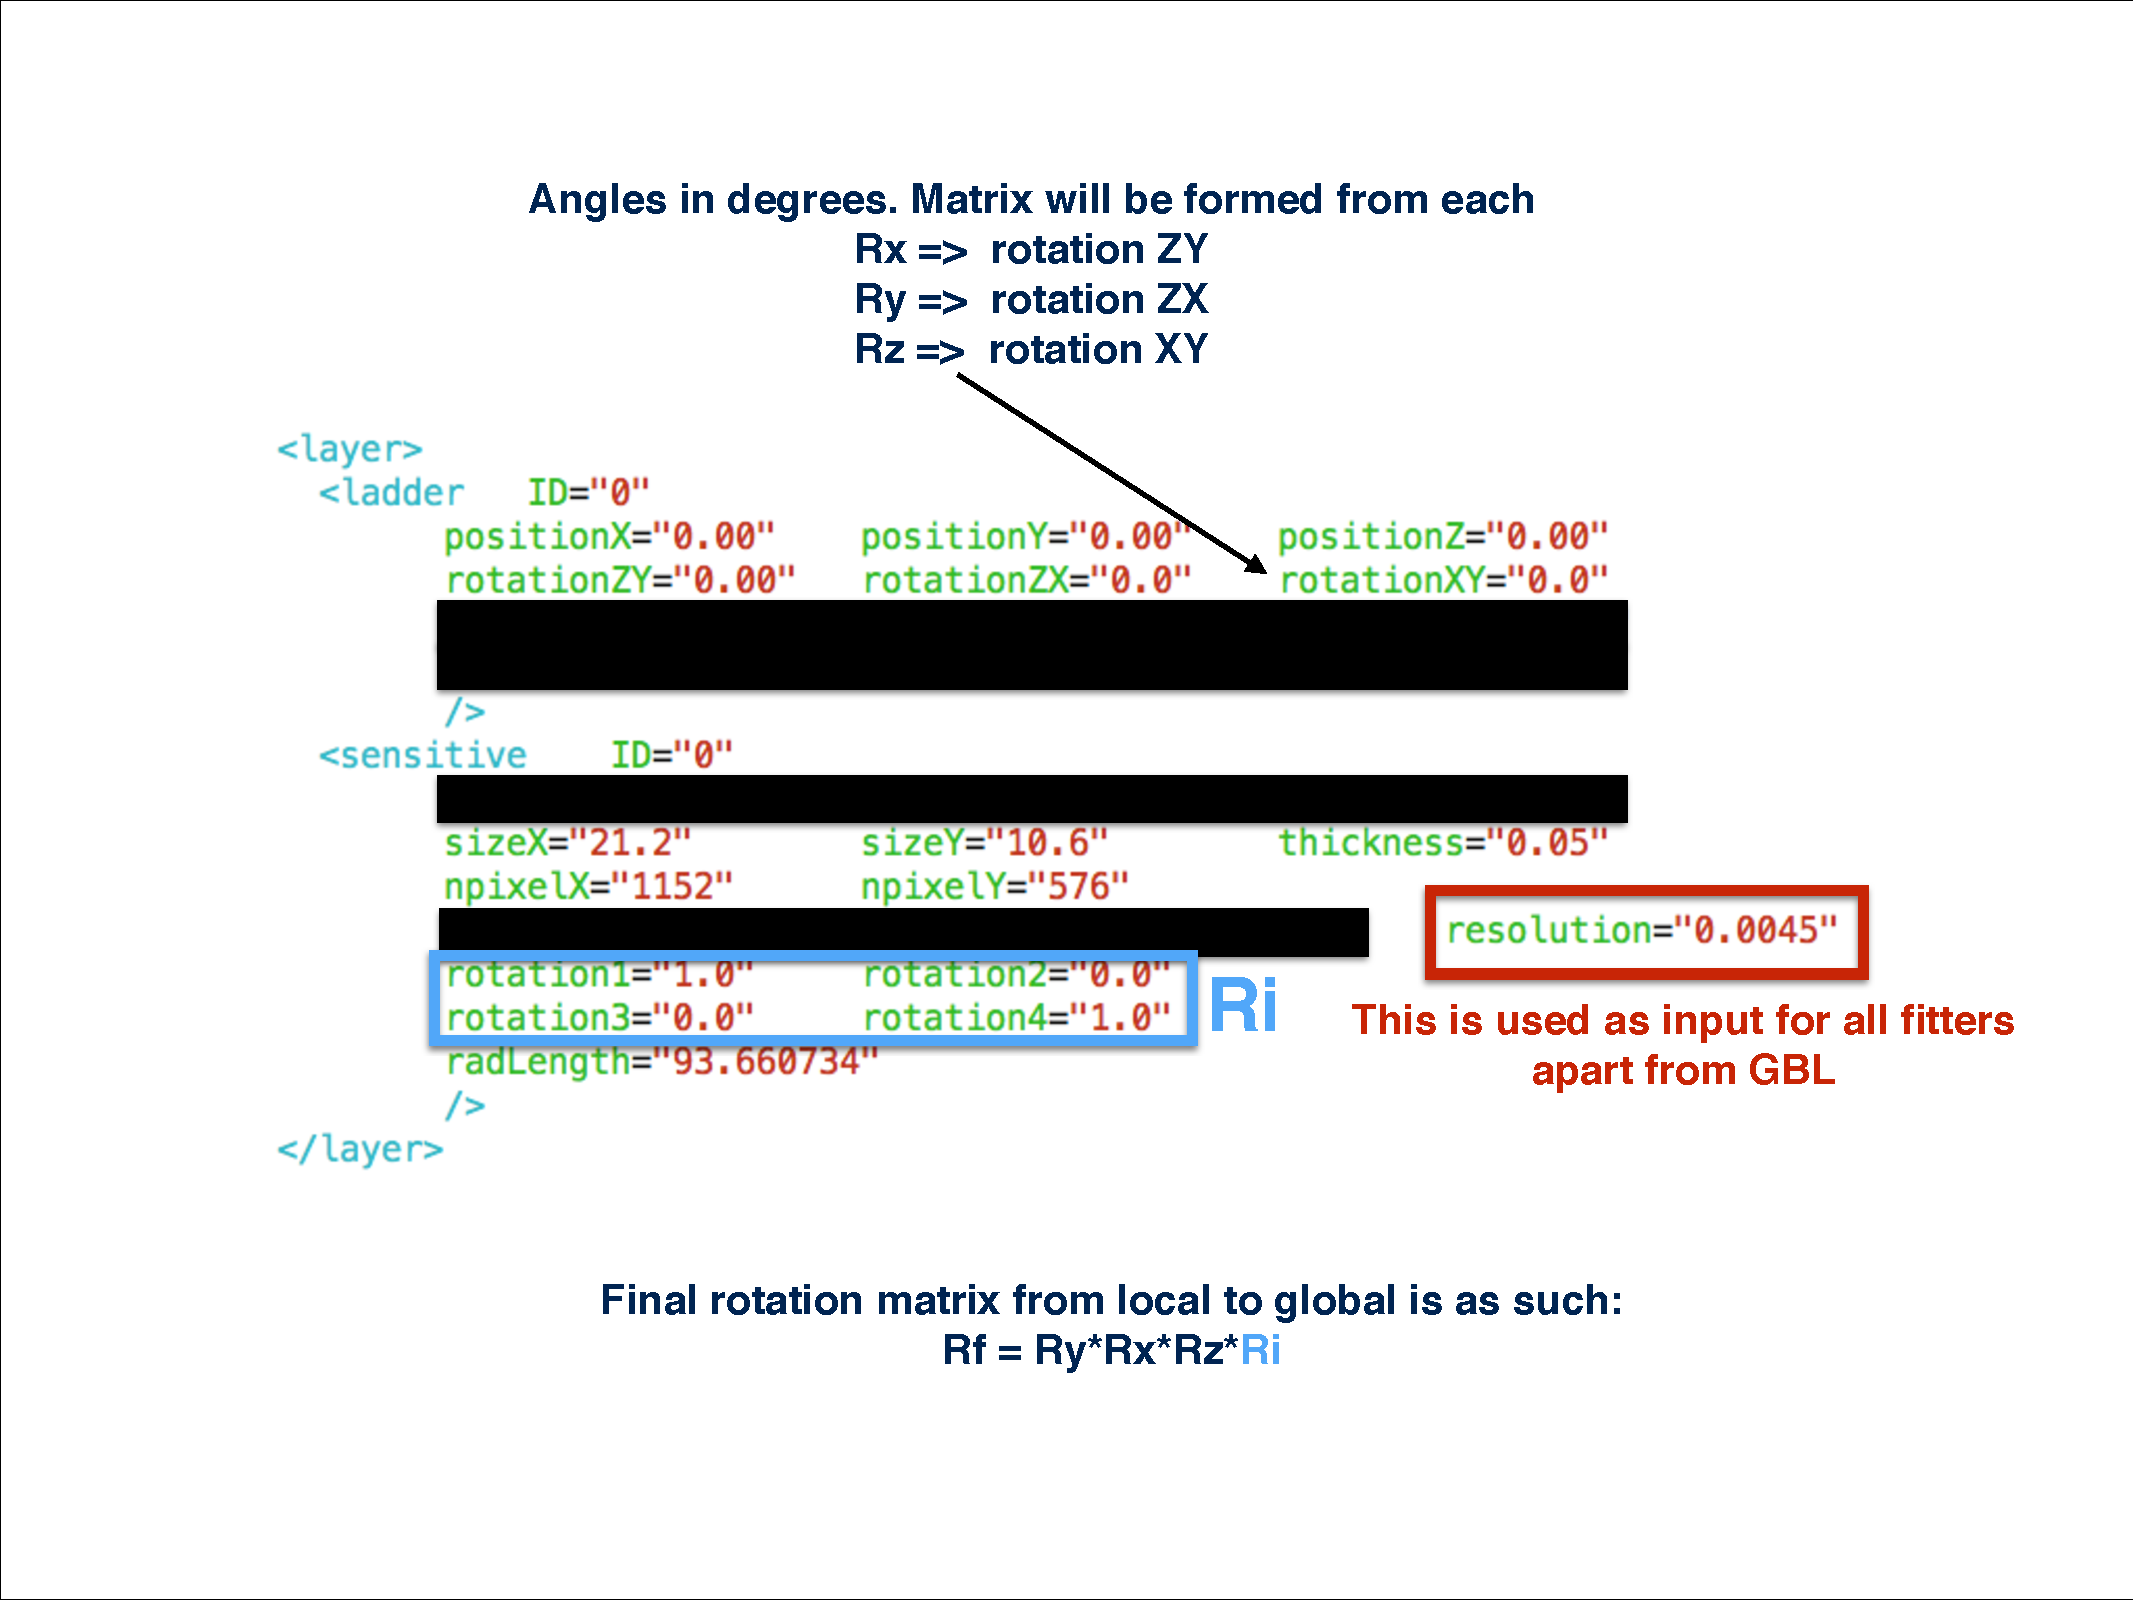
\includegraphics[width=1.0\linewidth]{figures/gear-format.pdf}
\caption{The gear format used with the GBL processor. The black lines are entries not used.}
\label{fig:gear}
\end{figure}

\section{Output format}
Many analyses require the output of the tracking data to be written in a ROOT NTuple format. Two different formats have been created which write the tracks with all clustering information to a ROOT file. Both outputs are used within the SCT example but can be used with any example with an update to the examples' steering files. 

One format was used for the analysis of ATLAS strip data for research concerning the upgrade. This has been used for detailed efficiency measurements. The other format allows the use of TBMon, a large analysis framework were additional selection and analysis can take place.




\clearpage


\chapter{PatternRecognition.}
\label{chp:patRec}
Any pattern recognition can be used with the GBL fitter. This is essential to make the procedure as generic as possible since different forms of pattern recognition are needed for different situations. The only requirement of the GBL fitting processor is a collection of hits which form a track. Parameterisation of the track is done internally and is not required by any new pattern recognition. A basic clustering pattern recognition can be used with the GBL fitter. However the new triplet finder method has been shown to perform better in nearly all scenarios. Therefore this is discussed here and is recommended for most analyses. One negative with this form of pattern recogntion is the requirement of more statistics than a simple clustering technique. This is required due to the low fake rate  of the triplet method. In most cases statistics is not an issue at testbeam. Therefore, if consideration is taken before/during the testbeam on the expected number of reconstructed tracks with a DUT hit then this pattern recognition should be used.

The triplet finder works by associating hits together which have a small distance between each other in the global XY plane. Association of hits must take into account the curvature. This is removed when comparison is done assuming some initial distance traveled through the homogenous magnetic field. A series of cuts are performed and for each cut a selection of possible tracks are excluded. The variables you cut on are put in histograms by the pattern recognition processor. Each cut is an absolute value with some taking the X/Y distance as different cuts. The cut performed are in the following order:

\begin{description} 
\item[DoubletDistCut]  The XY plane distance cut on the outer planes of each arm to create a doublet from two hits. A doublet  is just two hits assumed to come from a track. If the distance between them is below this cut then you create the doublet and this doublet is used in the next cut to look for a triplet. A triplet is just three hits assumed to be a track. Figure \ref{fig:TripForm} shows the doublet on the green planes which will be used to interpolate between to look for a hit on the red plane. 
\begin{figure}[H]
\centering
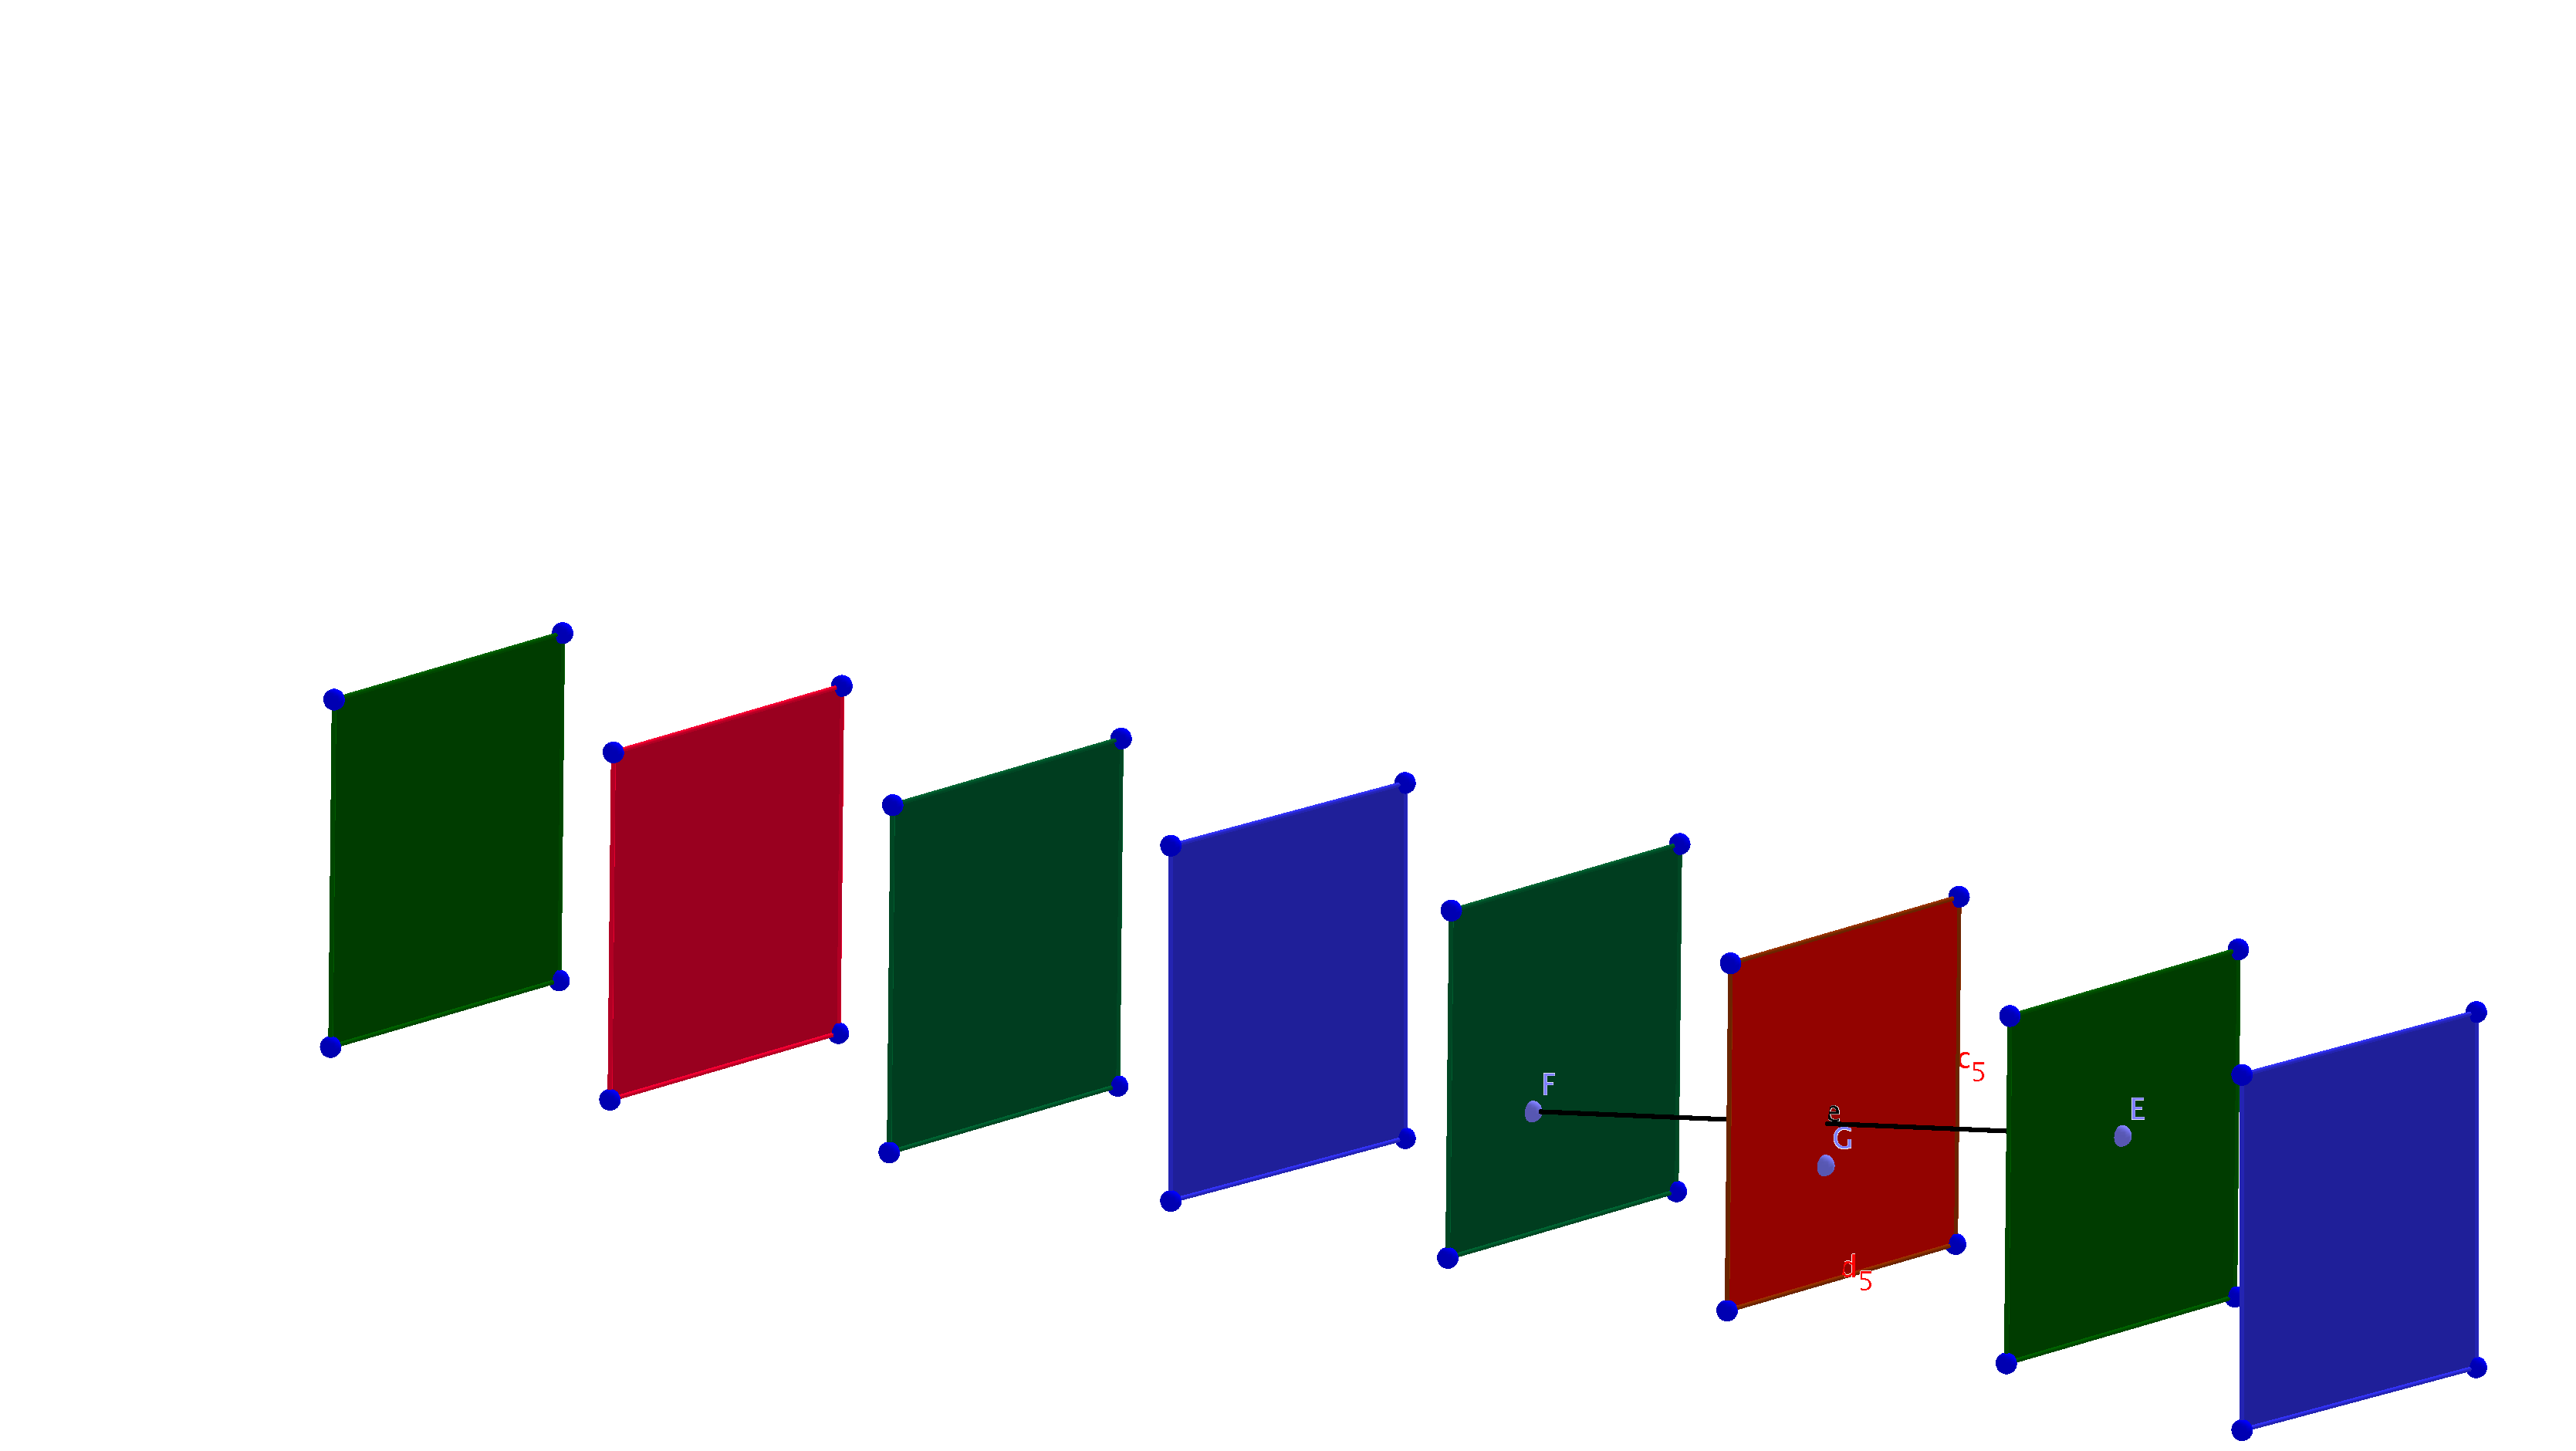
\includegraphics[width=1.0\linewidth]{figures/tripletDoubletFormed.png}
\caption{Doublet which has passed the DoubletDistCut used to look for a triplet. The green planes are used to create the doublets. The red plane with the green planes are used to create the triplets on each arm. The blue planes are DUTs. The blue points are hits.}
\label{fig:TripForm}
\end{figure}

\begin{figure}[H]
\centering
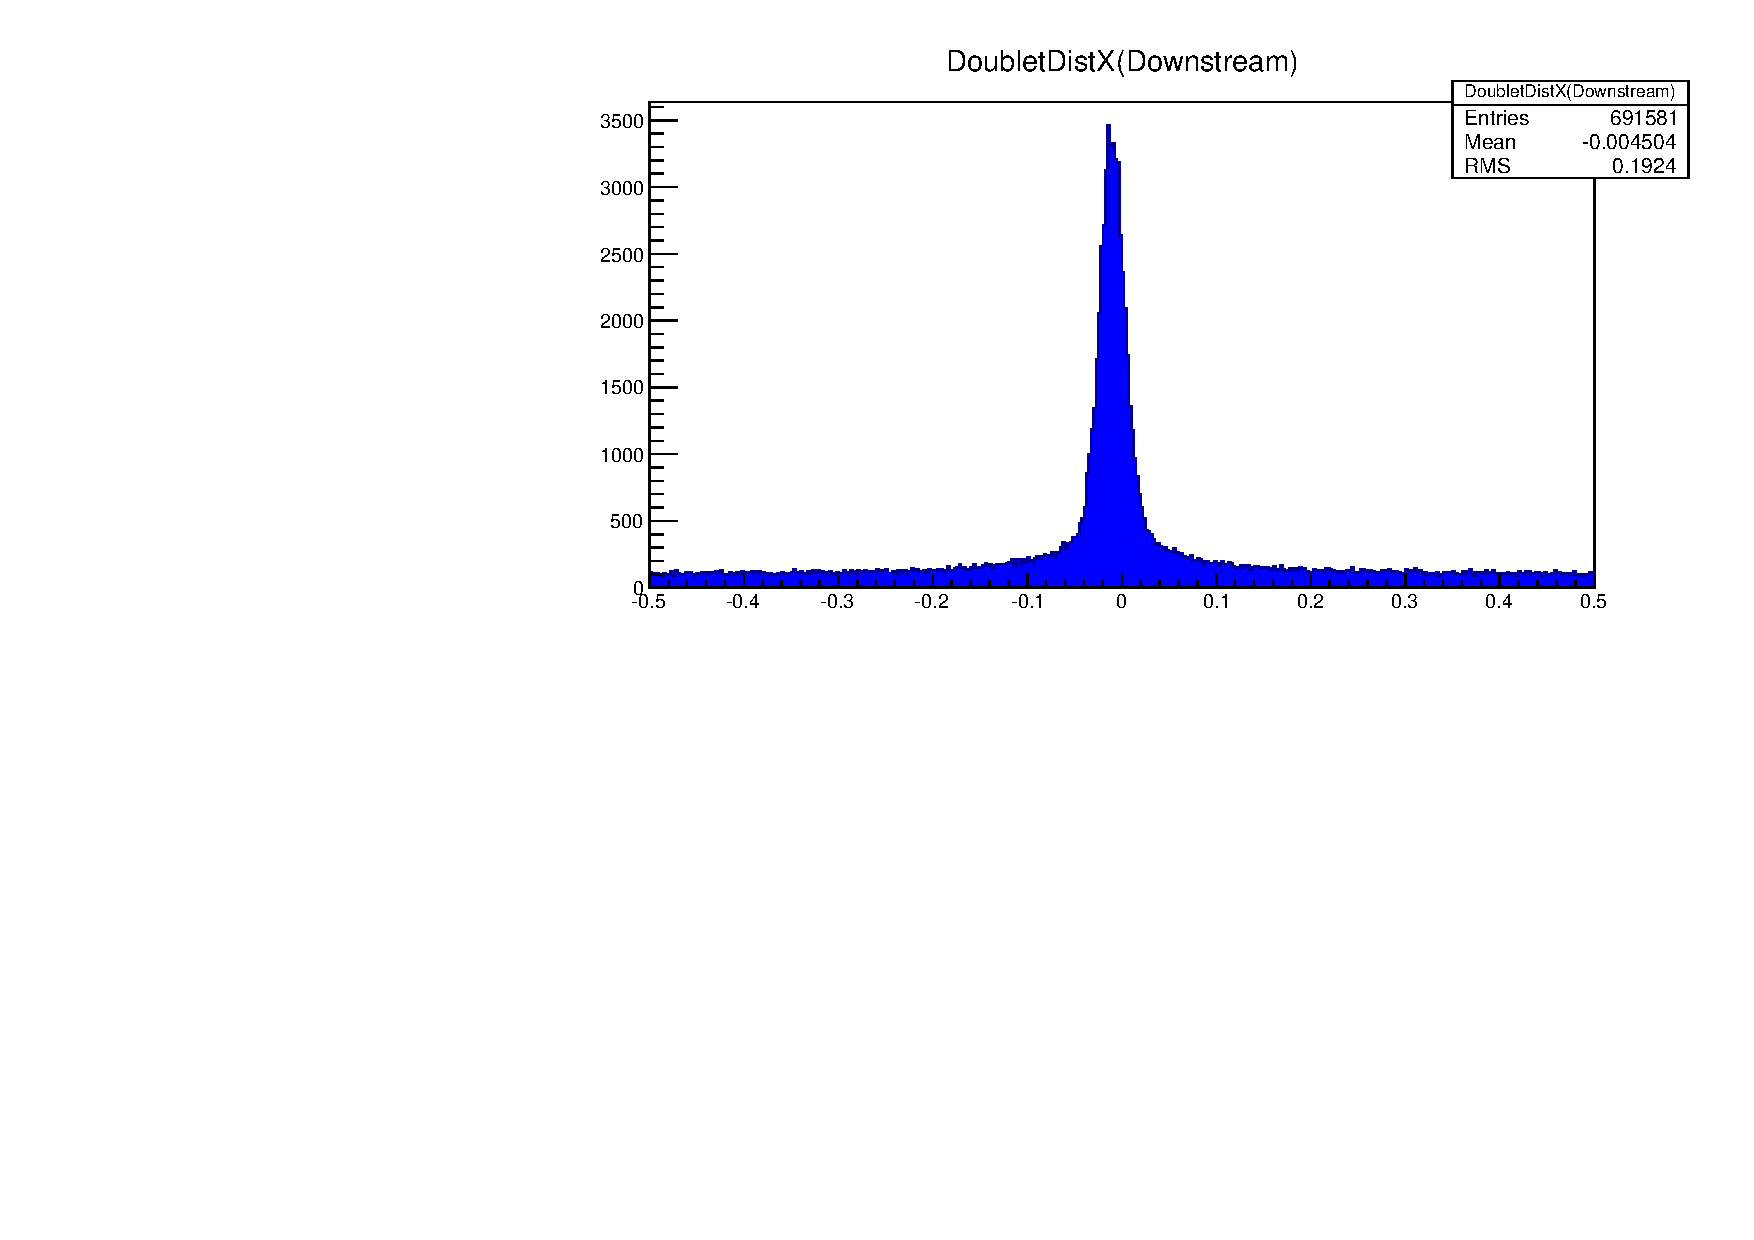
\includegraphics[width=1.0\linewidth]{figures/DoubletDistX-442-preOnly.pdf}
\caption{Doublet distance for down stream arm for DESY testbeam data taken at 4 GeV. This can be used to find the correct cuts for any setup.}
\label{fig:DoubDis}
\end{figure}

\item[DoubletCenDistCut]  The XY plane distance cut on the central planes (Red in figure \ref{fig:TripForm}) and prediction from doublet to create triplet . 

\begin{figure}[H]
\centering
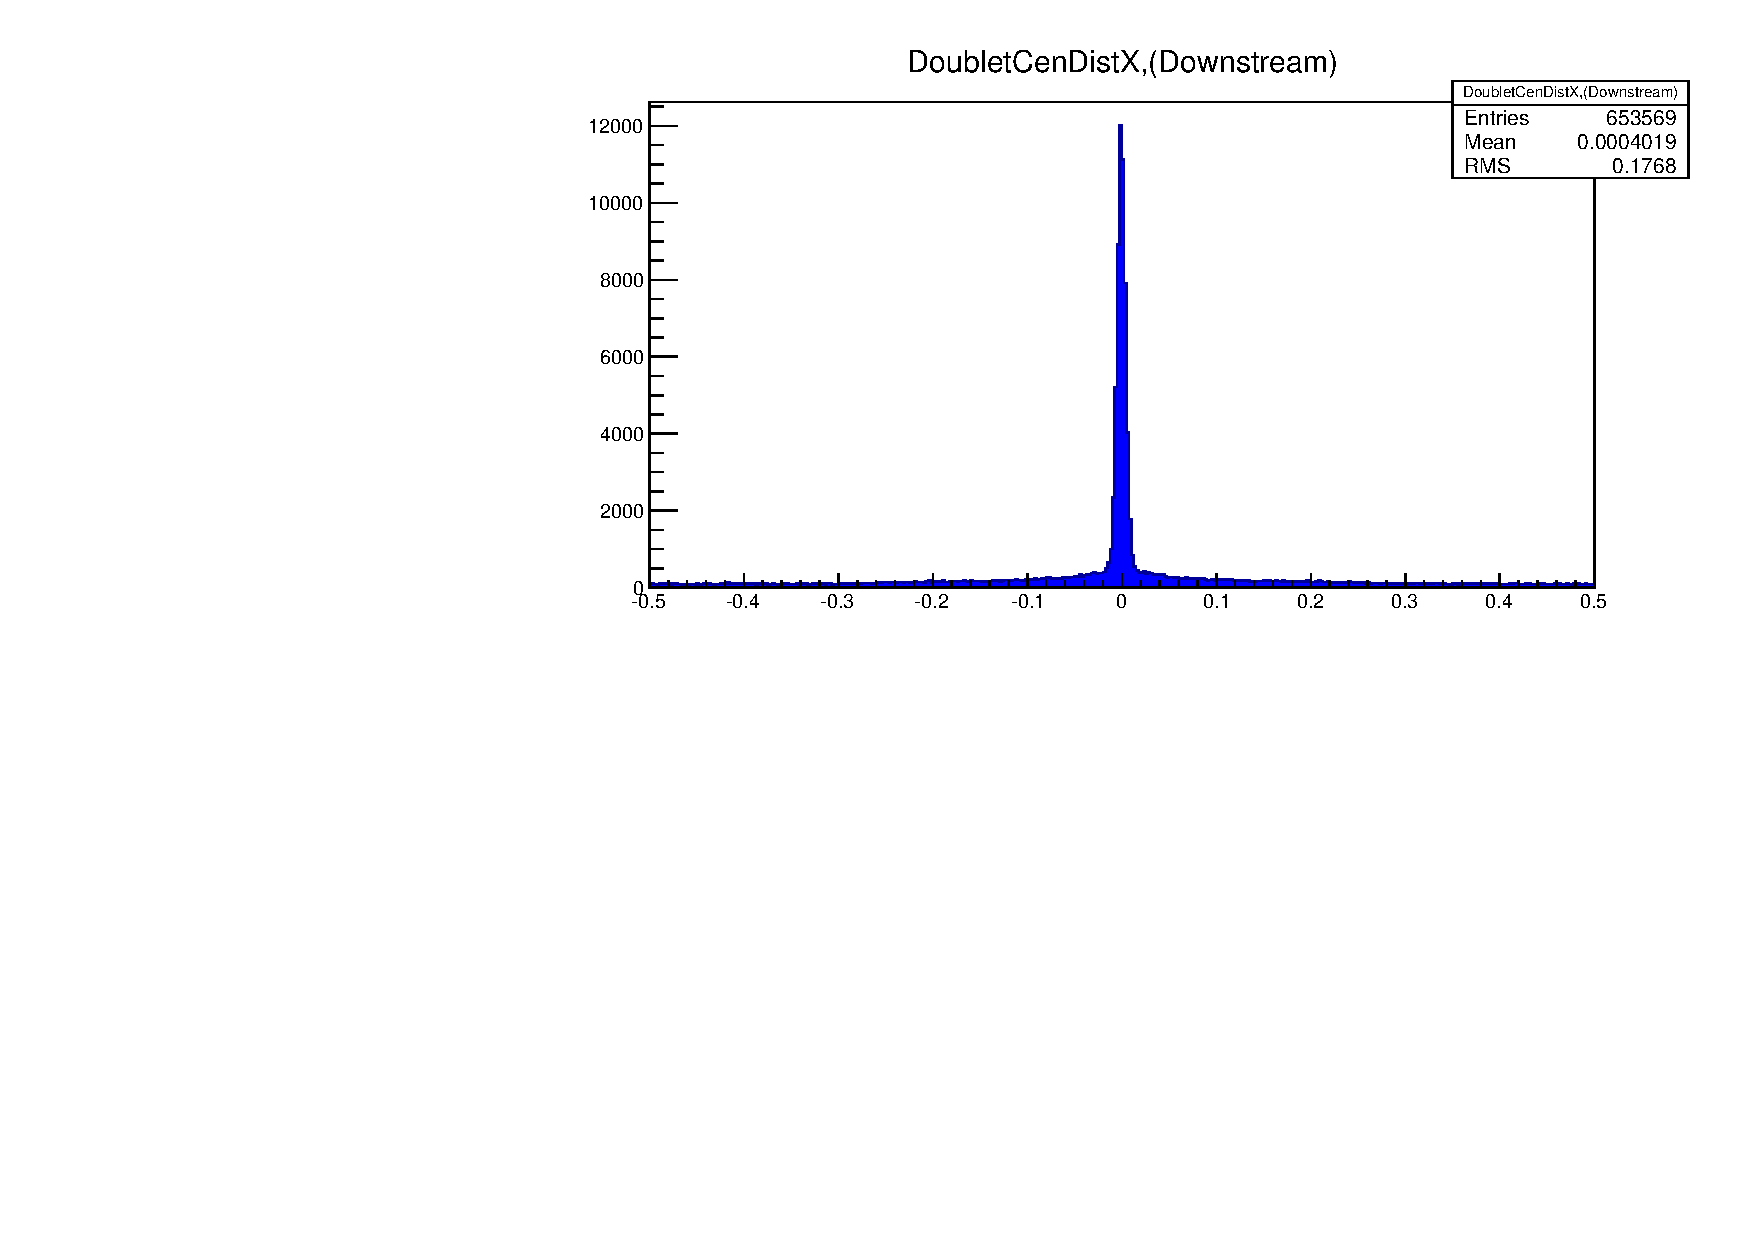
\includegraphics[width=1.0\linewidth]{figures/DoubletCenDist-442.pdf}
\caption{Doublet distance to central hit for down stream arm.}
\label{fig:DoubCen}
\end{figure}

\item[TripletConnectDistCut]  The triplets formed which pass the cuts are associated together using each triplet extrapolated to the centre of both triplets. With each triplet's position defined as the centre of of the doublet. This can be seen in figure \ref{fig:TripCon} were the triplets are extrapolated to a central point near the central DUT (DUTs in blue).

\begin{figure}[H]
\centering
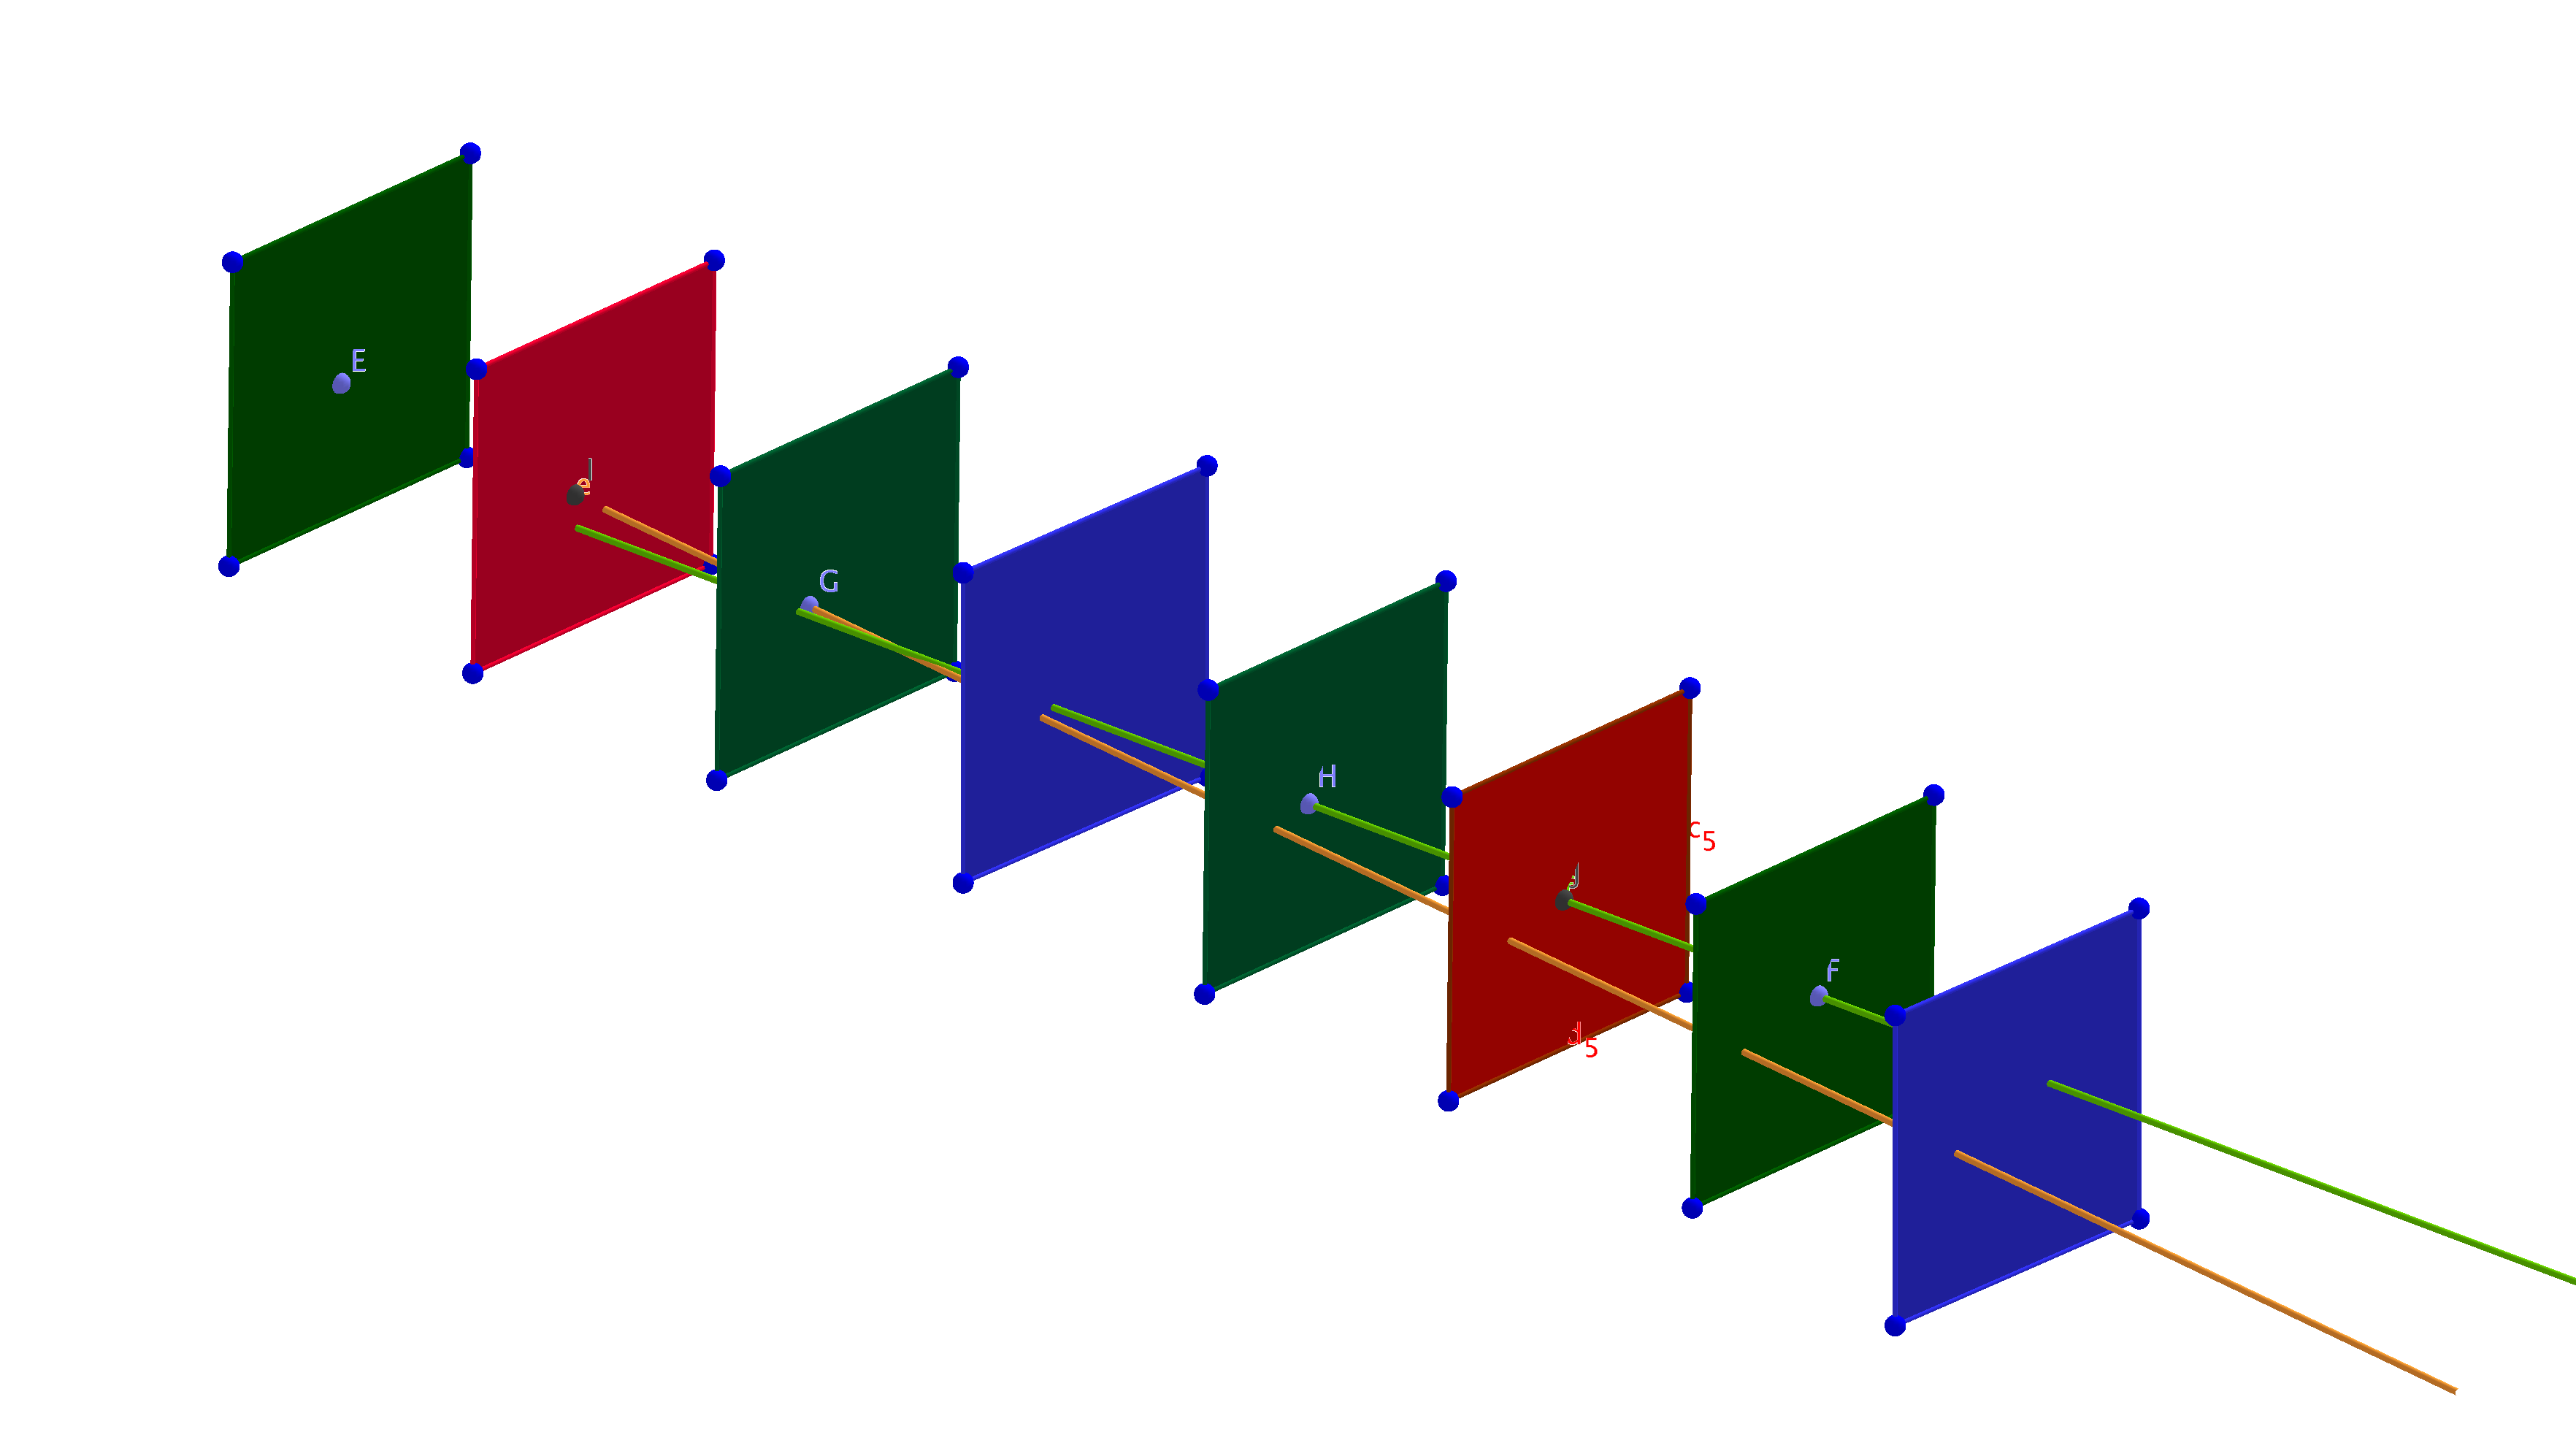
\includegraphics[width=1.0\linewidth]{figures/tripletsconnect.png}
\caption{A central point is used between both arms to compare both triplets' prediction. Each triplet is formed from the green and red planes of each arm. }
\label{fig:TripCon}
\end{figure}

\begin{figure}[H]
\centering
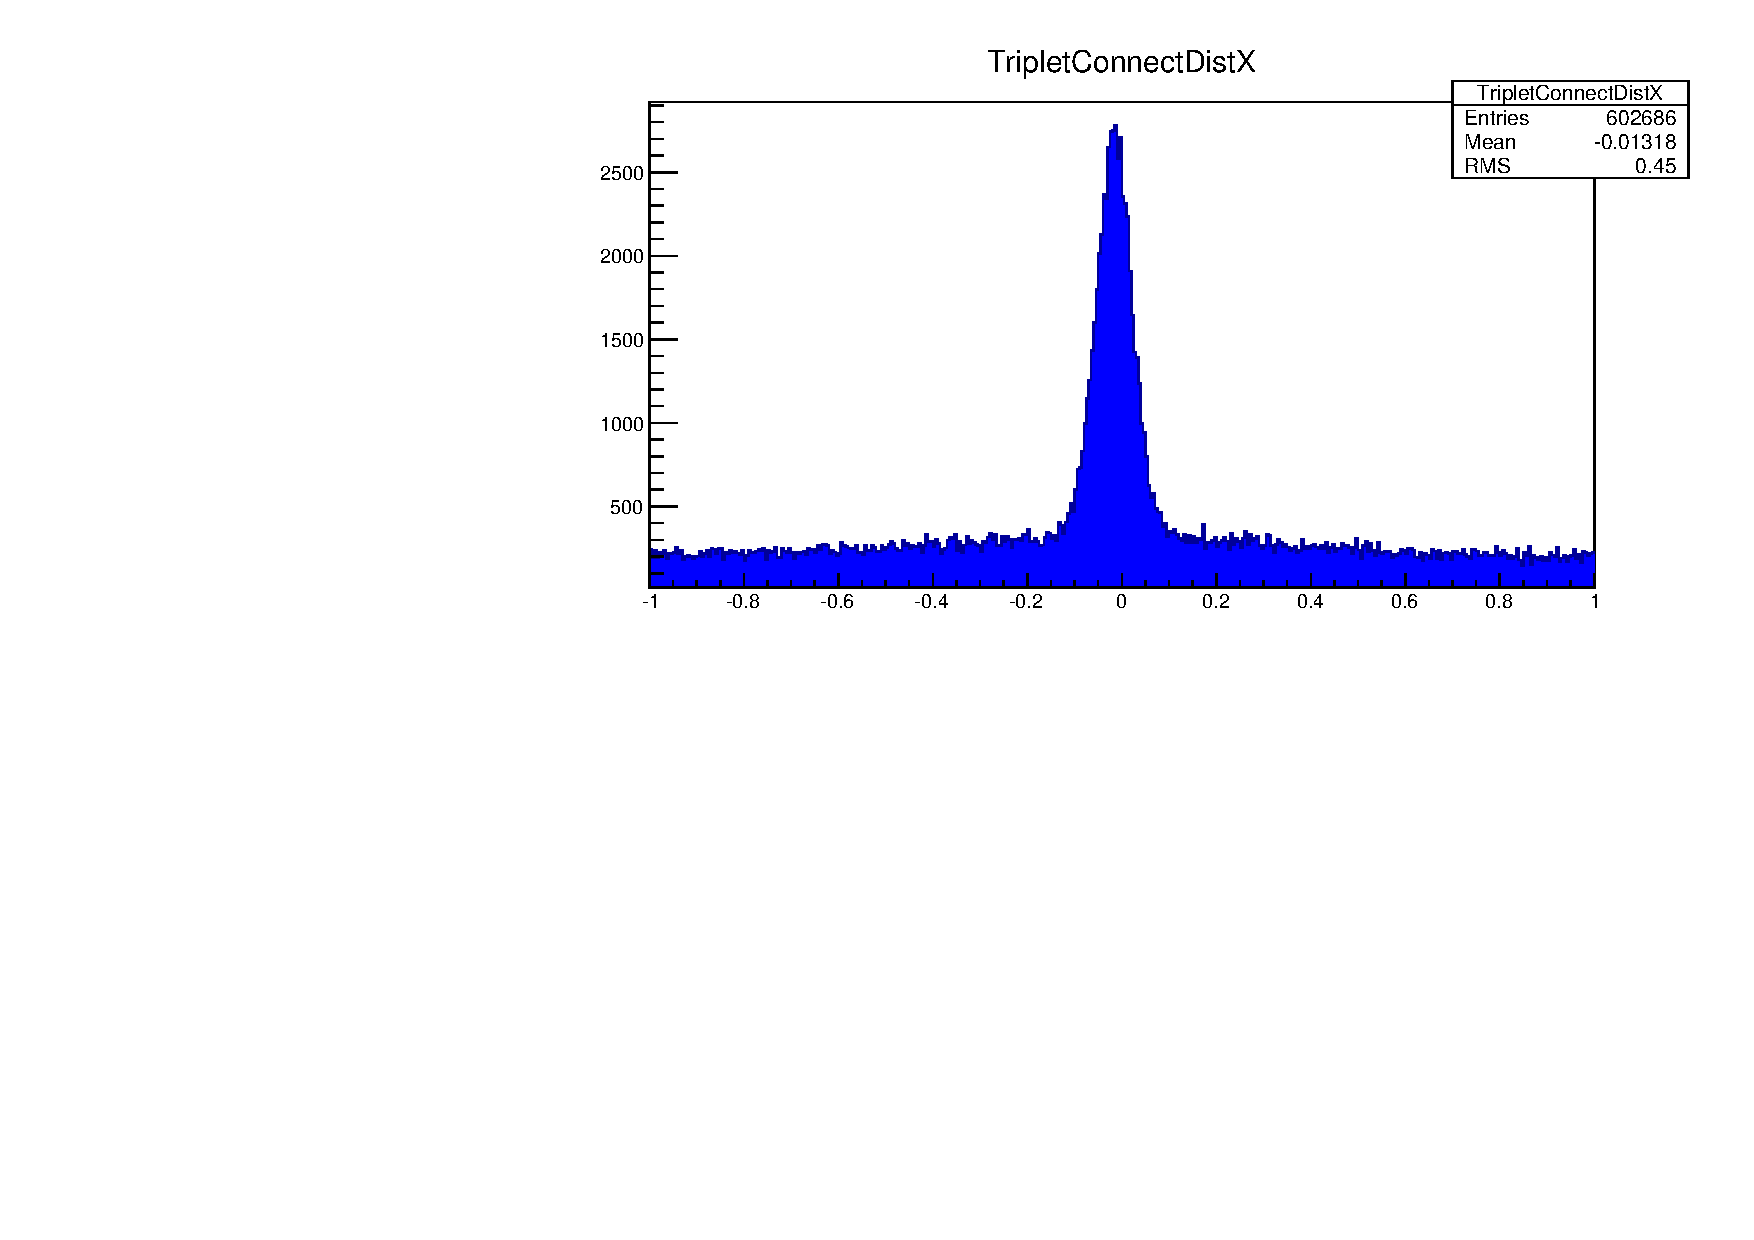
\includegraphics[width=1.0\linewidth]{figures/TripletConnectDistX-442.pdf}
\caption{The distance between the two triplet predictions at some central point.}
\label{fig:TripCen}
\end{figure}

\item[TripletSlopeCut] Figure \ref{fig:TripCon} shows that the prediction of both triplets can be accurate but the slope wrong. Therefore a slope cut between the two triplets must be applied. Testbeam setups in most cases only have a small beam divergence so this does not have to be precise.
\newline
\newline 
beam divergence = approx 1/0.5 mRad (DESY/SLAC)
\newline
\newline
The final track produced before the addition of DUT hits must come from a unique matching of triplets. If a triplet on one arm is matched with two triplets on the other then the triplet with two matches is removed.

\item[DUTWindow] After the triplets are associated together then the DUT hits are attached to this track if the hit is within some minimum distance. 
\begin{figure}[H]
\centering
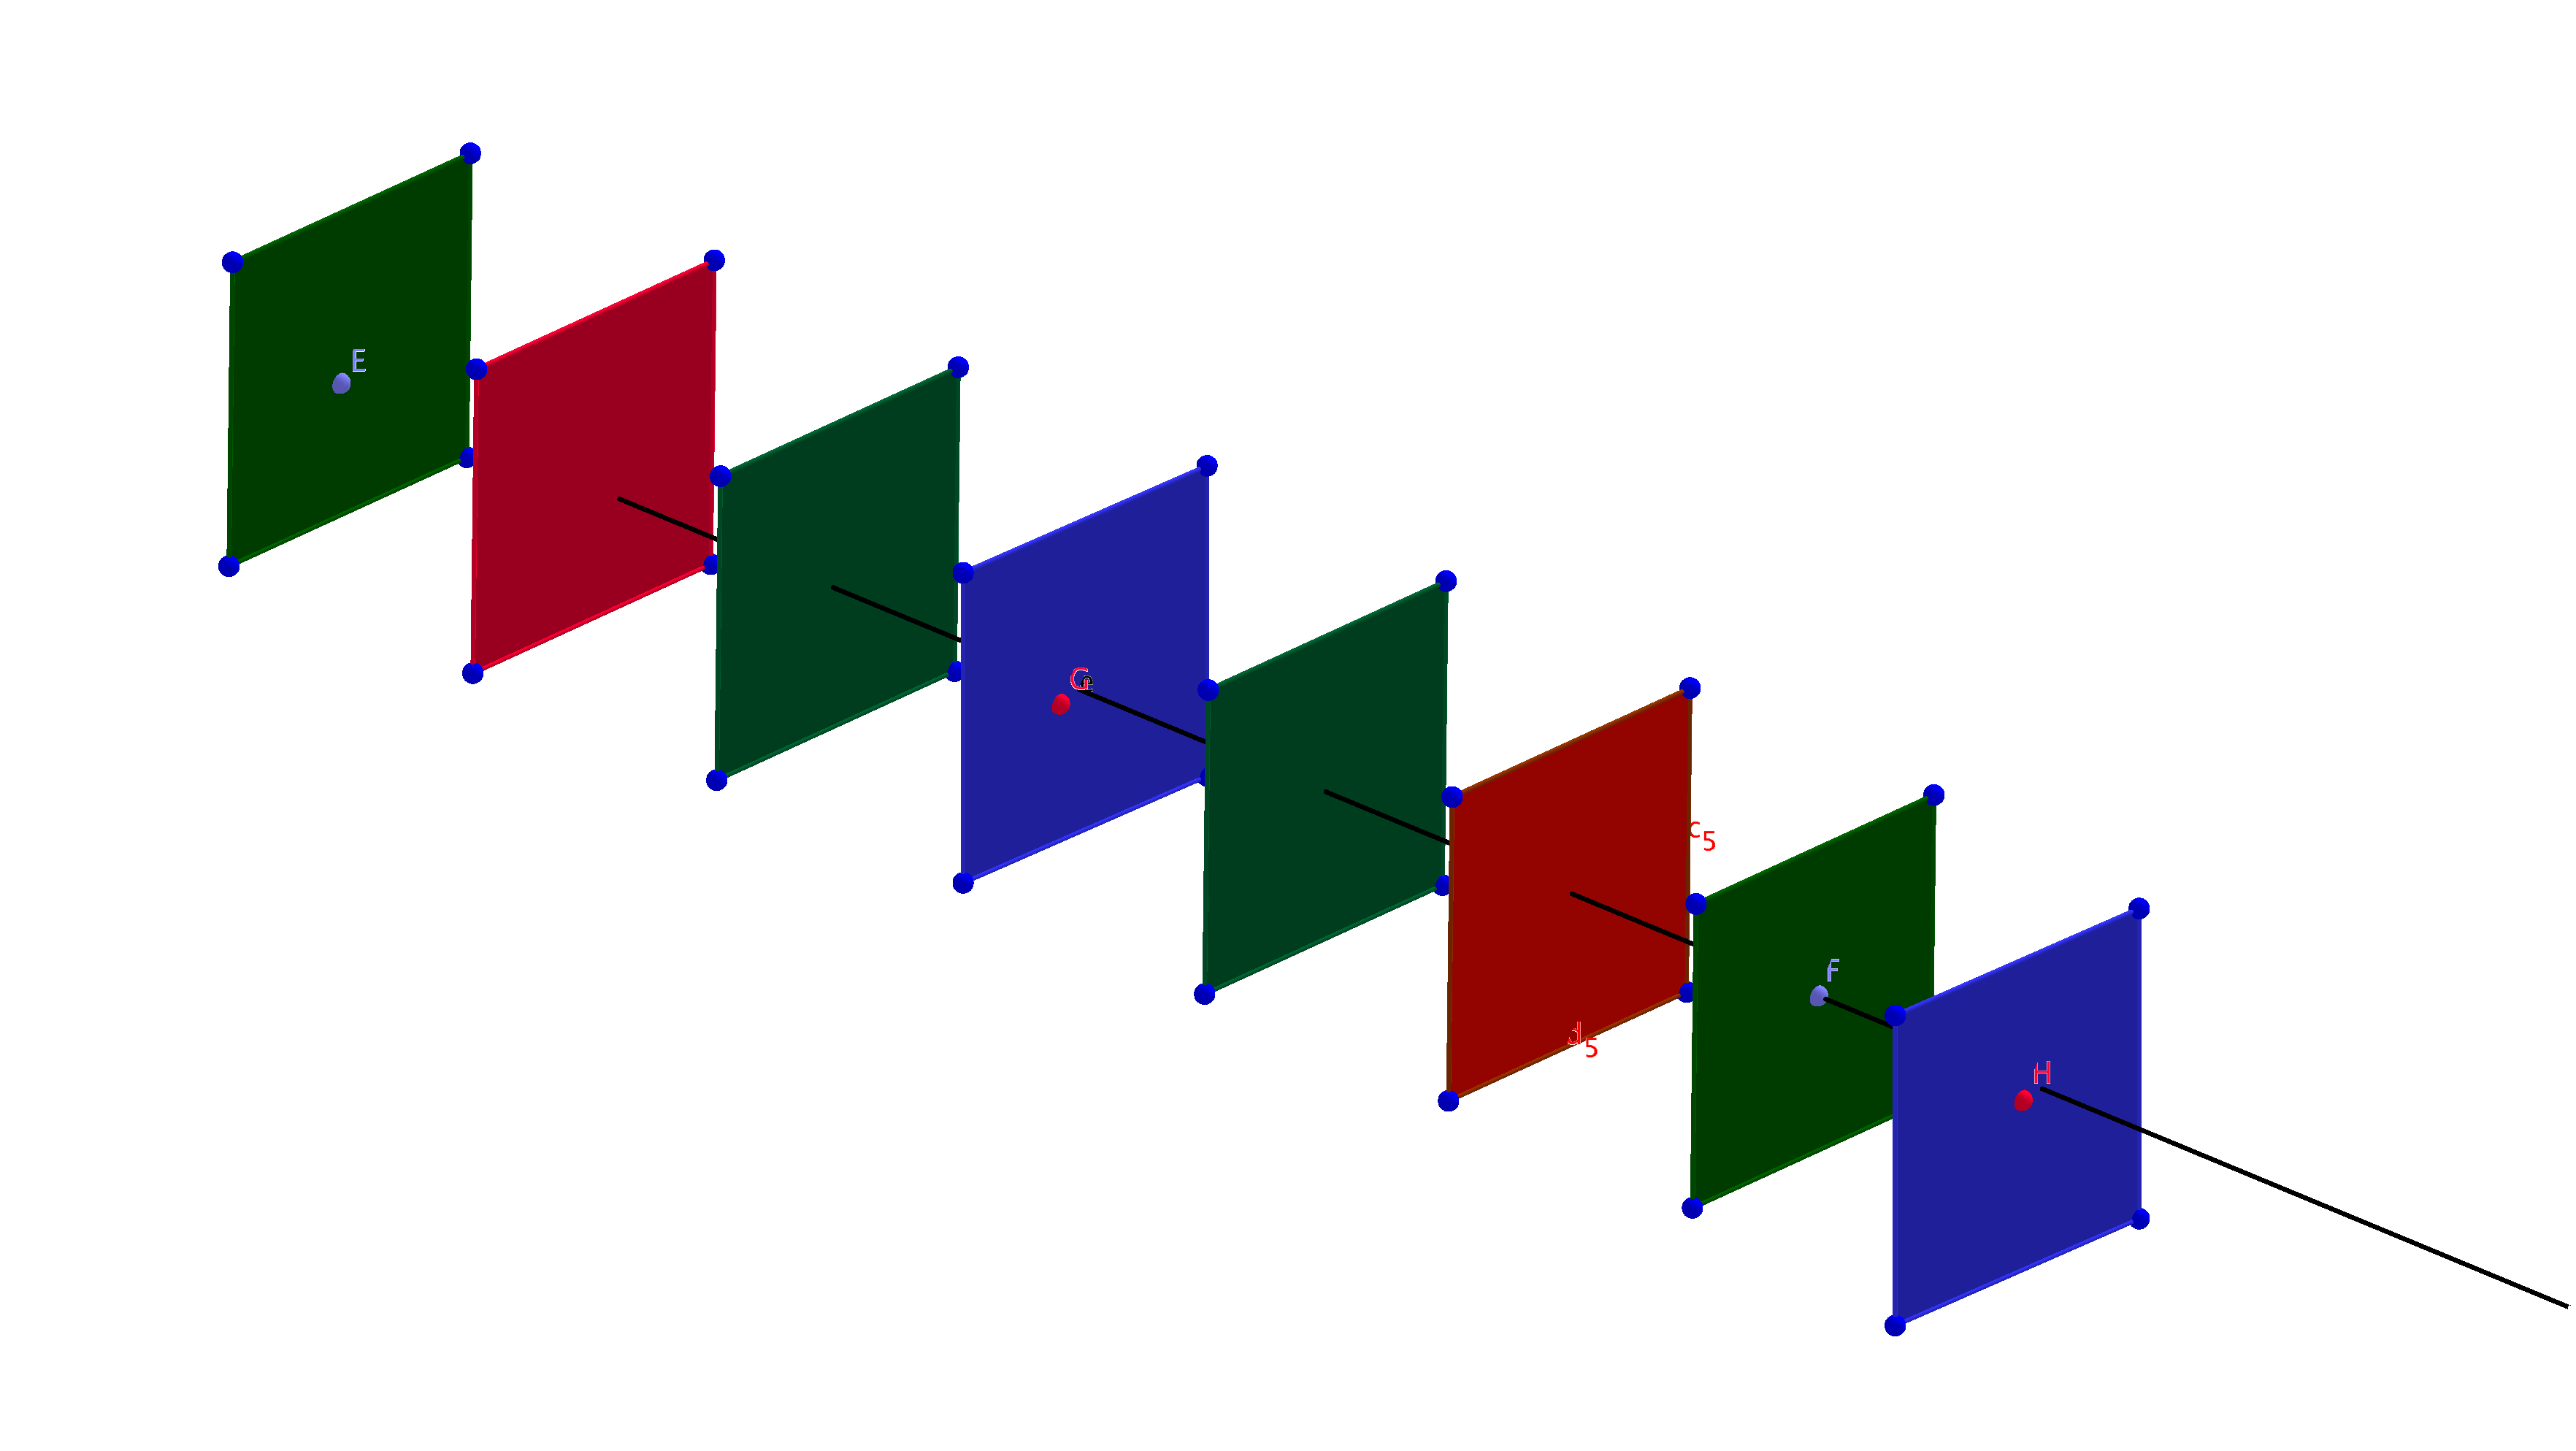
\includegraphics[width=1.0\linewidth]{figures/DUThitsPat.png}
\caption{The red dots on the blue DUT planes are hits. If the track produced by the mimosas is close to these hits then attach the hits to the track.}
\label{fig:DoubDis}
\end{figure}


\end{description}

Unique matching between a single DUT hit and a track must be found. If a track or hit is associated twice then the hit/track is removed from fitting with a DUT hit on that plane. All tracks produced by the mimosas are returned regardless of there being a DUT hit attached.

The hits collected which have been identified are assumed to come from a single track. How this track is described or parameterised depends on how accurate you want to be. Note parameterising is just the same as fitting, however to use the GBL algorithm you need an initial "guess". This initial guess must include positions, incidences, kink angles and curvature. The kink angles are fitted as parameters within GBL in contrast to many fitters which includes this as additional non diagonal variance in the propagated error matrix. In all examples this is not required and a single iteration of the GBL fitter with the basic internal parameterisation will suffice.





\clearpage
\chapter{Fitting and Alignment.}
\label{chp:gbl}
The information needed to use the GBL algorithm is the same of any track fitting method. Therefore the information provided here can be used with any fitting procedure. The only difference is the underlying "engine" which is used, in this case GBL. The construction of a track which can be used for alignment or analysis is done in five steps. The order does not pattern except the linking of trajectory points must be done before anything else. Each step will be covered in turn. 
\section{The five fold way}
\subsection{Linking trajectory points}
The initial requirement for track fitting is a coordinate system which links the local and global frames. The local frame is defined by the readout layout of the sensor, a Cartesian grid over the surface of the sensor and is unique for each DUT. The global frame is a Cartesian grid which extends over the full detector system. This is the same for all DUTs and alignment is needed to link both these frame for each DUT. Each plane is linked to the same global frame using the transformation:
\begin{equation}
 \overrightarrow{G} =   \hat{R}\overrightarrow{L} +  \overrightarrow{O}
\end{equation}

were the rotation matrix is defined

\begin{equation}
 \hat{R} = \hat{R_Y}\hat{R_X}\hat{R_Z}\hat{R_I}
\end{equation}

with $R_{X/Y/Z}$ as rotations in that particular axis. $R_I$ is the initial rotation matrix which can be set in gear to whatever value you see fit. The definition of these matrices come from TGeo manager and are documented online. Note the offsets are defined in the global frame since they are applied after all rotations. 

The order of applying transformations matters and must be considered. This is important for alignment and is discussed in section \ref{gloPar}. All large rotations round the X/Y axis must be applied as transforms to the initial matrix. If you apply this transform to $R_Y$/$R_X$ then the alignment matrix will not correspond to the correct frame for the rotation corrections. This can be ignored for rotations about 30 degrees. However if mapping between the local and global frame swaps axis then this is too large to adjust for and should be applied to the matrix $R_I$. The small changes to the rotations from alignment is applied to $\hat{R_Z}$,  $\hat{R_Y}$ and $\hat{R_X}$.


The full trajectory of a track does not need to be modeled for an accurate fit. Locations of high scattering and with measurements must be added. These points must be linked together using some Jacobian. A Jacobian in this case is just a link between how changes in position/incidence on one plane affects another. Curvature is an additional fitting term which is common to the track and does not vary with position. The Jacobian used to link the points together is 


\begin{center}
$
 \left( \begin{array}{cccccc}
1                            & 0       & 0        & 0 & 0  \\
\frac{F(0)ds}{dz} & 1        & 0        & 0 & 0  \\
\frac{F(1)ds}{dz} & 0        & 1        & 0 & 0  \\
0.5F(0)ds^2        & dz*ds & 0        & 1 & 0      \\  
0.5F(1)ds^2        & 0        & dz*ds & 0 &  1       \\  
  \label{eq:PC}
\end{array}
 \right)
$
\captionof{table}{The Jacobian used to link discrete points to form a continuous track. dz is the normalized direction of the track along z. ds is the arc length to the next point. F() is a vector which is the curvature of the track which depends on the energy and magnetic field the particle is immersed in.}
\end{center}

\begin{figure}[H]
\centering
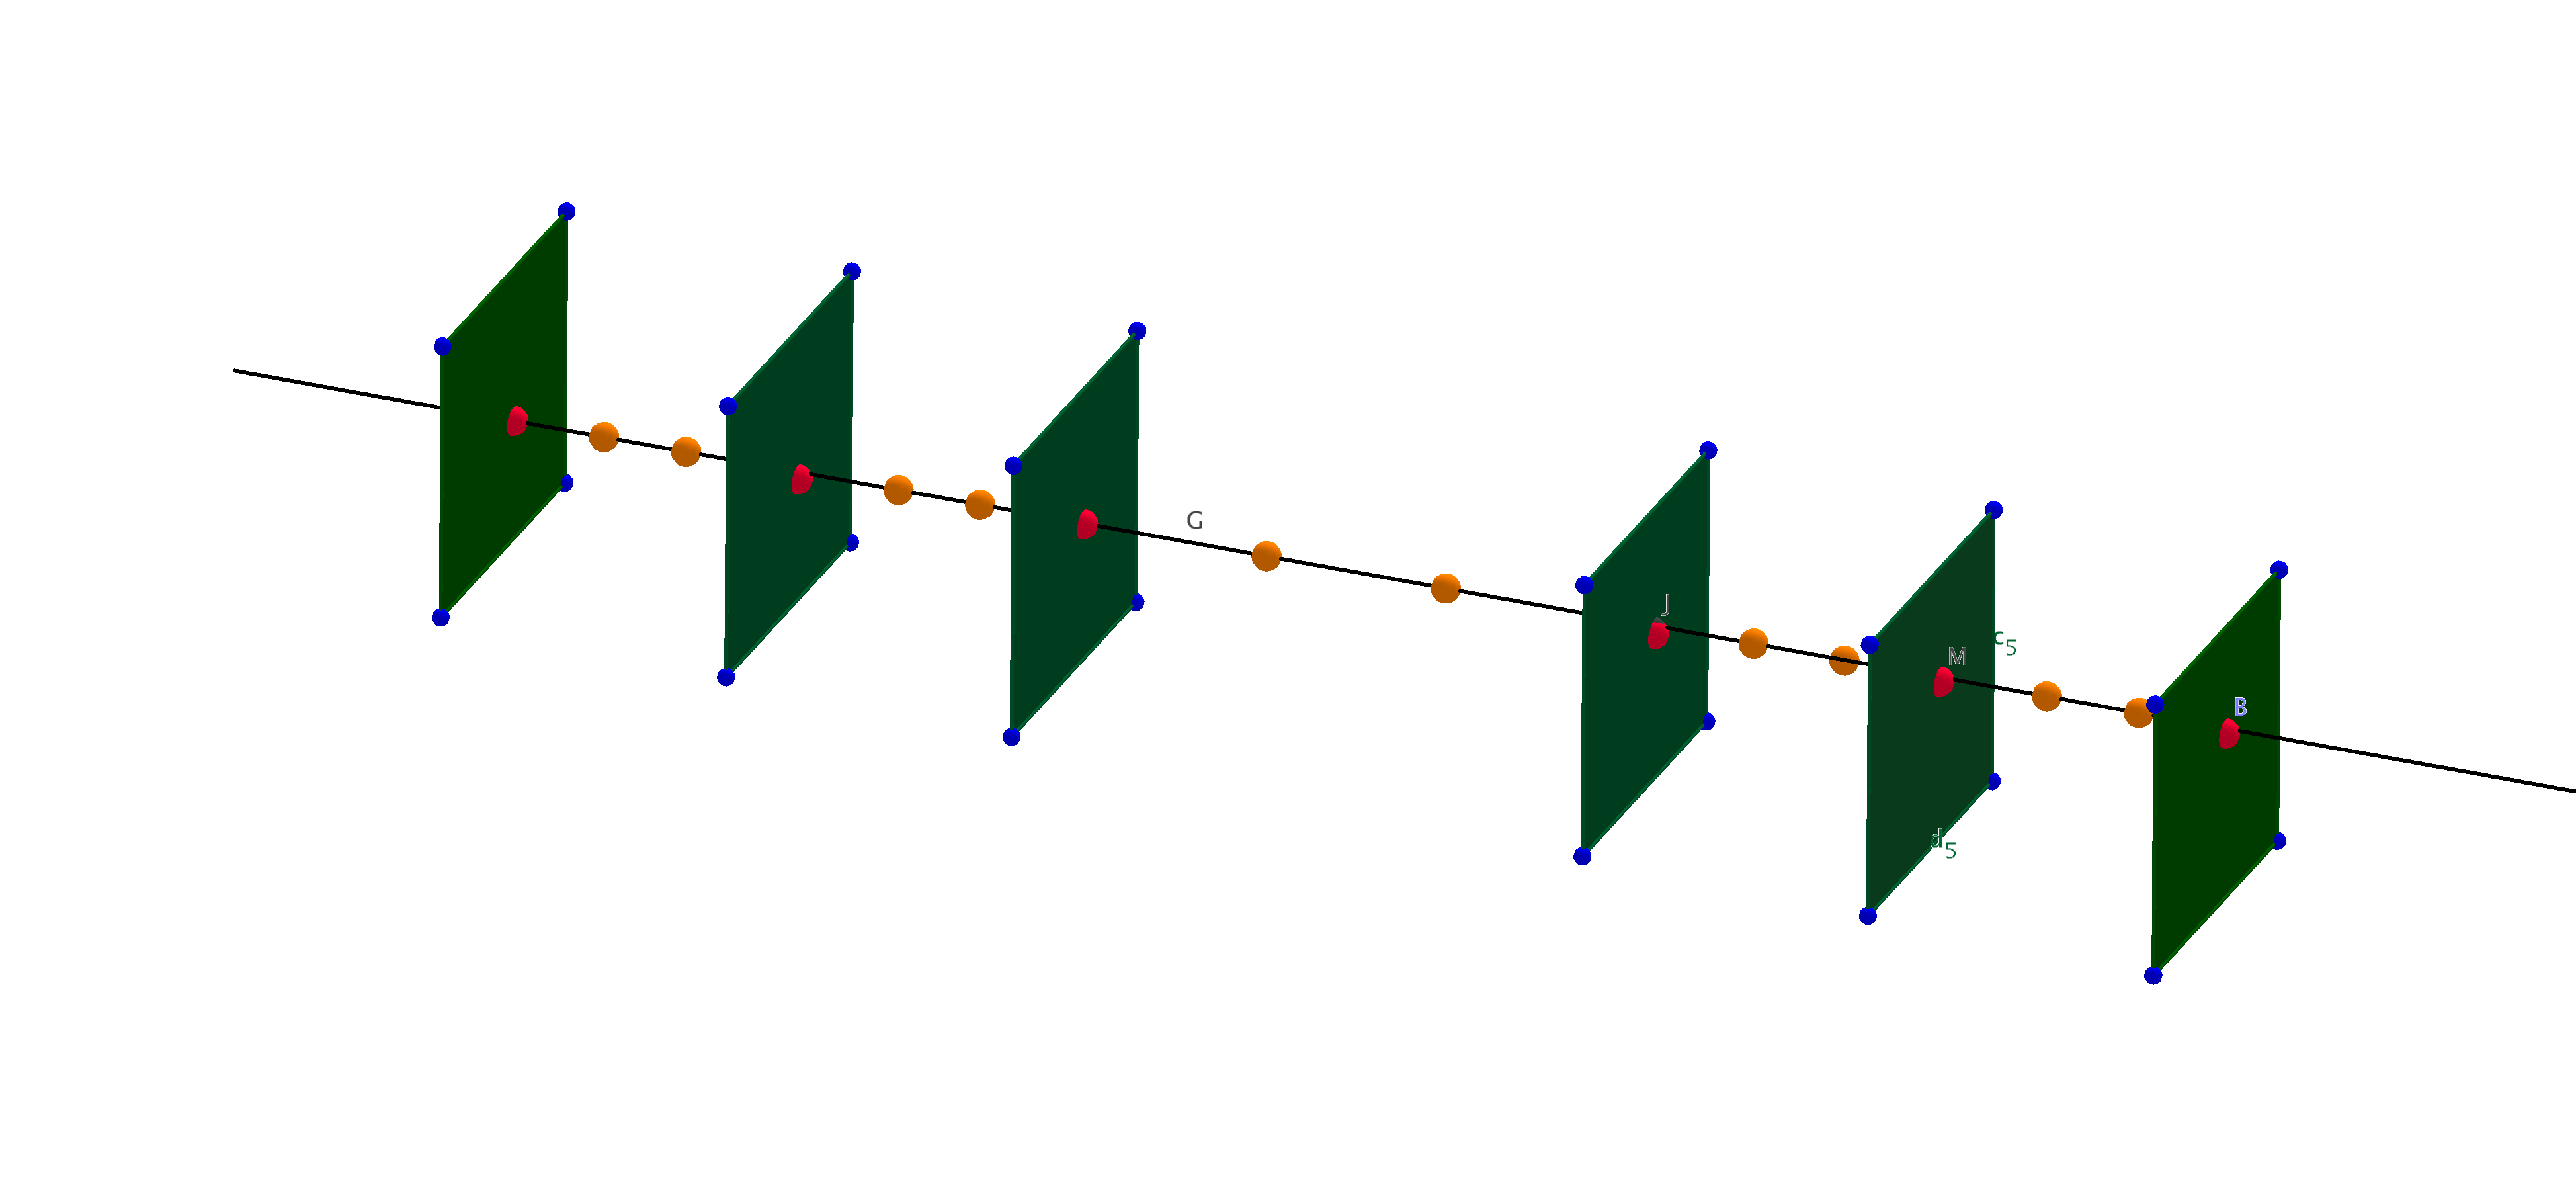
\includegraphics[width=1.0\linewidth]{figures/meas-scat-jac-link.png}
\caption{The red points have measurement and scattering information. The yellow points only scattering information. Measurements are the hit positions in the local frame. Scattering information is the kink angles measured in the local frame. Both have associated errors which must be determined. The Jacobian links all these point together so a change in one will affect a change in another.}
\label{fig:LinkJac}
\end{figure}


What points and where depend on the location of the measurement planes and the scattering from all the material. In the EUTelescope case a single point is used for each measurement and the material in front of this until the next measurement is associated with two points. Two points are need to describe a thick scatterer which is discussed in section \ref{sec:scat}. The linking of the full trajectory is done in the global frame.

\subsection{Add measurement information to points}

The measurements on the planes must be added to the trajectory created. The measurements are the residuals (Measured-Predicted) and the associated errors. The trajectory is always in the global frame and each measurement plane will not always be in this frame. Therefore propagation between the global and local frame is needed to link this information.
The propagation matrix used is

\[ 
\left( \begin{array}{ccc}
1  & 0   & -\frac{dx}{dz}   \\
0   & 1  & -\frac{dy}{dz}  
  \label{eq:prop}
\end{array}
 \right)
  \left( \begin{array}{cc}
 \overrightarrow{Rx}  &  \overrightarrow{Ry}  
\end{array}
 \right)
 \] 
 
 with slope defined in the local frame.  $\overrightarrow{Rx}$ and  $\overrightarrow{Ry}$ are the local X/Y axis defined in the global frame. The first matrix will transform the position from global to local frame. You only need to apply the partial rotation matrix since there should be no z displacement in this frame. The second part will determine the intersection on the XY plane in the local frame from a track propagated to the new local position.
 
 \begin{figure}[H]
\centering
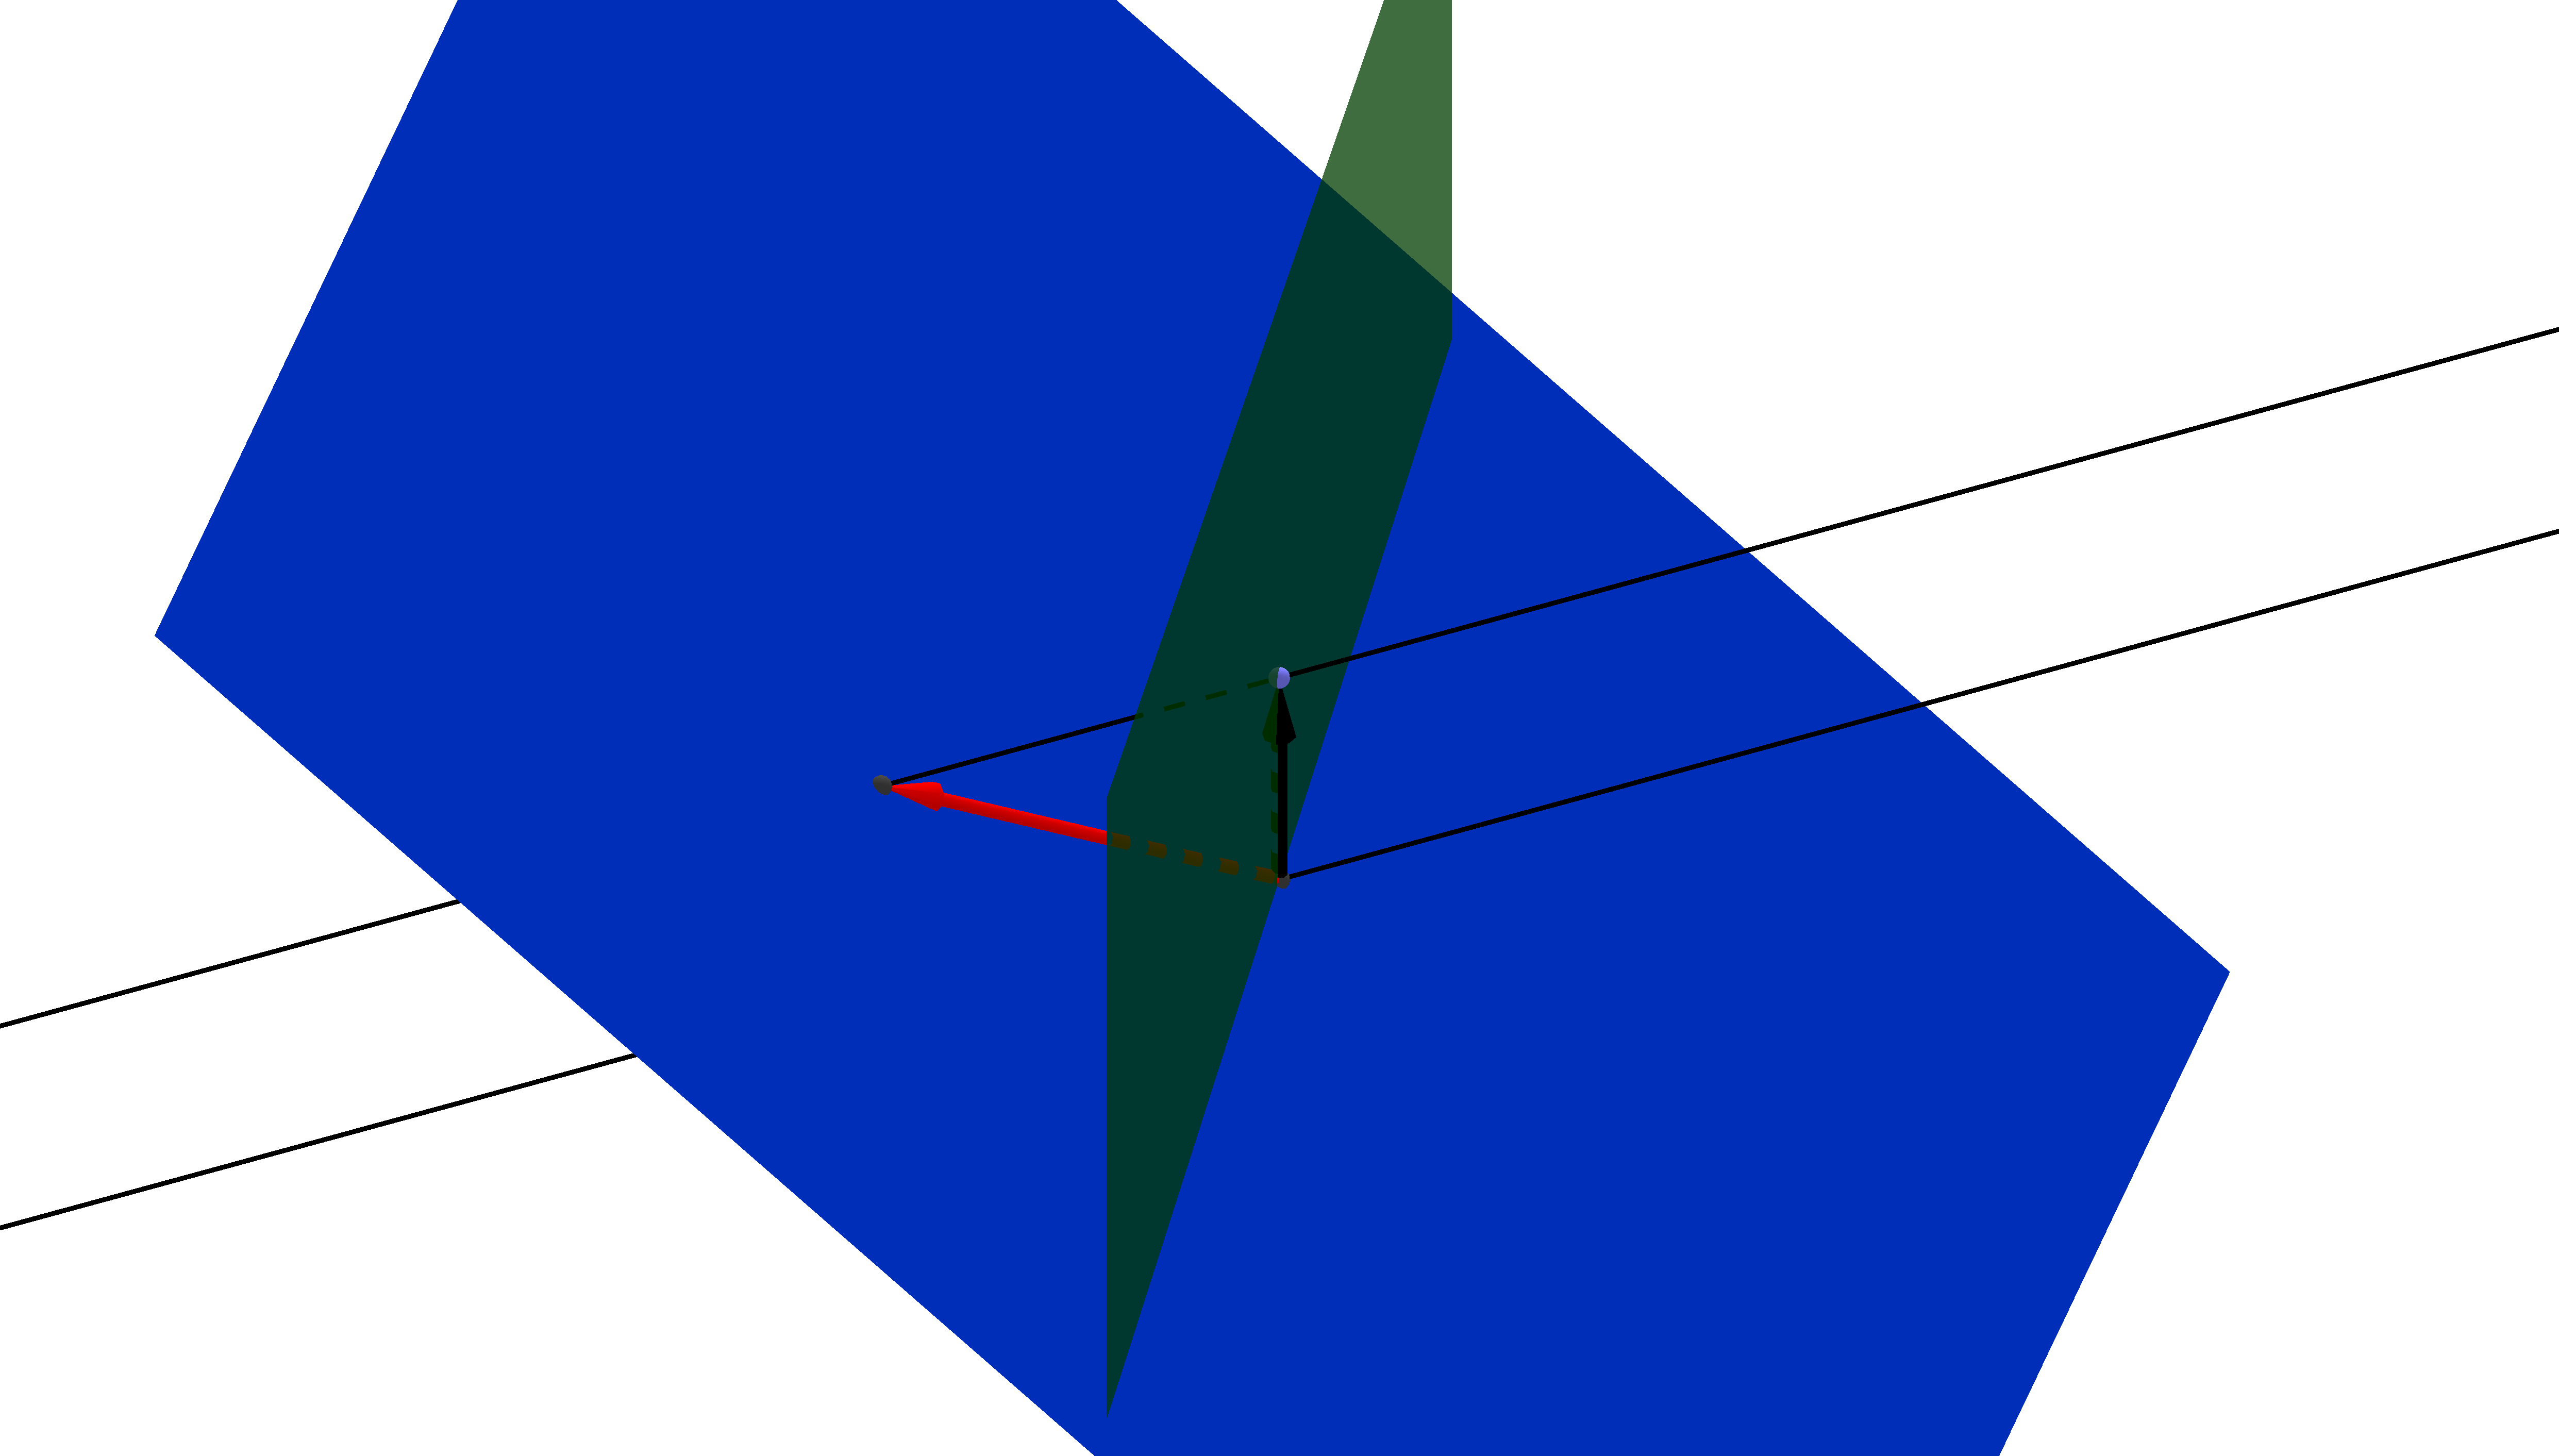
\includegraphics[width=1.0\linewidth]{figures/prop.png}
\caption{The projection matrix will relate the change in residual (black vector) in global XY plane to local XY plane (Blue plane). The propagation must take into account the change in track position intersection. The black lines are the track propagated to the new position.}
\label{fig:Prop}
\end{figure}
 
GBL expects a link which goes from global to local and this defines the parameters used above. You can define the slopes in the local frame and axis in global frame and then invert the corresponding matrix. Either or will work.

The errors associated in the local frame need not be diagonal and will be transformed internally to a frame in which they are. However they must be correct for each measurement. This is simple in most cases were each measurement is independent of position in the local frame. This is true for most strip and pixel sensors but not all. A simple example being a strip sensor with radial strips. This would require that each position has a different error matrix associated with it. Since each strip is oriented differently to the local Cartesian grid which defines the local frame. This situation highlights the difference between the local frame and measurement frame which is often discussed in literature. The measurement frame in one in which the errors are diagonal. Therefore for this example each strips orientation would require a different measurement frame. This requirement has been considered and can be easily added to the measurement function which adds this information.



\subsection{Add scattering information}
\label{sec:scat}
Scattering in the EUTelescope framework is always assumed to be thin (Discussed later). Furthermore the scattering error will non be diagonal in the local frame of the sensor. The propagation matrix from the frame parallel to the track and local frame is

\[ 
\frac{\theta_{0}^{2}}{1-c^2_1 c^2_2}
\left(
  \begin{array}{cc}
 1-c^{2}_{2} & c_{1}c_{2}    \\
 c_{1}c_{2} & 1-c^{2}_{1} \\   
\end{array} \right)\] 



This propagation is shown by \ref{fig:ScatFrame} with the plane perpendicular to the track containing the diagonal error matrix. However if the matrix is transformed to the plane frame (Blue plane \ref{fig:ScatFrame}) then the error matrix will be non diagonal.

\begin{figure}[H]
\centering
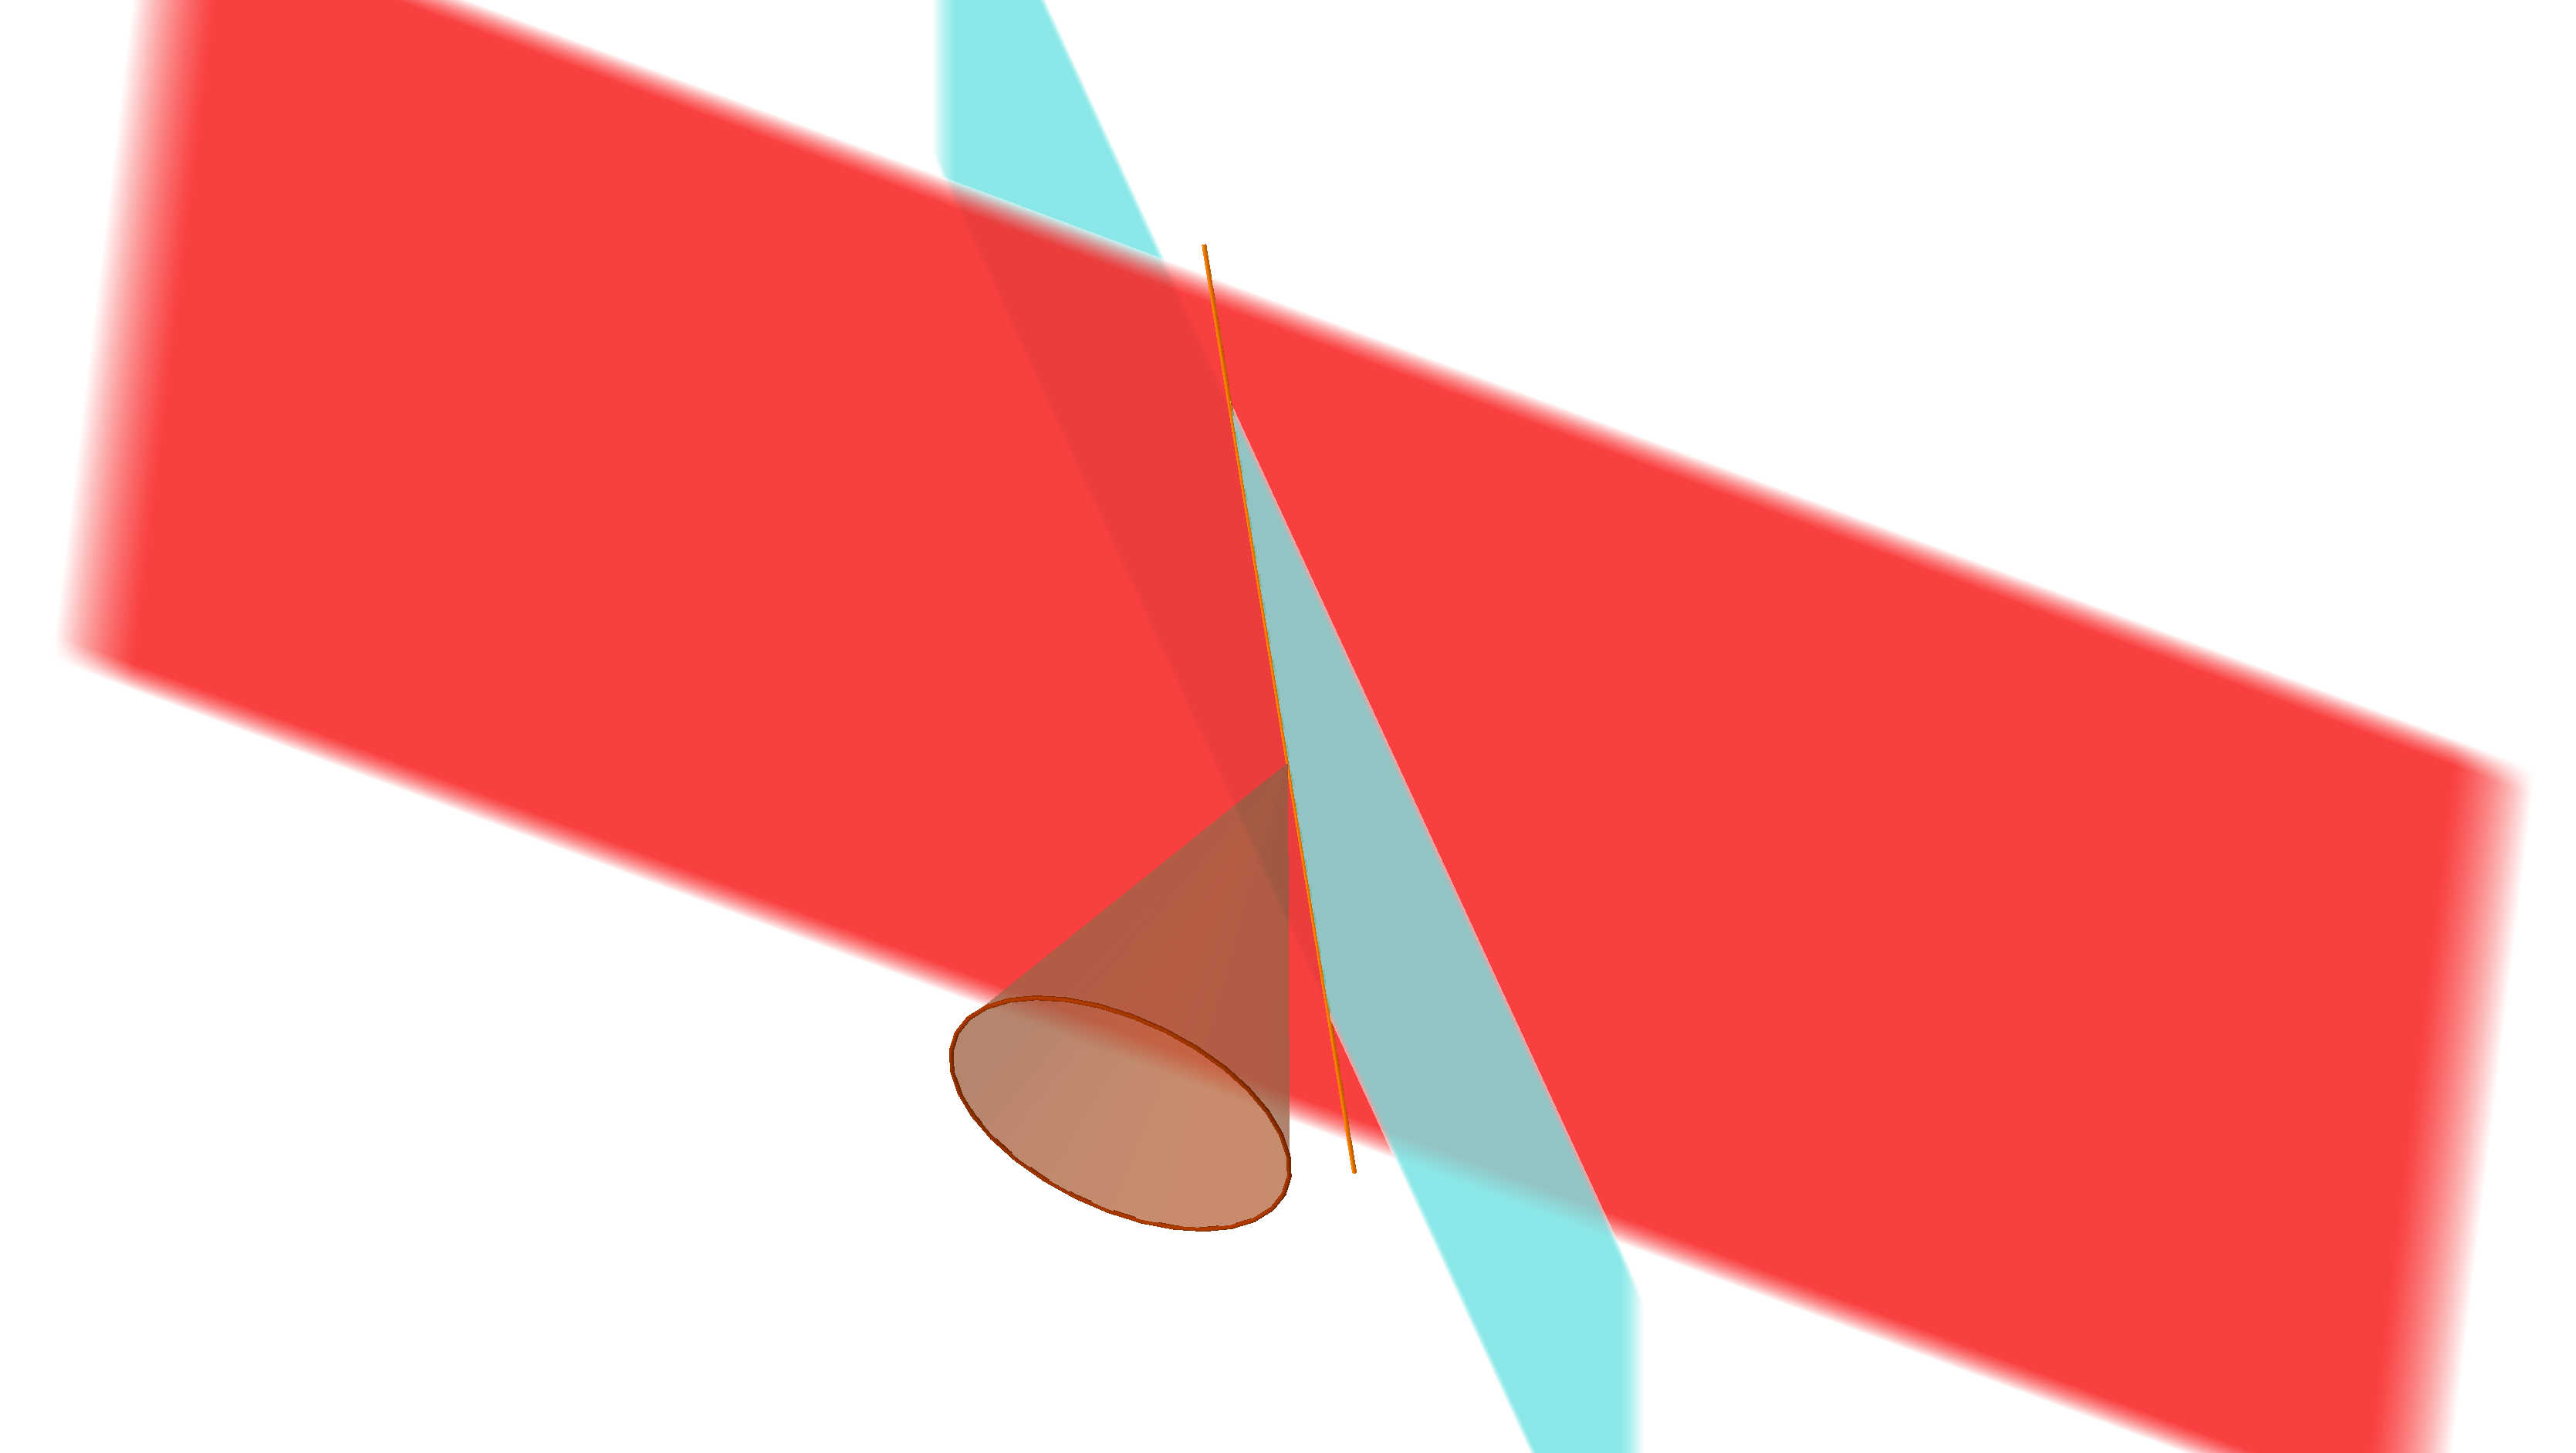
\includegraphics[width=1.0\linewidth]{figures/propGood600.png}
\caption{The scattering frame is the red plane which is perpendicular to the track. The blue plane is the sensor surface. Compare the circular cone which has a diagonal error matrix to the ellipsoid which is non diagonal. This ellipsoid is better seen if the XY plane is propagated downstream with the errors \ref{fig:ScatFrame1}.}
\label{fig:ScatFrame}
\end{figure}

The view of the errors associated from scattering on the plane is shown in figures \ref{fig:ScatFrame1} and \ref{fig:ScatFrame2}. 

\begin{figure}[H]
\centering
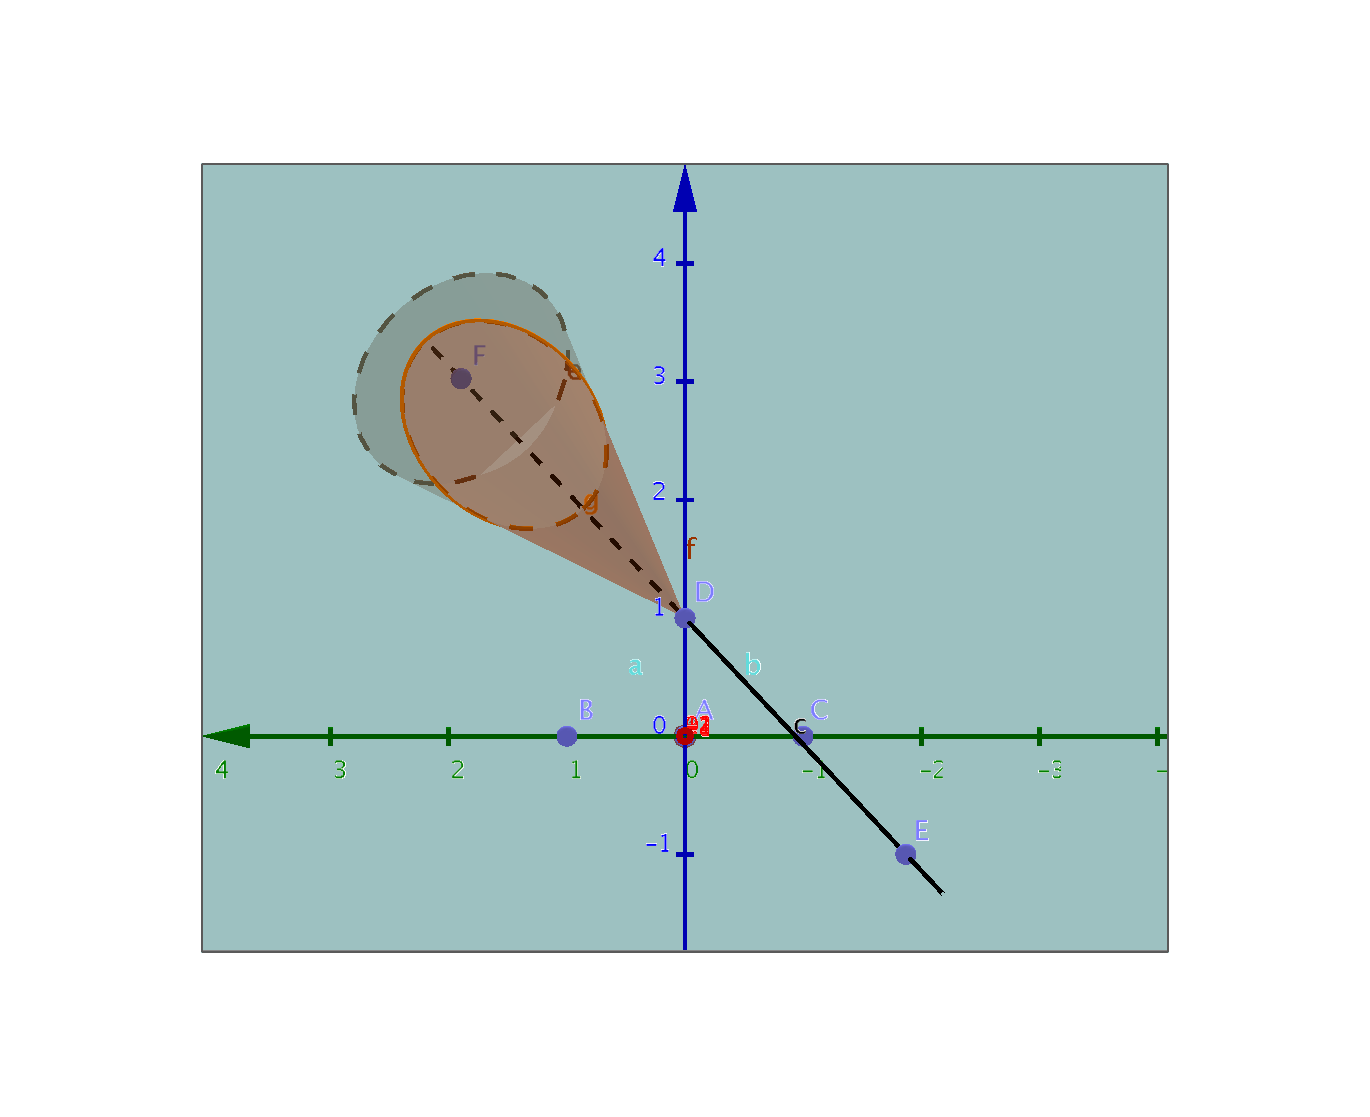
\includegraphics[width=1.0\linewidth]{figures/scatterDownZProjection.png}
\caption{The scattering cone projected on the XY plane of the sensor. The errors on the sensor must take this form to propagate correctly in the z axis}
\label{fig:ScatFrame1}
\end{figure}

\begin{figure}[H]
\centering
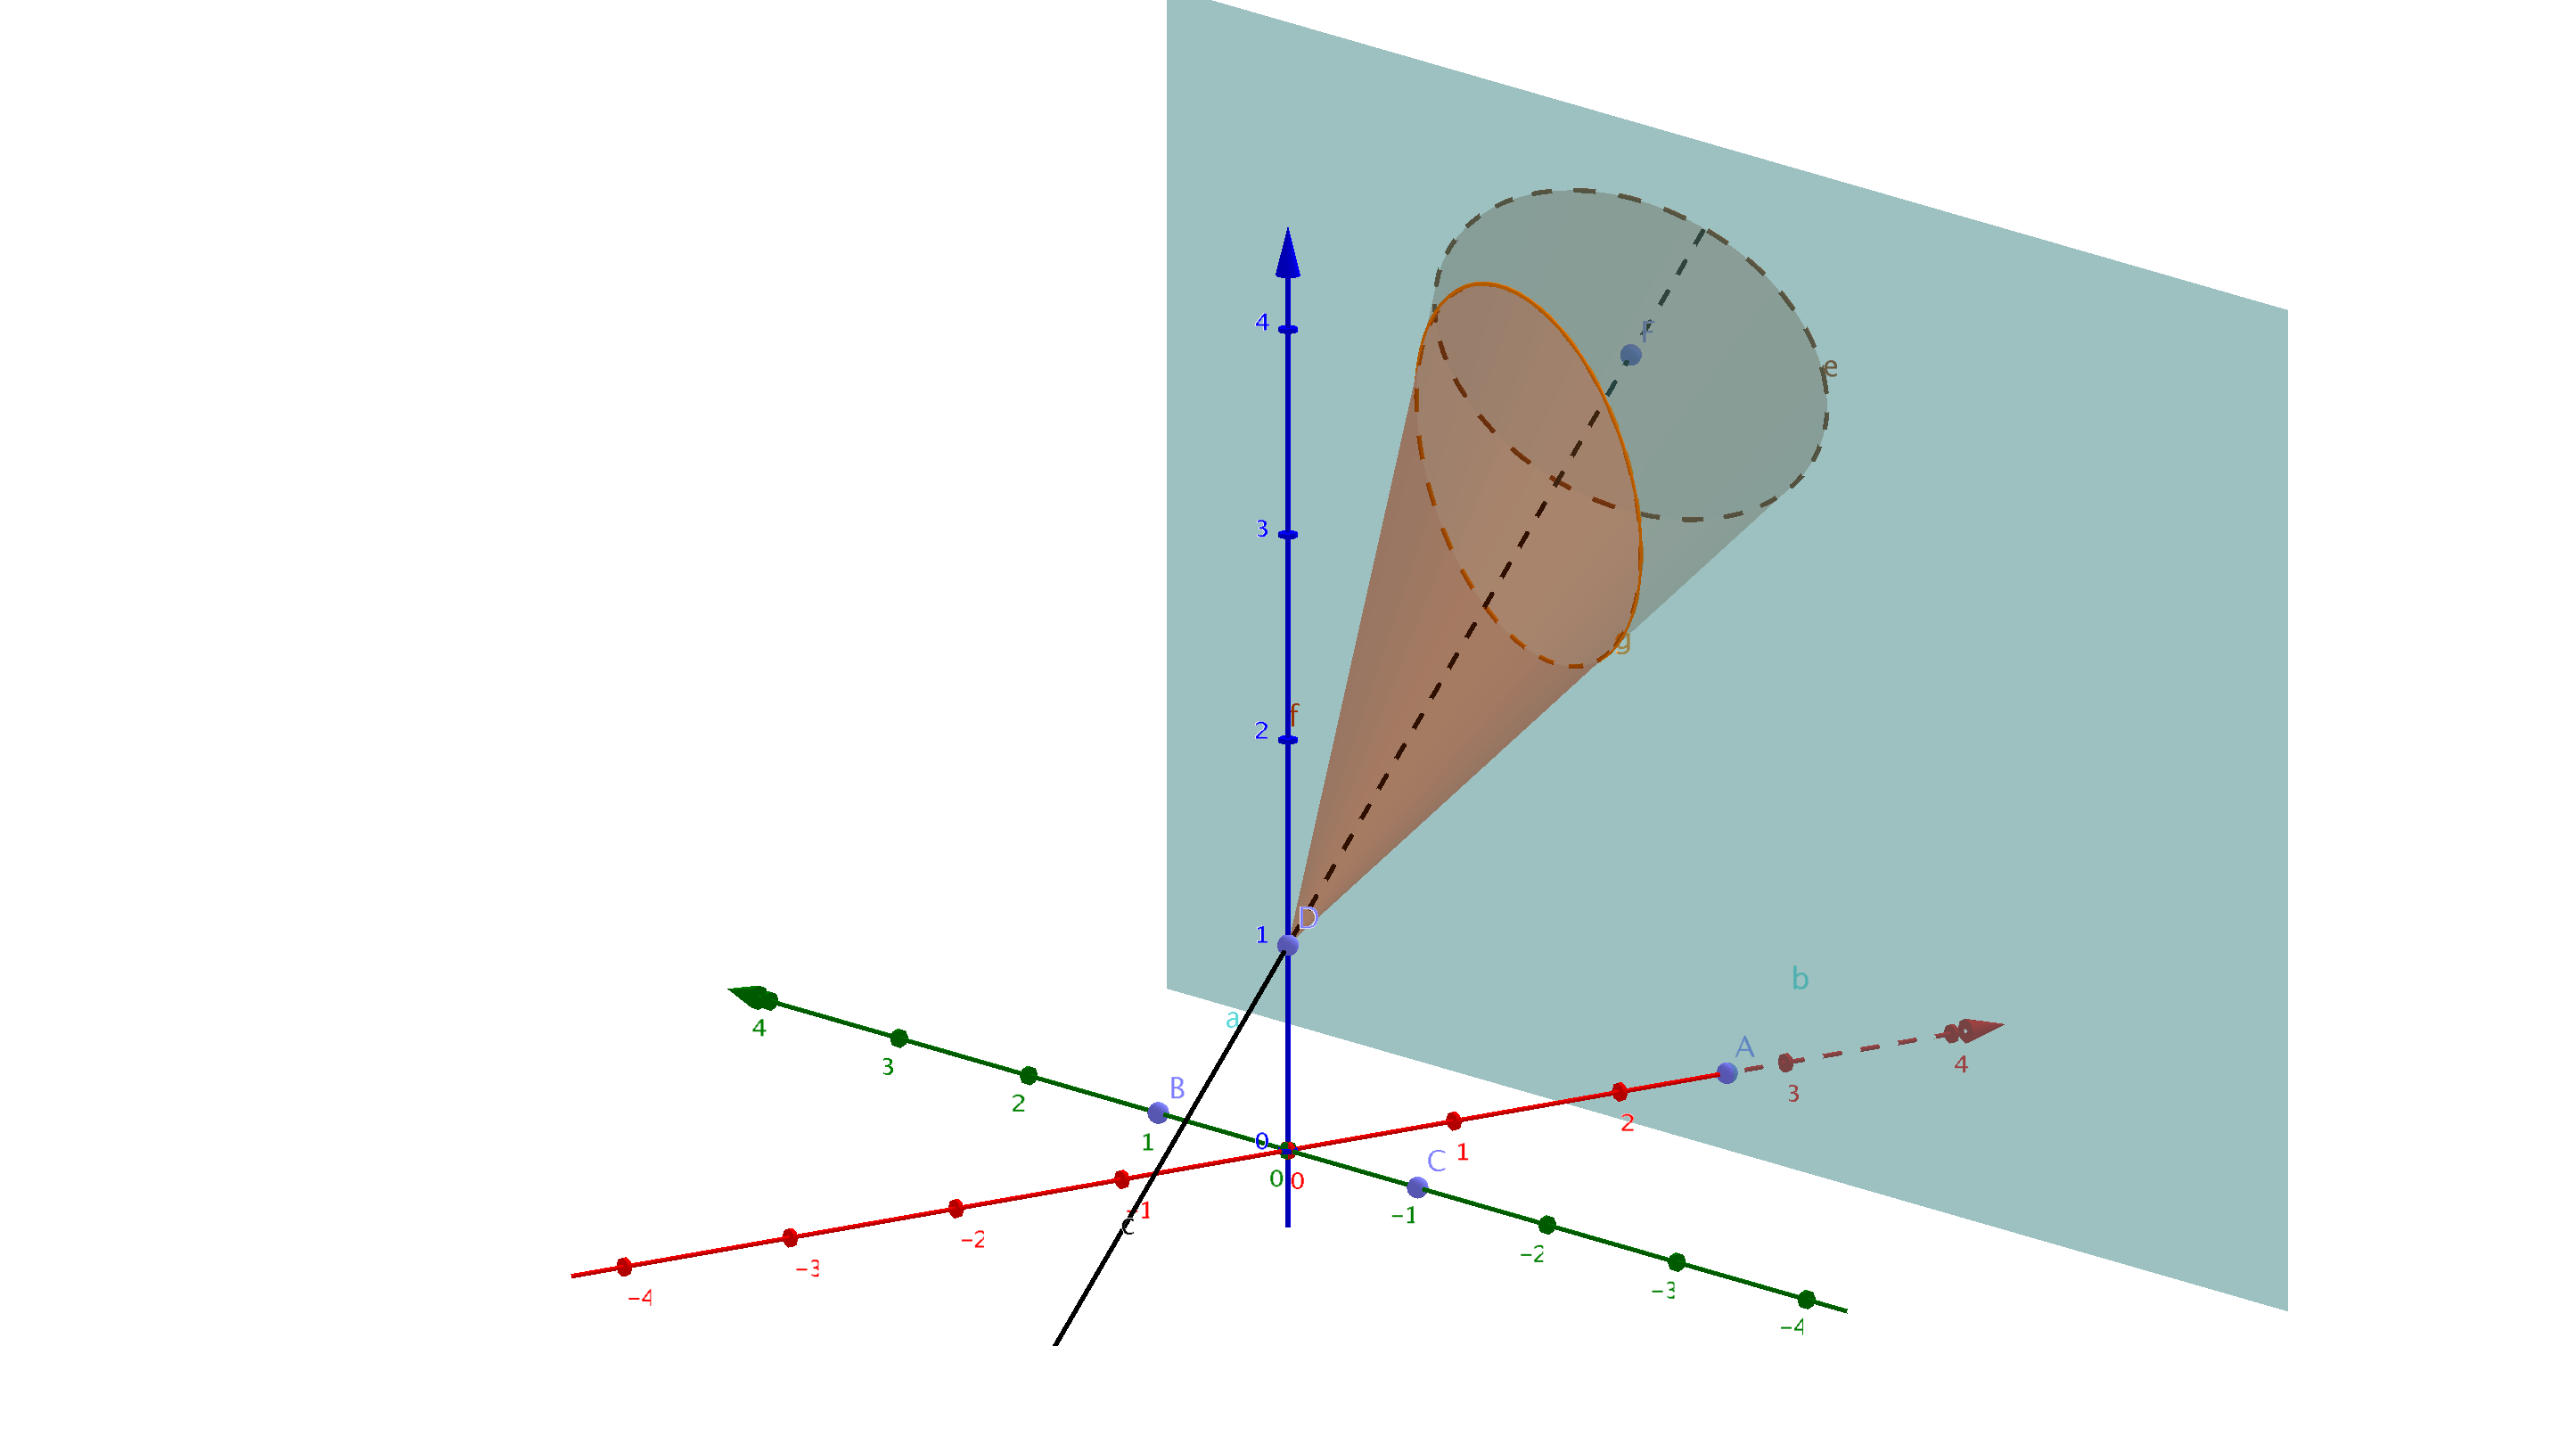
\includegraphics[width=1.0\linewidth]{figures/prop600GoodOffSensor.png}
\caption{The same as figure \ref{fig:ScatFrame1} from a different angle.}
\label{fig:ScatFrame2}
\end{figure}

The propagation of scattering errors to different frames is all well and good. However you must be able to determine the amount of scattering expected at each point.

First the total radiation length must be determined for the track's trajectory. TGeo volumes are used to describe the full detector system including the radiation length. The track is assumed to propagate through each volume at the appropriate incidence to determine the correct radiation length at each point. Two things must be determined to model scattering.

First the variance at each point must be determined. To determine this the total variance of the trajectory must be calculated. The total variance is calculated using the radiation length and beam energy. This is were the Highland formula comes in. The Highland formula relates the radiation length percentage and beam energy to a scattering RMS. One important characteristic of the Highland formula is its non linear properties: The radiation length calculated must be for the full system and then split between each point used to model the scattering. 

Second the position of the scatterers must be determined. This depends on the radiation length and size of the volume to model. If the volume is thin then it can be assumed a thin scatterer. A thin scatter will have no displacement through the material but some angular displacement. So all the radiation length is located at that point. The red measurement dots on figure \ref{fig:LinkJac} are modeled this way. The variance at this point is the total variance weighted by the fraction of radiation length at this point relative to the total radiation length.
A thick scatterer will have some displacement due to scattering within the material and can be viewed as the combination of many thin scatterers. If you propagate the error associated with each thin scatterer which makes up the thick scatter then it can be shown that a thick scatterer can be modeled by two thin scatterers. The location and allowed variance of the kinks is determined using the relations

\begin{multicols}{2}
\begin{equation}
 s_1 = s_0
\end{equation}
\begin{equation}
s_2 = \overline{s} + \frac{\Delta s^{2}}{\overline s - s_1} 
\end{equation}
\begin{equation}
\theta_{1}^{2} = \theta^{2}\frac{\Delta s^{2}}{(\Delta s^2 + (\overline s - s_1)^{2}} 
\end{equation}
\begin{equation}
\theta_{2} = \theta^{2}\frac{(\overline s - s_1)^{2}}{\Delta s^2 + (\overline s - s_1)^2} 
\end{equation}
\end{multicols}

were $\theta^{2}$ is the total variance, $s_0$ as the initial position of the scattering volume and 

\begin{multicols}{3}
\begin{equation}
\theta^{2} = \int_{a}^{b} \theta_{i}^{2}
\end{equation}
\begin{equation}
\overline{s}=\frac{\int_{a}^{b} s_i \theta_{i}^{2}}{\theta^2}
\end{equation}
\begin{equation}
\Delta s^{2} = \frac{\int_{a}^{b} ( s_i  - \overline{s})^2 \theta^{2}_{i}}{\theta^2}
\end{equation}
\end{multicols}

were T=b-a which is the start and end position of the scatterer volume. 
Integration can be used to work out the parameter values for any inhomogeneous volumes. Most situation will have blocks of homogeneous material one after the other. In this case the above equation can be treated as: 

\begin{equation}
 \overline{s} = 0.5 \sum_i \frac{T_i}{X0_i} 
\end{equation}

\begin{equation}
 \Delta s^{2} = \sum_i \frac{\frac{1}{3} T^3 - T^{2}\overline{s} + T\overline{s}^{2}}{X0_i} 
\end{equation}

\begin{equation}
 norm =   \frac{T_i}{X0_i} 
\end{equation}

were T is the thickness and the summation is over all homogeneous volumes.  This allows the correct modeling of the radiation length for the full particles trajectory. 

If a more detailed radiation length calculation is needed then the tracks actual trajectory through the full TGeo volumes space can be used. However in all examples this is not required. Care must be taken that the TGeo volumes described contain the sensor hits. Since a transformation between local and global can move the hits outside these volumes. The current simple radiation length calculations do not suffer from the this problem since they always travel through each blocks' centre.

Dead material which should be added as radiation length but is of no interest is identified in the gear file with $ID>99$. One example in section \ref{example} demonstrates this.



\subsection{Add global parameters}
\label{gloPar}
The addition of global parameters is used to determine alignment corrections. However this can be used for any variables which are common to all tracks. Note this in contrast to local parameters which vary from track to track.  Alignment is simply the determination of the correct transformation from local to global frames for each sensor. 

\begin{figure}[H]
\centering
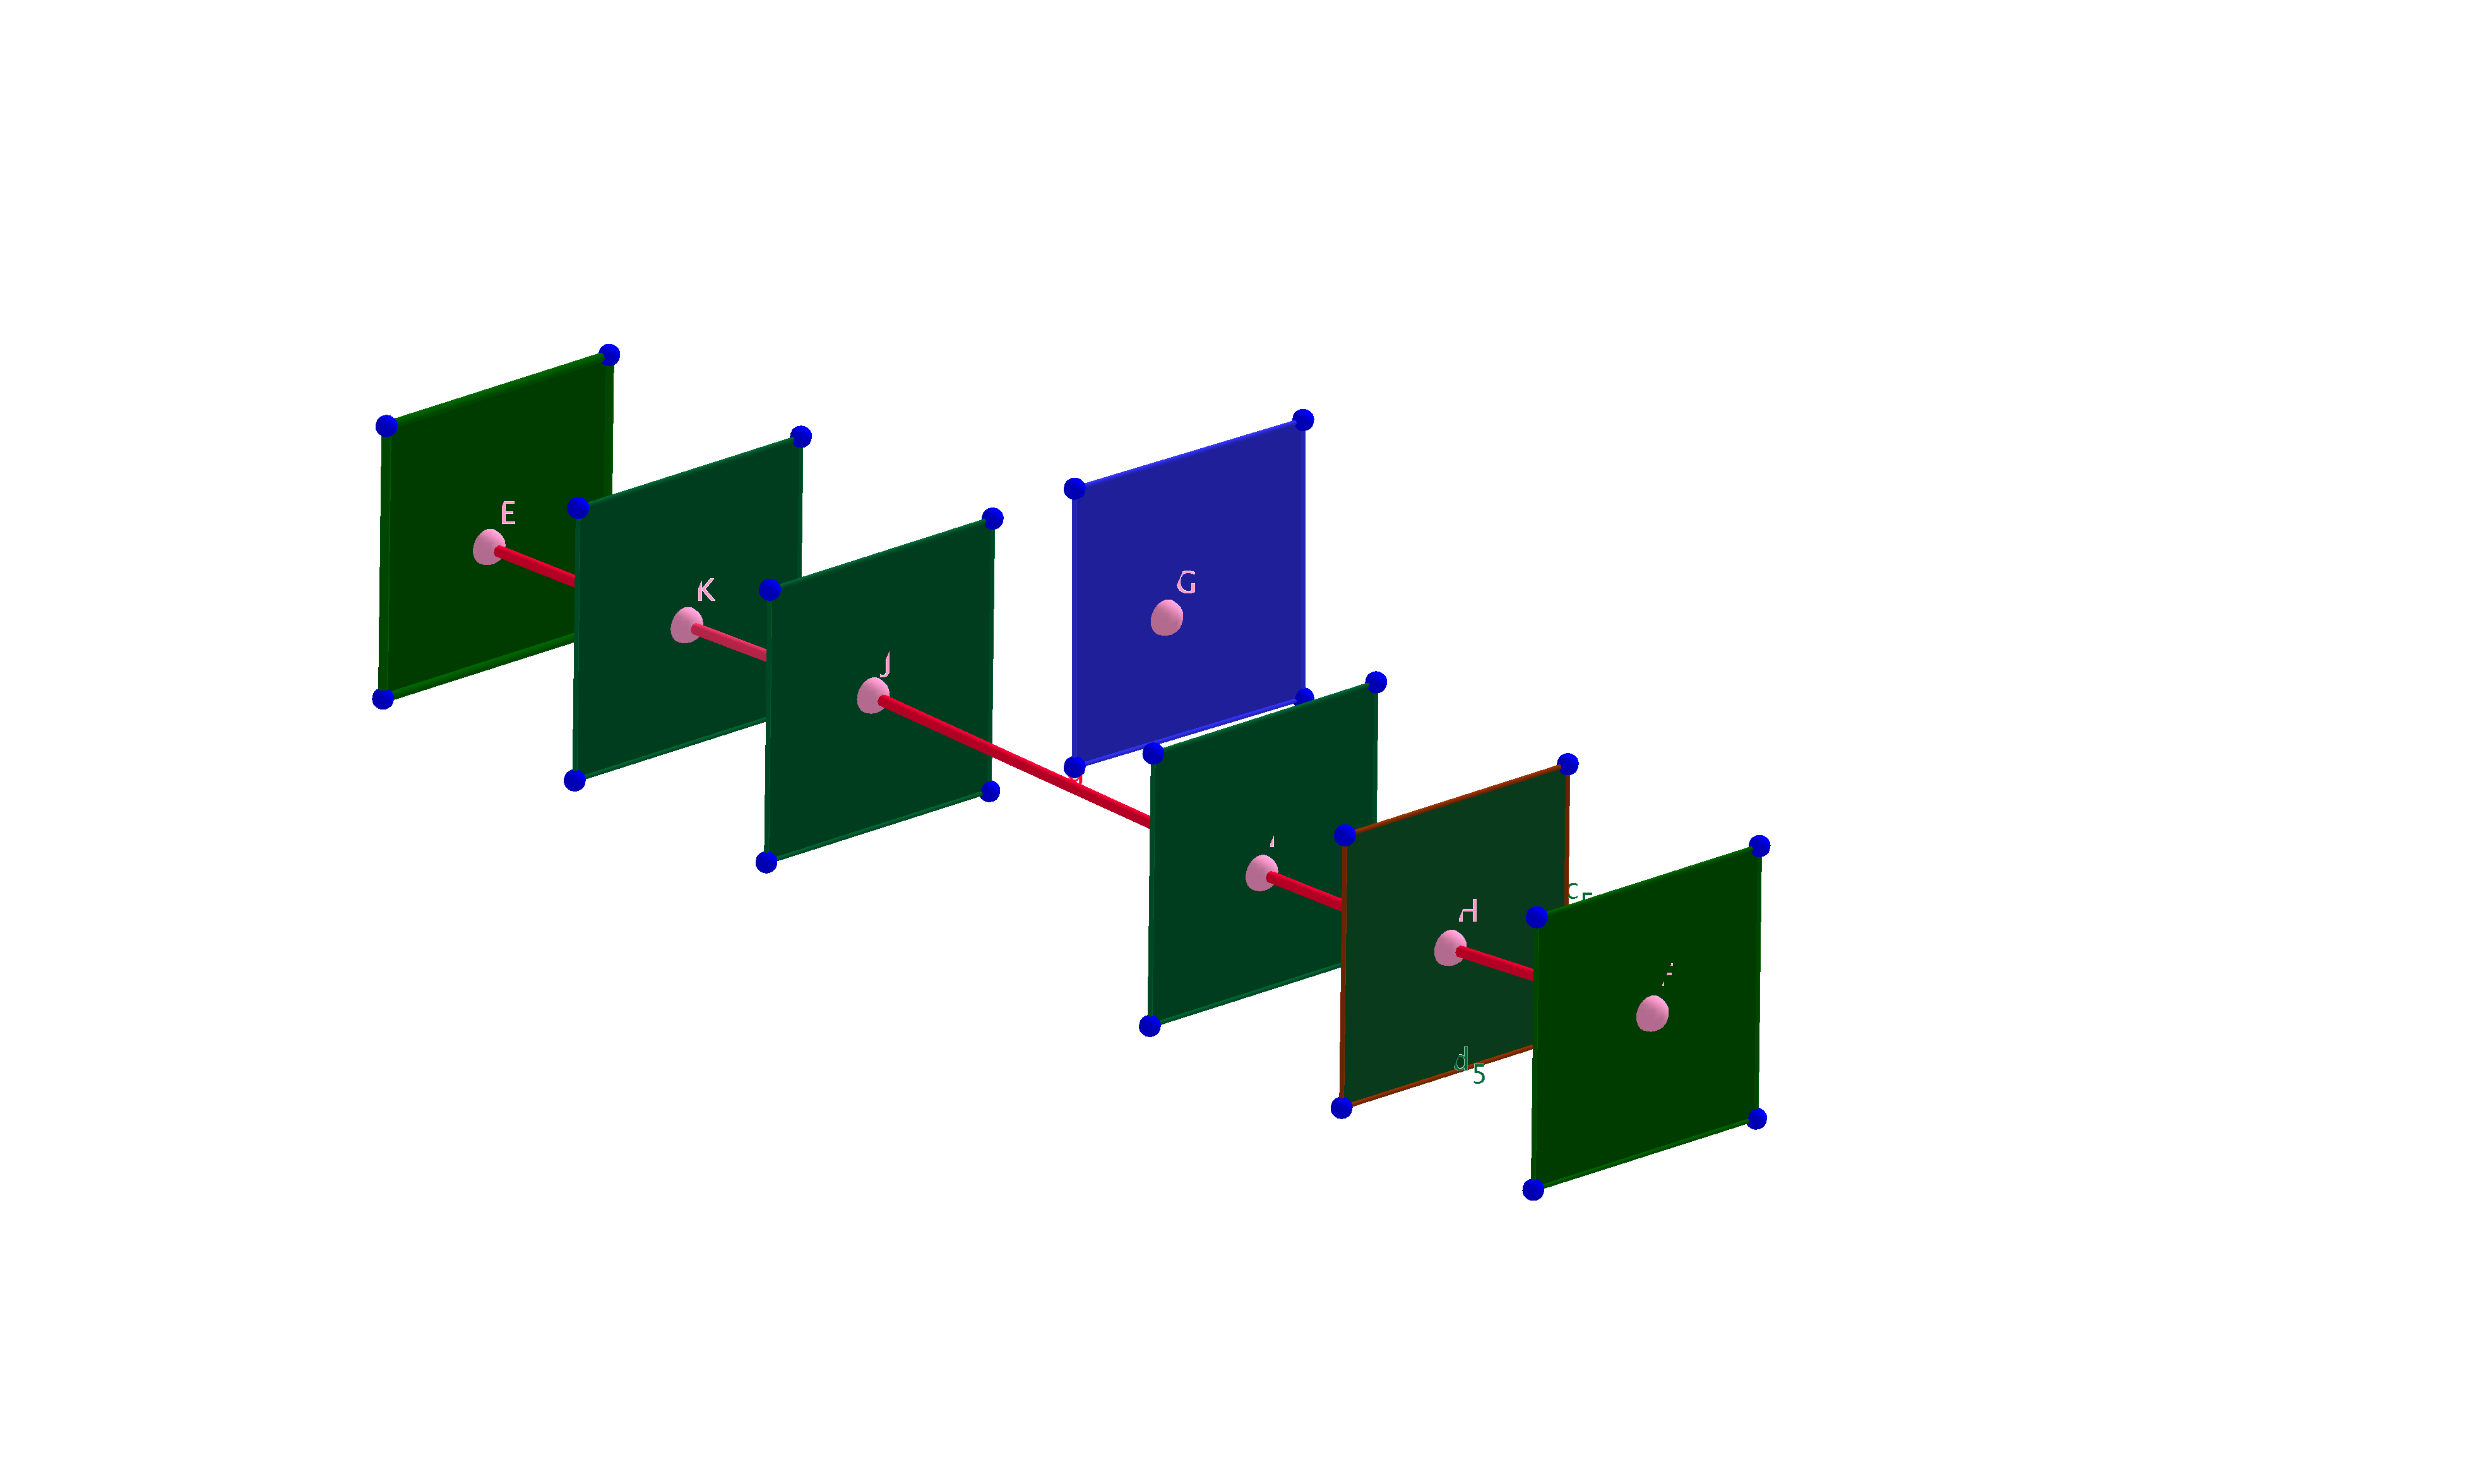
\includegraphics[width=1.0\linewidth]{figures/MisAlignStraight.png}
\caption{Illustration of misalignment with DUT. The transformation of the local DUT frame to the global frame must be wrong so the corrections must be found.}
\label{fig:MisAlign}
\end{figure}

Figure \ref{fig:MisAlign} illustrates a clear problem with the description of the sensor in space. The corrections needed are assumed to be the transformation between global and local frames which minimizes the residual weighted with errors for all tracks and planes.

A link between the local frame residual and alignment parameters which define the transformations must be determined. The alignment parameters are defined $(X,Y,Z, \alpha,\beta,\gamma)$ which are the offsets in the global frame and the rotations defined in each frame of the rotations applied before it. This last point is important: The corrections to the rotations must be determined in the frame reached before that rotation is applied. So the $R_X$ (Rotation round X axis) matrix correction must be determined after you have rotated round the Z axis. This can be dealt with in two ways: 

1) Determine the corrections for each rotation in the frame it is applied then rotate to the local frame. 

2) Only apply large rotations and parity transforms before you apply corrections. 

The second approach is taken with all X/Y rotations applied in the initial rotation matrix. Note rotation round the Z axis is also permissible since this is the first matrix to be corrected. The parameters' change is related to change in position of a point in the coordinate system by the  \emph{point correction matrix} $\hat{PC}(X,Y,Z, \alpha,\beta,\gamma)$:
\[ \left( \begin{array}{cccccc}
1 & 0 & 0 & 0 & relZ & -relY \\
0 & 1 & 0 & -relZ & 0 & relX  \\
0 & 0 & 1 & relY & -relX & 0   
  \label{eq:PC}
\end{array}
 \right)\] 

This matrix will create a correction vector at the location and coordinate system specified by the relative positions. 
The relative positions are defined as the global predicted position without offsets. This is done so the order of magnitude of the rotation is correct. So defined as:

\begin{equation}
 \overrightarrow{rel} =   \hat{R}\overrightarrow{L} 
\end{equation}

The predicted positions used are the pattern recognition tracks and not the GBL fit.  

\begin{figure}[H]
\centering
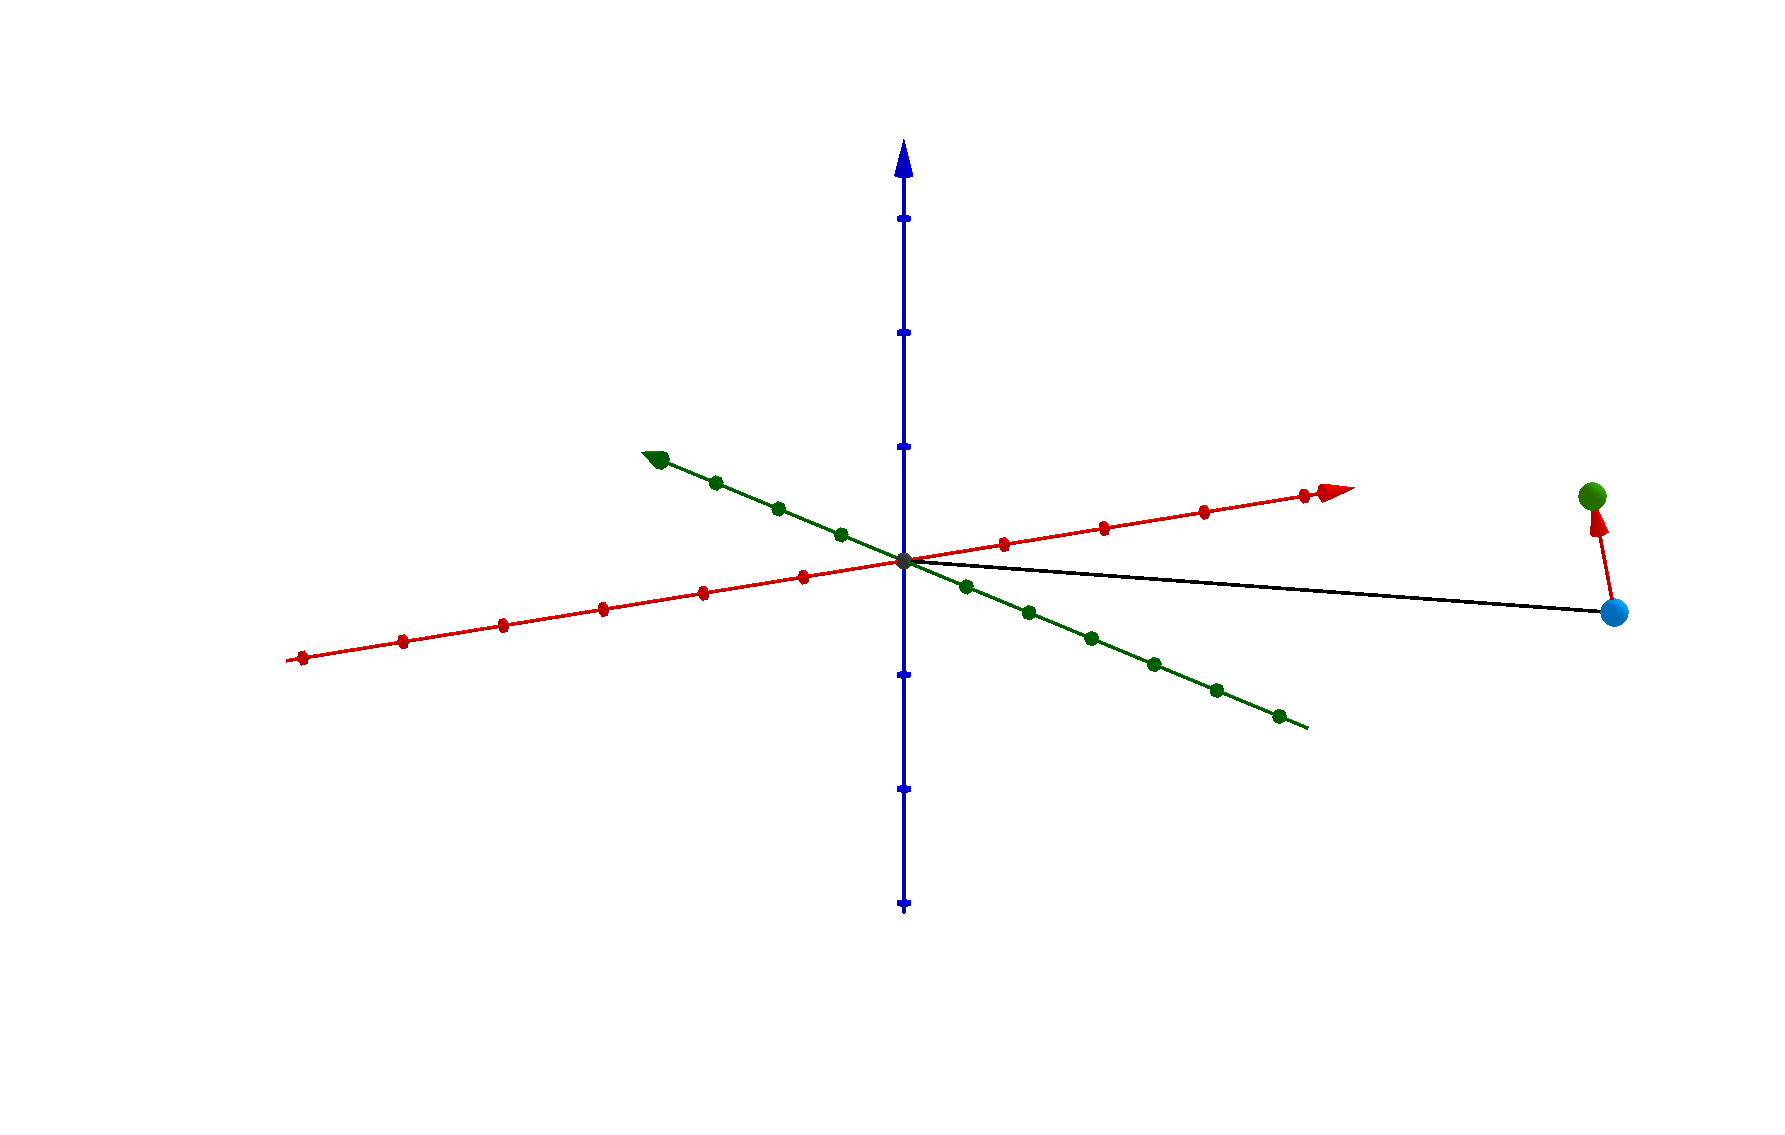
\includegraphics[width=1.0\linewidth]{figures/corrAlign.png}
\caption{The point correction matrix for a particular relative position. The vector is the correction to apply to this point given a certain $(X,Y,Z, \alpha,\beta,\gamma)$ change in the coordinate system.}
\label{fig:CorrMatrix}
\end{figure}

The correction vector will not give the change measured on the plane from moving the track. To estimate this the correction vector must be considered moving a track rather than a point. This is done using the \emph{track correction matrix} $\hat{TC}(\overrightarrow d, \overrightarrow n )$ 
\begin{equation}
  I -  \frac{\overrightarrow d \times \overrightarrow n}{\overrightarrow d . \overrightarrow n}\\
  \label{eq:TC}
\end{equation}

which will move a track by a particular displacement and determine how this changes the intersection with a plane. 

\begin{figure}[H]
\centering
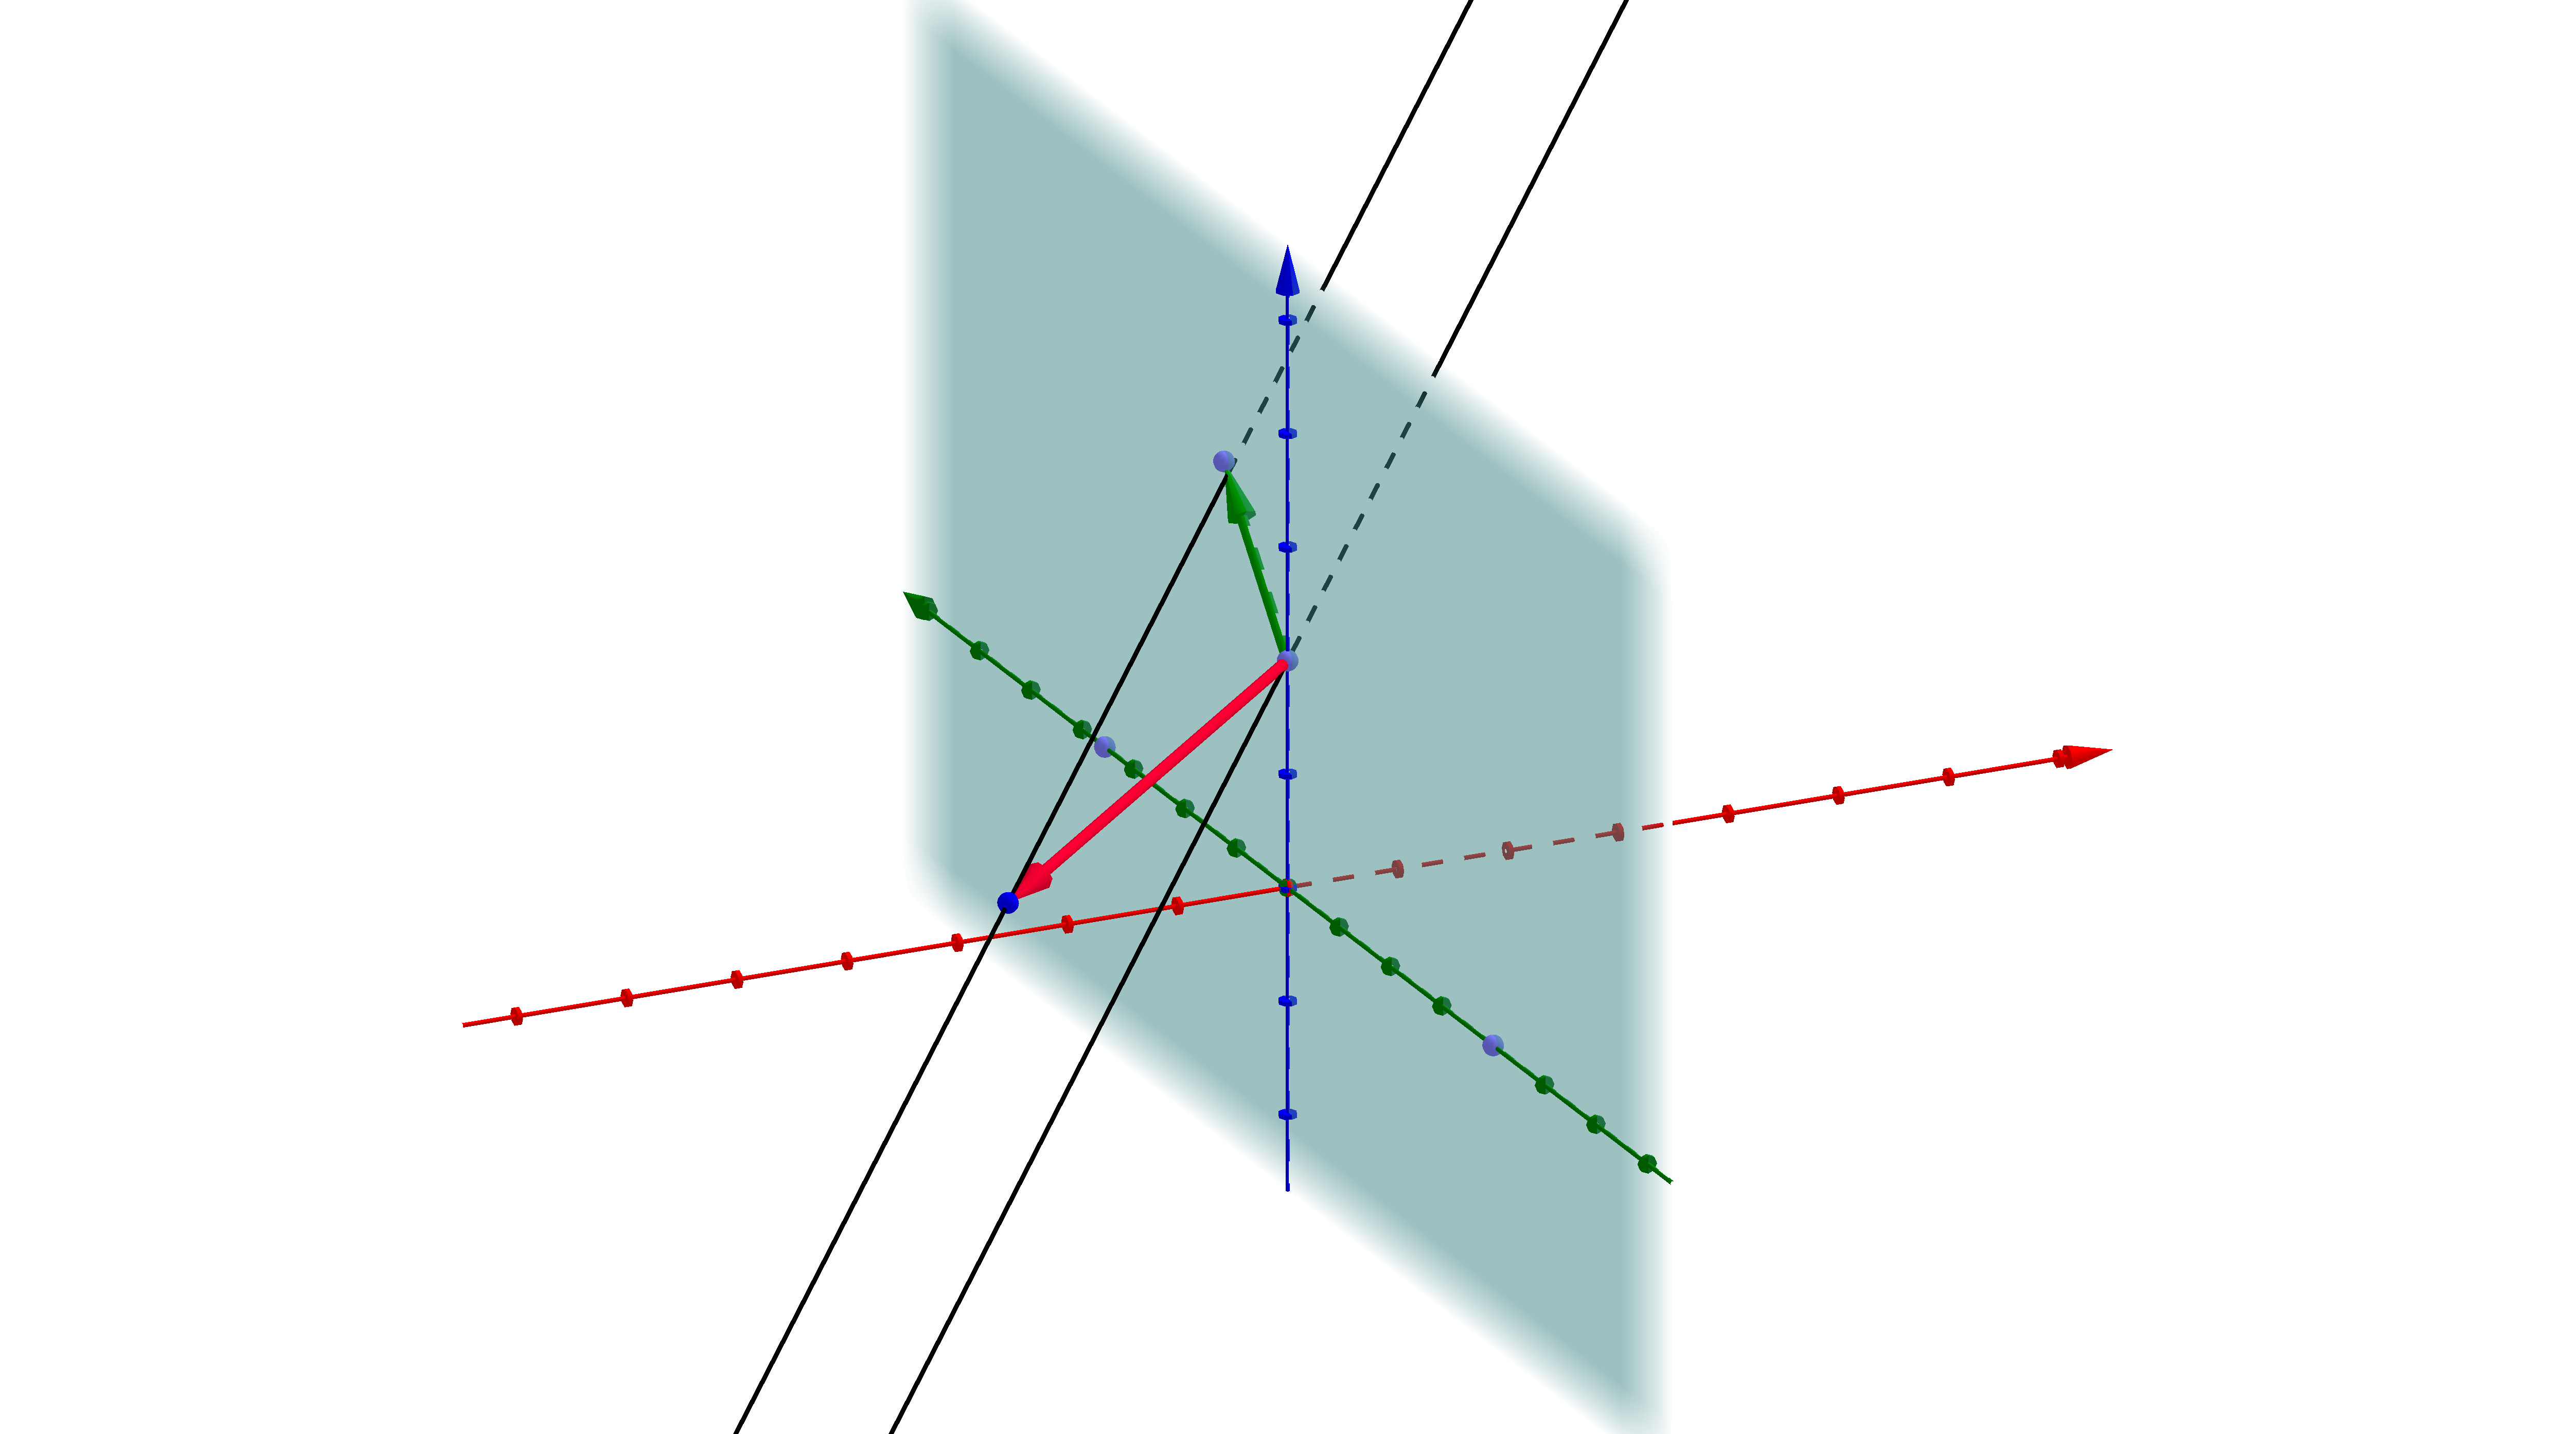
\includegraphics[width=1.0\linewidth]{figures/alignBigger.png}
\caption{The track correction matrix will take as input the track displacement given in red. It will then determine the green vector which is the change on the plane due to that displacement}
\label{fig:TC1}
\end{figure}

\begin{figure}[H]
\centering
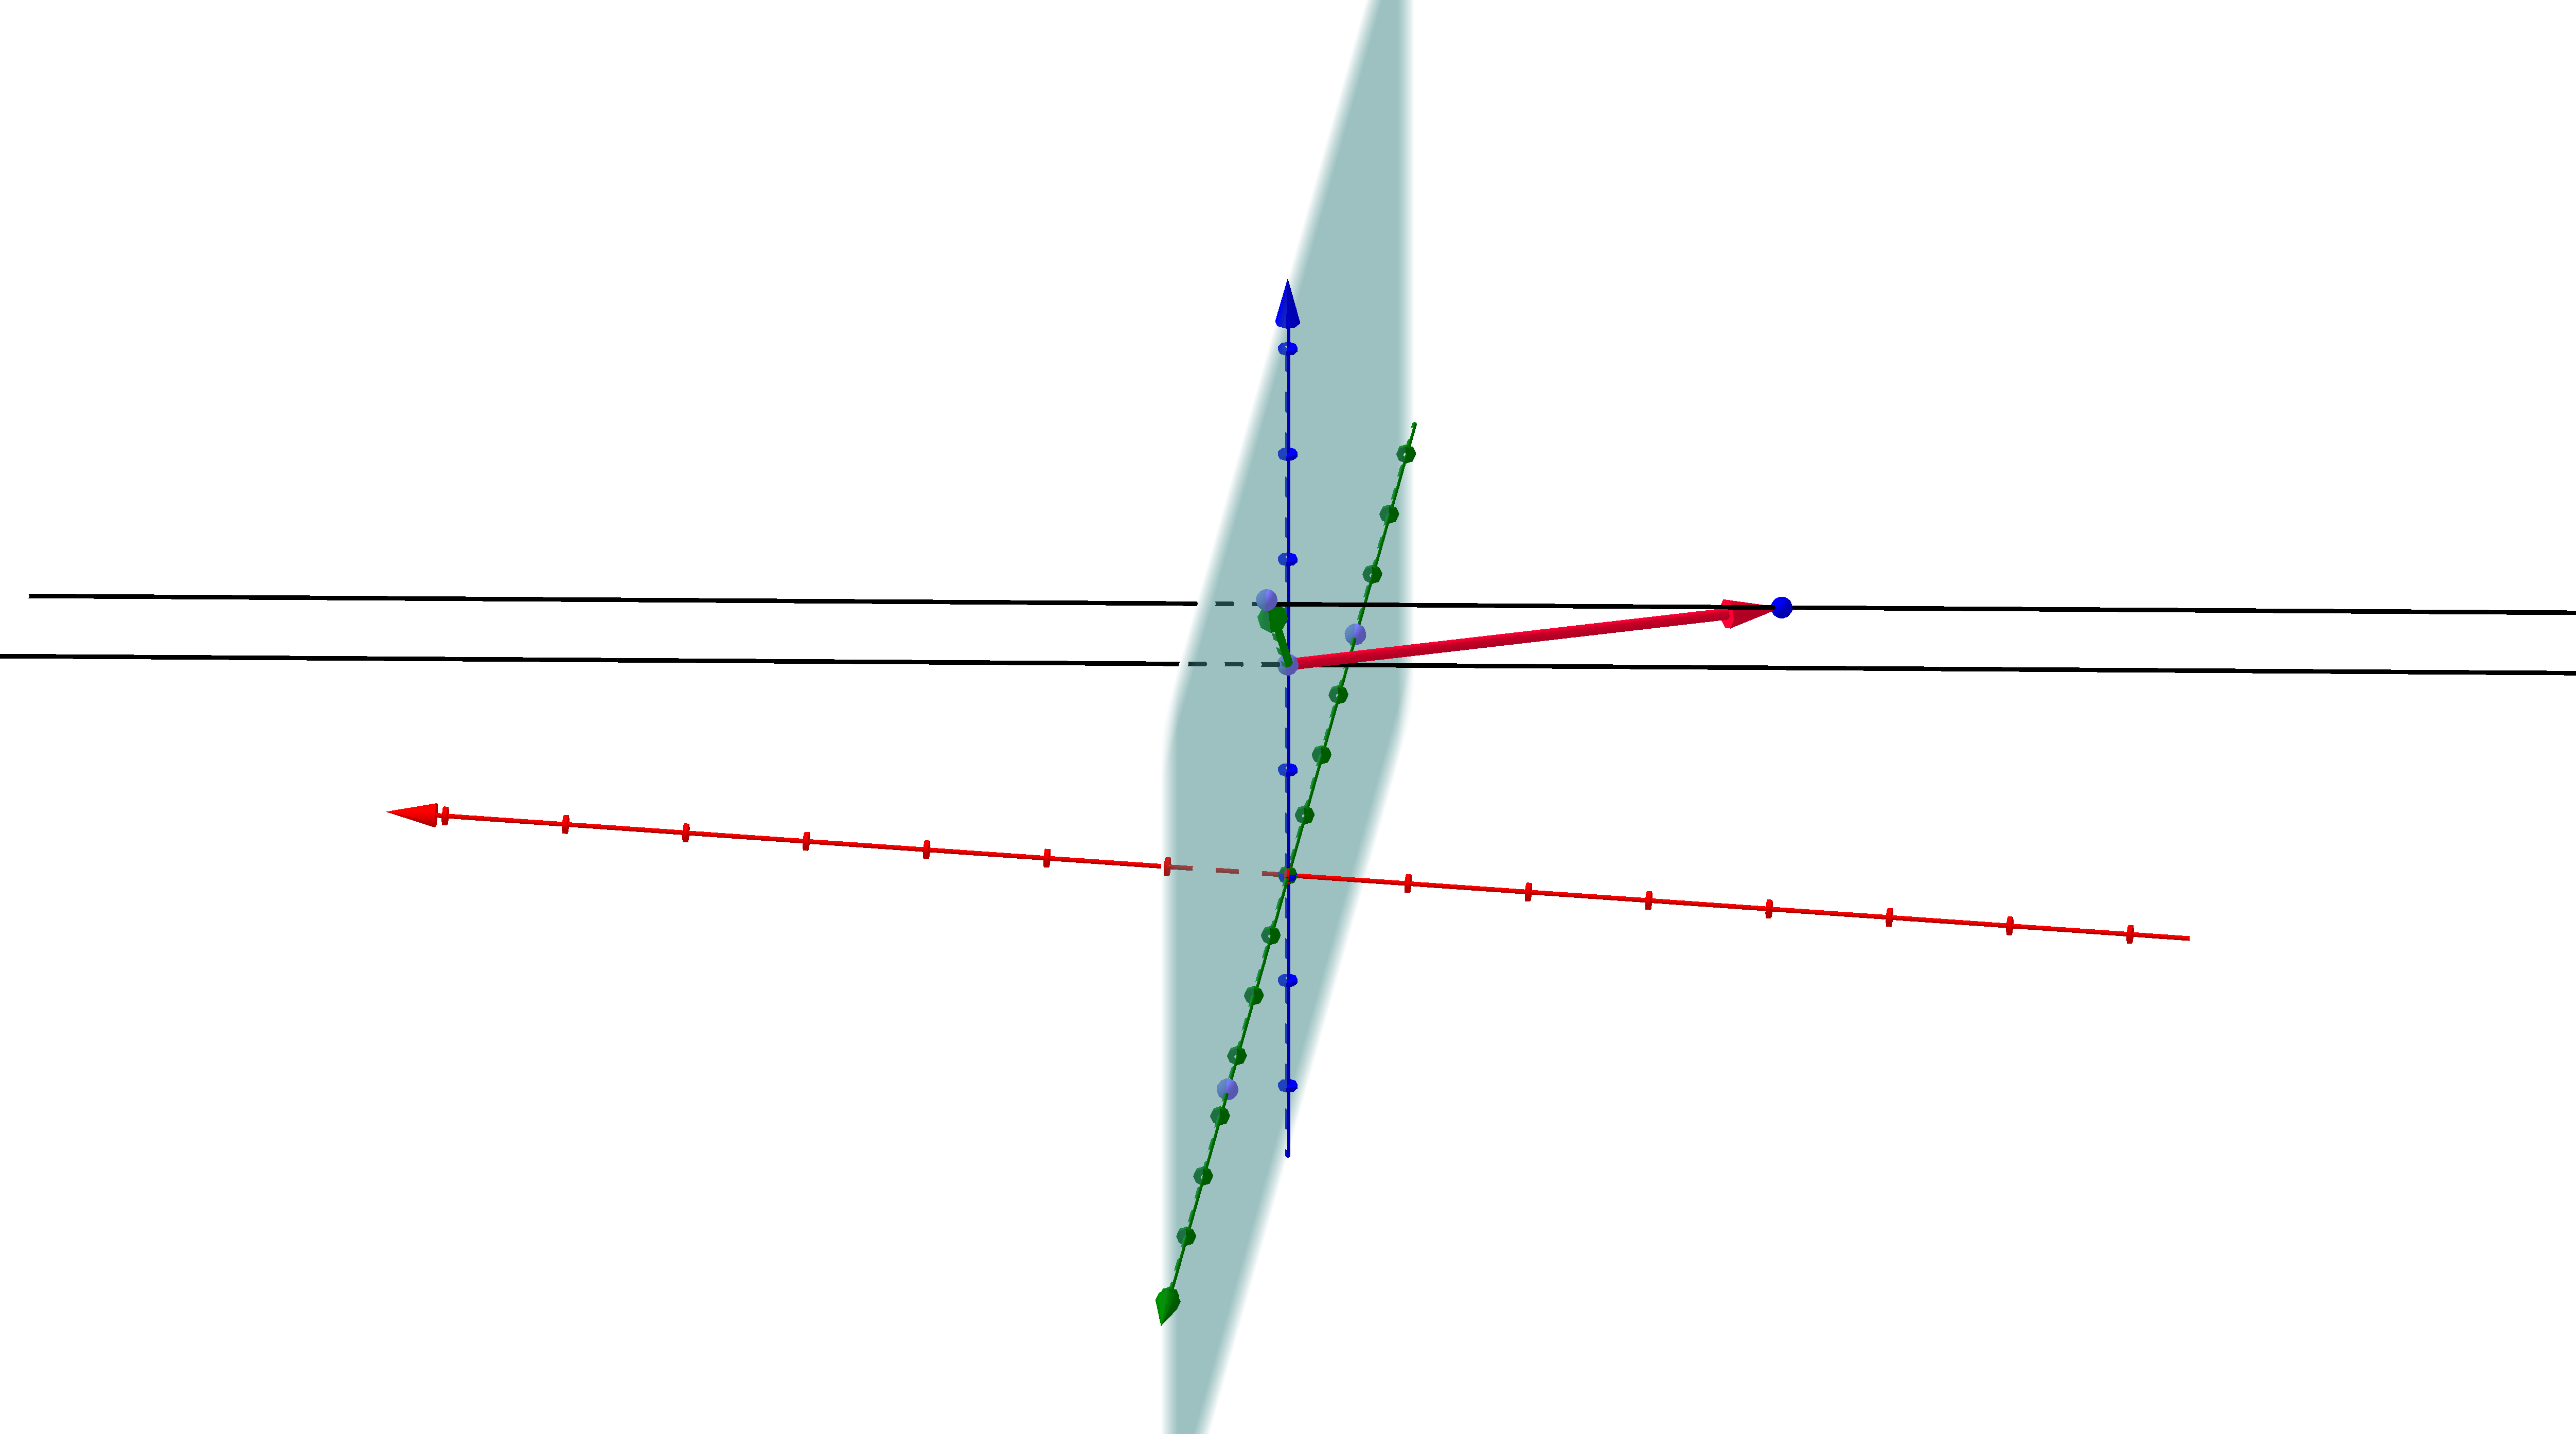
\includegraphics[width=1.0\linewidth]{figures/alignmentBigger.png}
\caption{Same as \ref{fig:TC1} but from a different angle. The green vector is on the plane surface.}
\label{fig:TC2}
\end{figure}

The final full body alignment can determined by combining TC and PC. This will relate the change in global alignment parameters to change on a plane. The plane described is in the global frame. Therefore the vector on the plane must be rotated into the local frame of the sensor. This frame will of course have zero Z displacement since it should be on the sensor surface. The final matrix passed to millepede:

\begin{equation}
\hat{R^{T}} \hat{TC} \hat{PC} 
\end{equation}

were the transpose of the rotation matrix is the inverse.

\subsection{Add local parameters}

Local parameters are added in the same way as global. However the variables of interest will vary from track to track. Local parameters have been added to the software to determine kink angles at a particular point.

Kink angles can be estimated using the plane ID=271 in the gear file at any detector position. This method could be used to determine the radiation length of the detector system in the future. However it is only in the initial stages of development and should be used with caution.

%
%
%\subsection{Quad}
%
%The Quad module (250x50) is placed in the centre of the setup with a reference DUT. Both are aligned and have comparable resolutions. The Quad module residual is shown in figure \ref{fig:quad}. The resolution in Y is larger than expected. This has been a common theme with all FEI4 devices and has been demonstrated with DAFFitter. 
%
%\begin{figure}[H]
%\hspace{-35mm}
%\subfloat{\label{fig:beamE5B1} 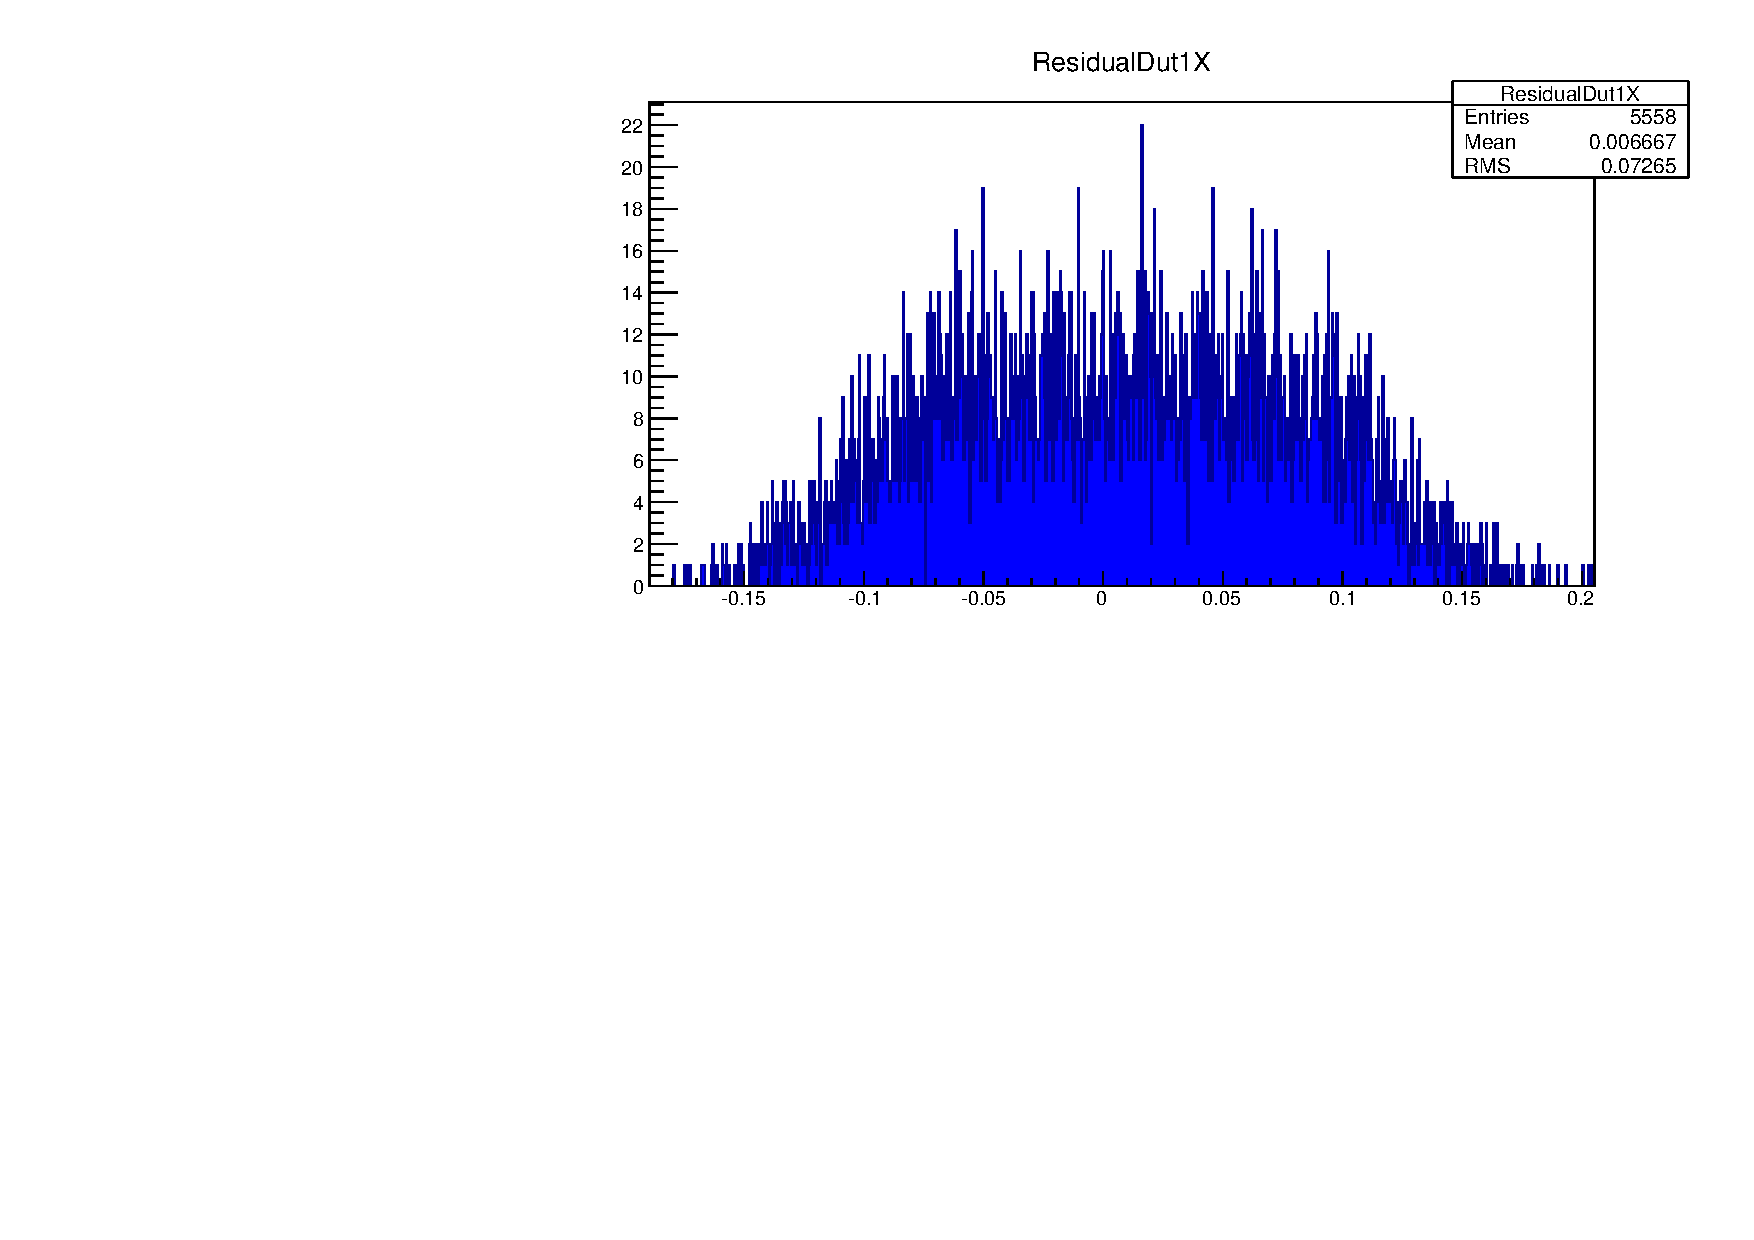
\includegraphics[scale=0.5]{figures/QuadXRes21.pdf}}
%\subfloat{\label{fig:beamE5B1} 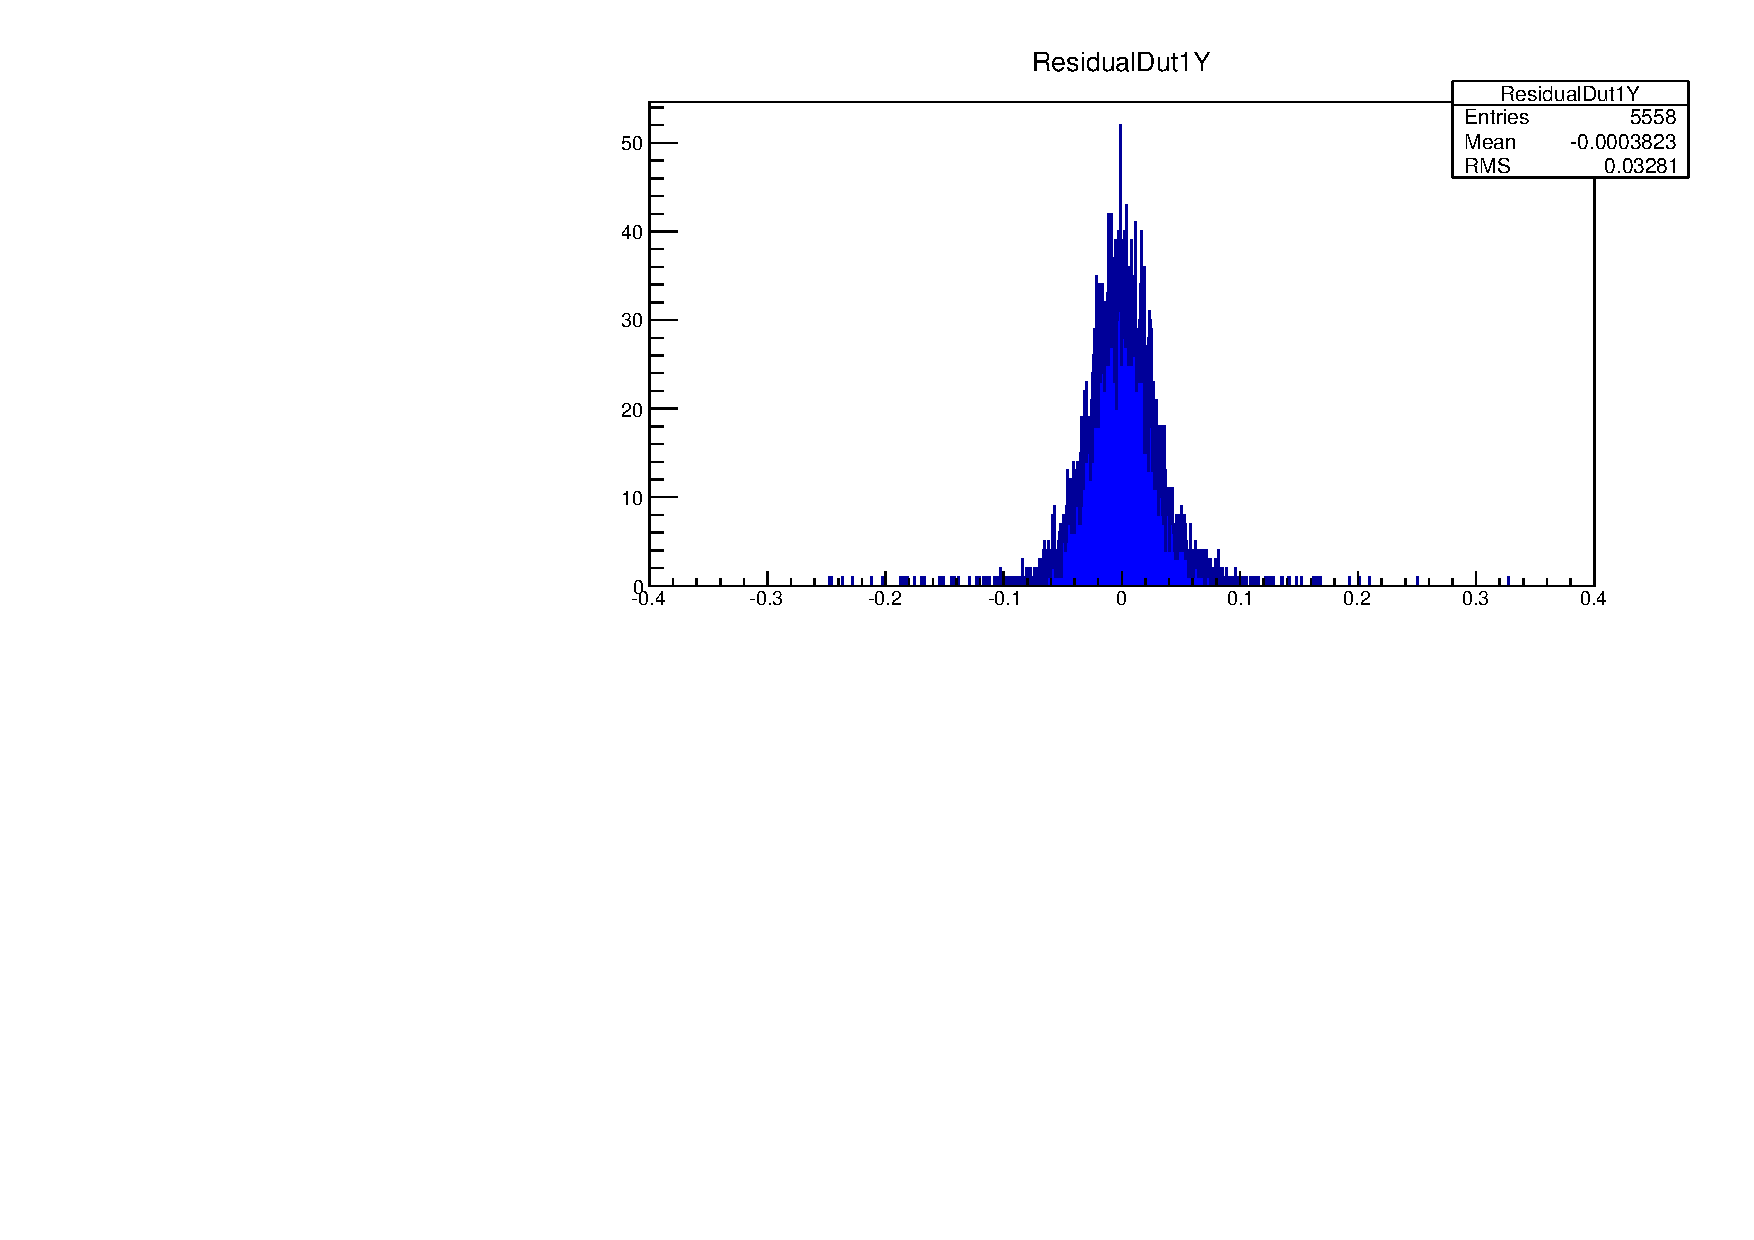
\includegraphics[scale=0.5]{figures/QuadResY.pdf}}
%\caption{ Residual of Quad module in local X/Y axis. }
%\label{fig:quad}
%\end{figure}
%
%\subsection{APIX pixel}
%
%Two APIX pixel DUTs are placed in the beam at DESY. 
%
%\begin{figure}[H]
%\hspace{-35mm}
%\subfloat{\label{fig:beamE5B1} 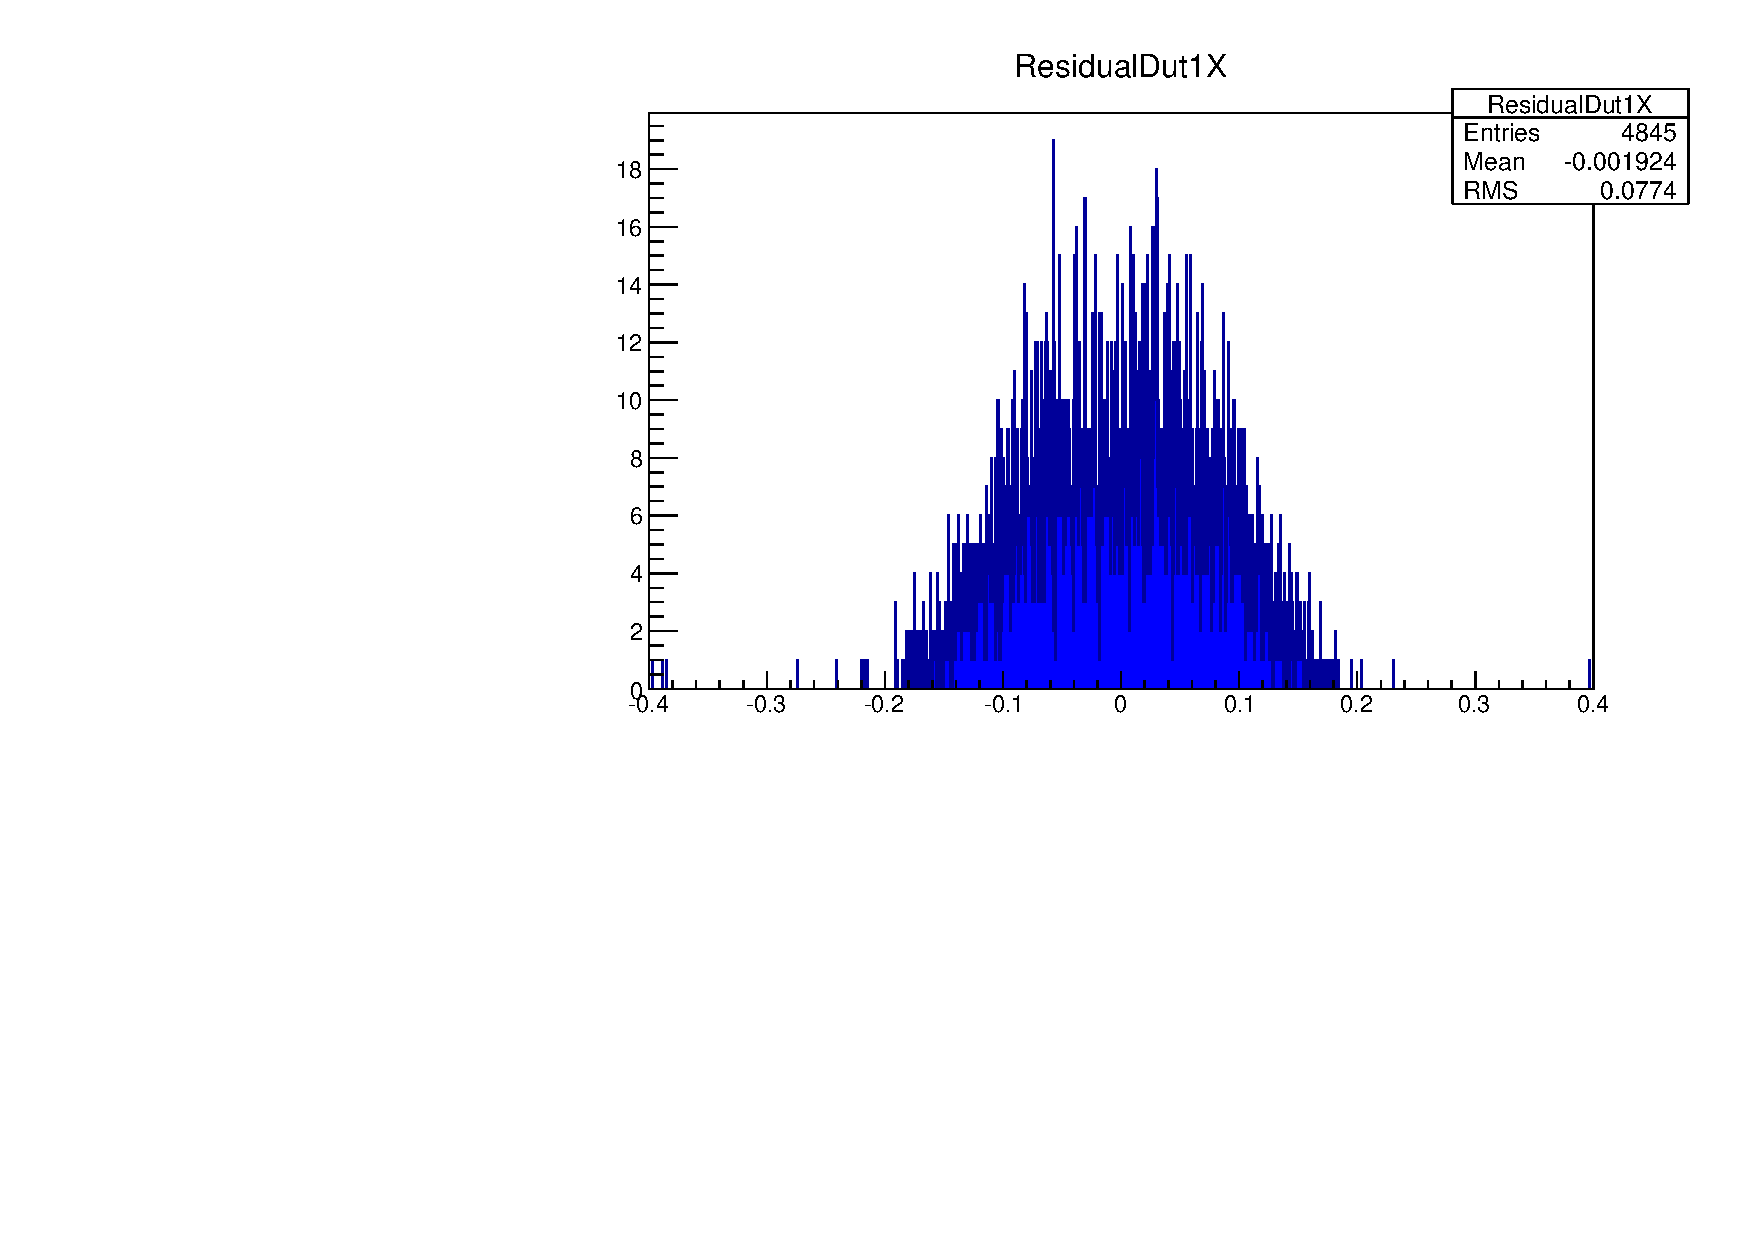
\includegraphics[scale=0.5]{figures/resXpixel.pdf}}
%\subfloat{\label{fig:beamE5B1} 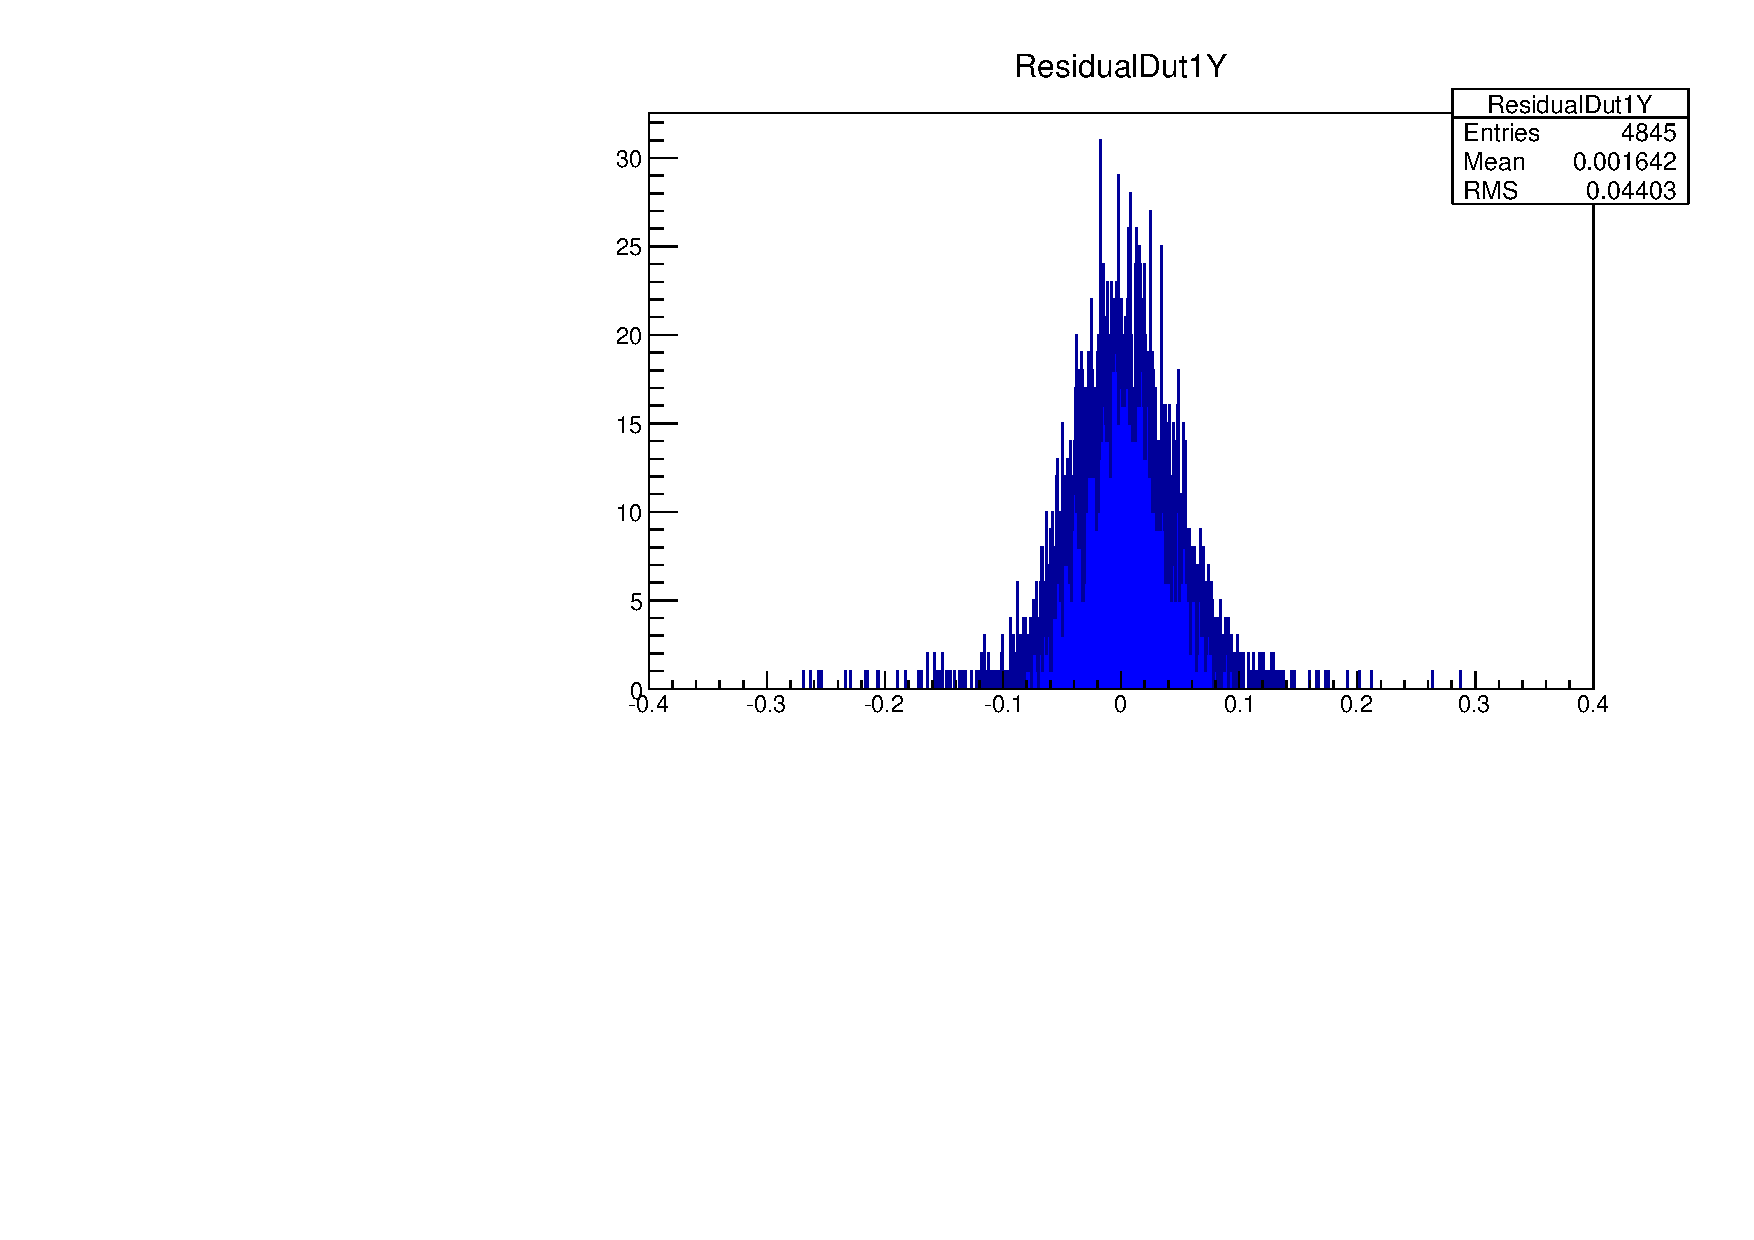
\includegraphics[scale=0.5]{figures/resYpixel.pdf}}
%\caption{The resolution with 10k events on DUT 21. }
%\label{fig:kinkRad}
%\end{figure}
%
%
%\begin{figure}[H]
%\hspace{-35mm}
%\subfloat{\label{fig:beamE5B1} 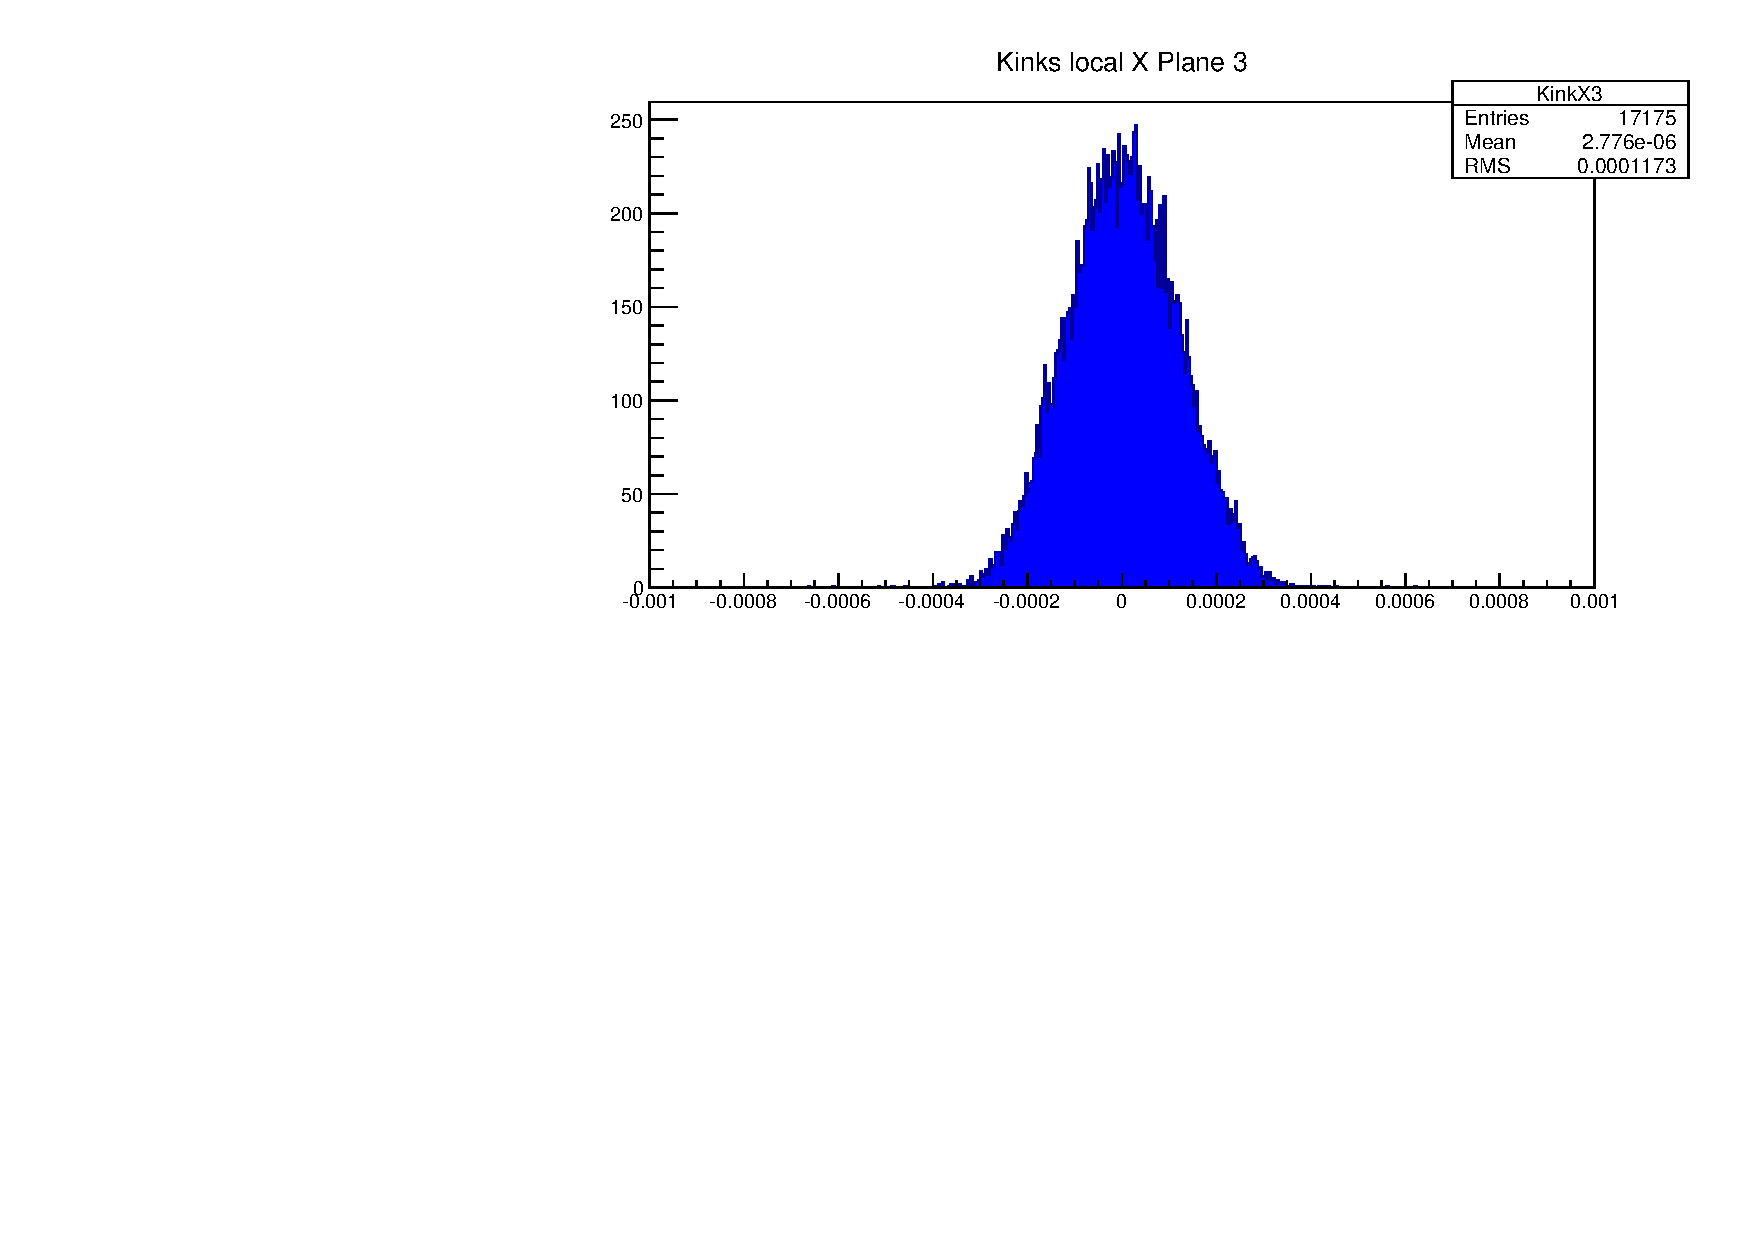
\includegraphics[scale=0.5]{figures/KinkX3Local-313-Wrong.pdf}}
%\subfloat{\label{fig:beamE5B1} 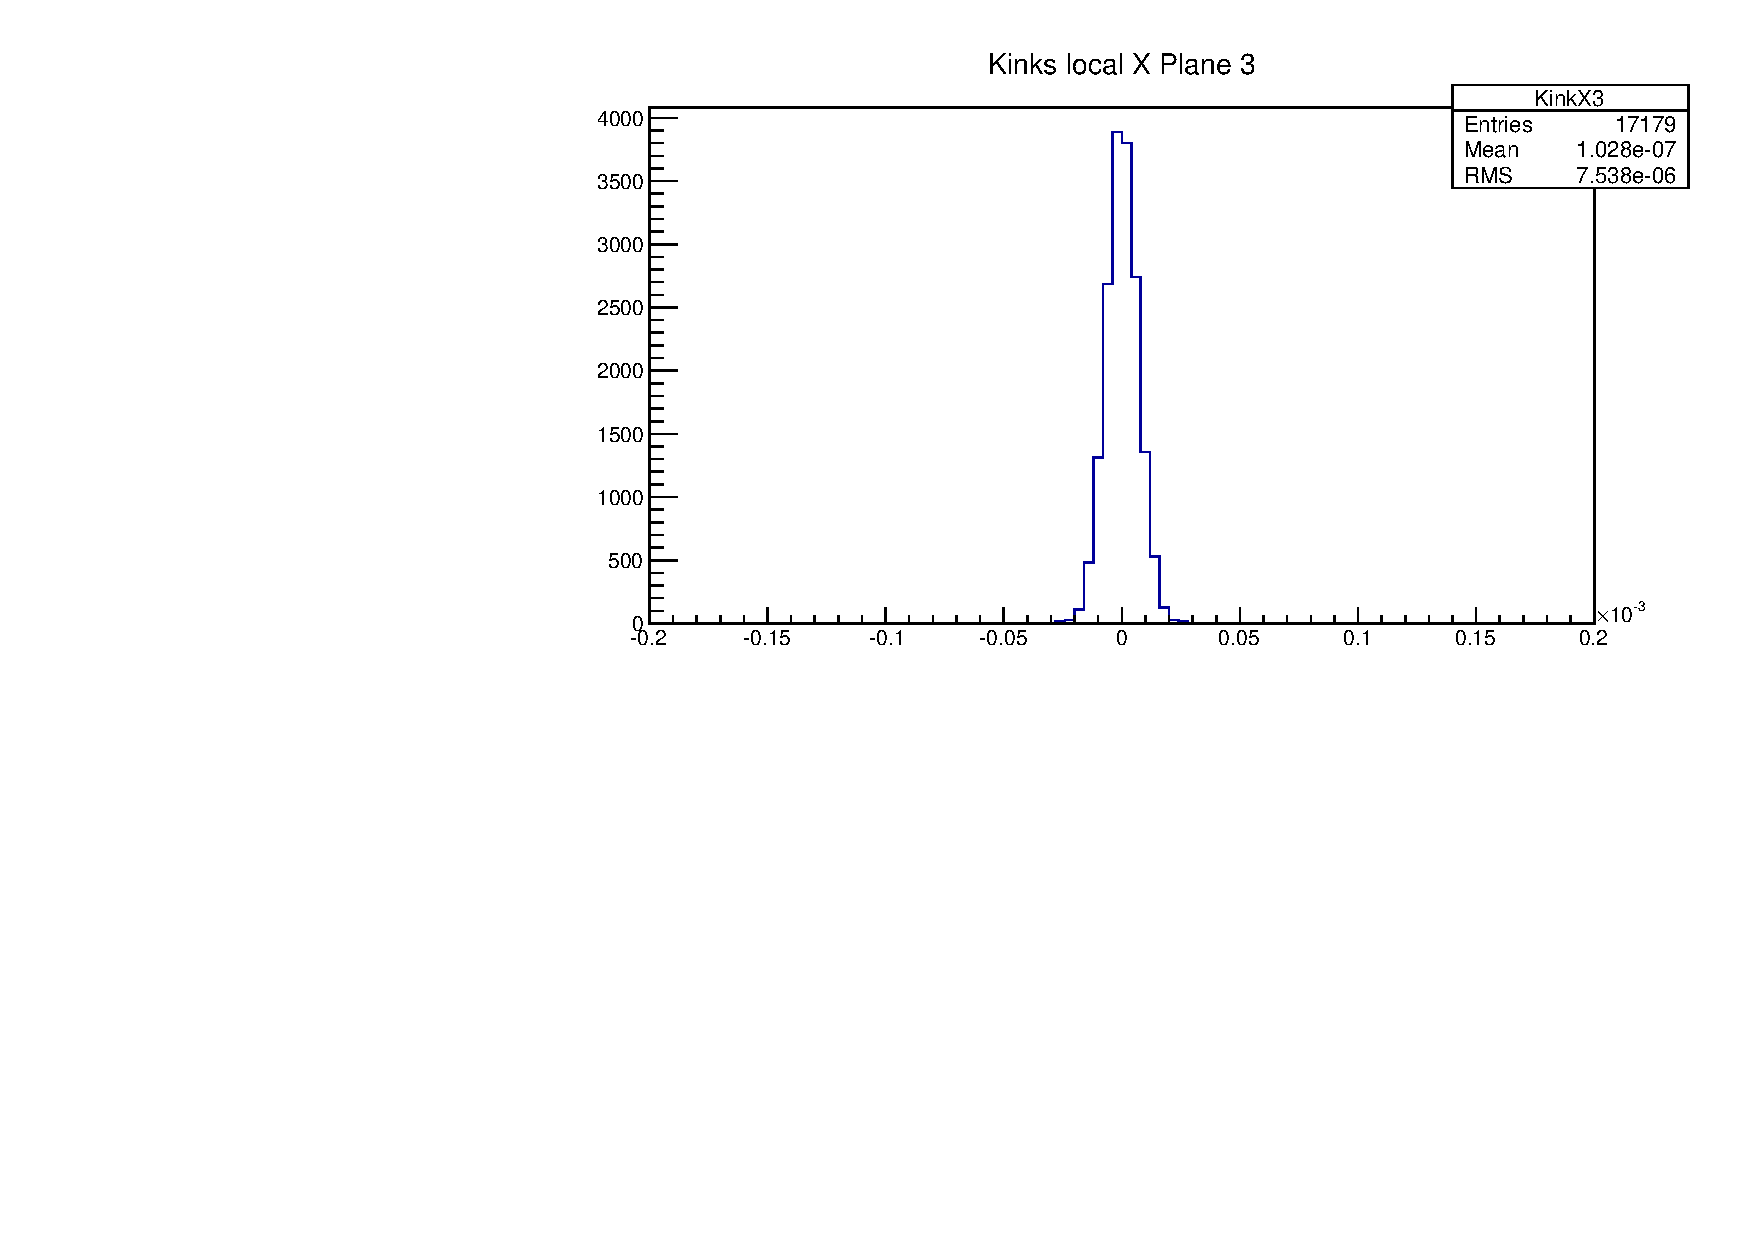
\includegraphics[scale=0.5]{figures/KinkX3Local-313-Corr.pdf}}
%\caption{The kink angles for both descriptions. The left has much larger kinks since this has not been incorporated into the scattering}
%\label{fig:kinkRad}
%\end{figure}
%
%\subsection{APIX mapping}
%
%\begin{figure}[H]
%\hspace{-35mm}
%\subfloat{\label{fig:beamE5B1} 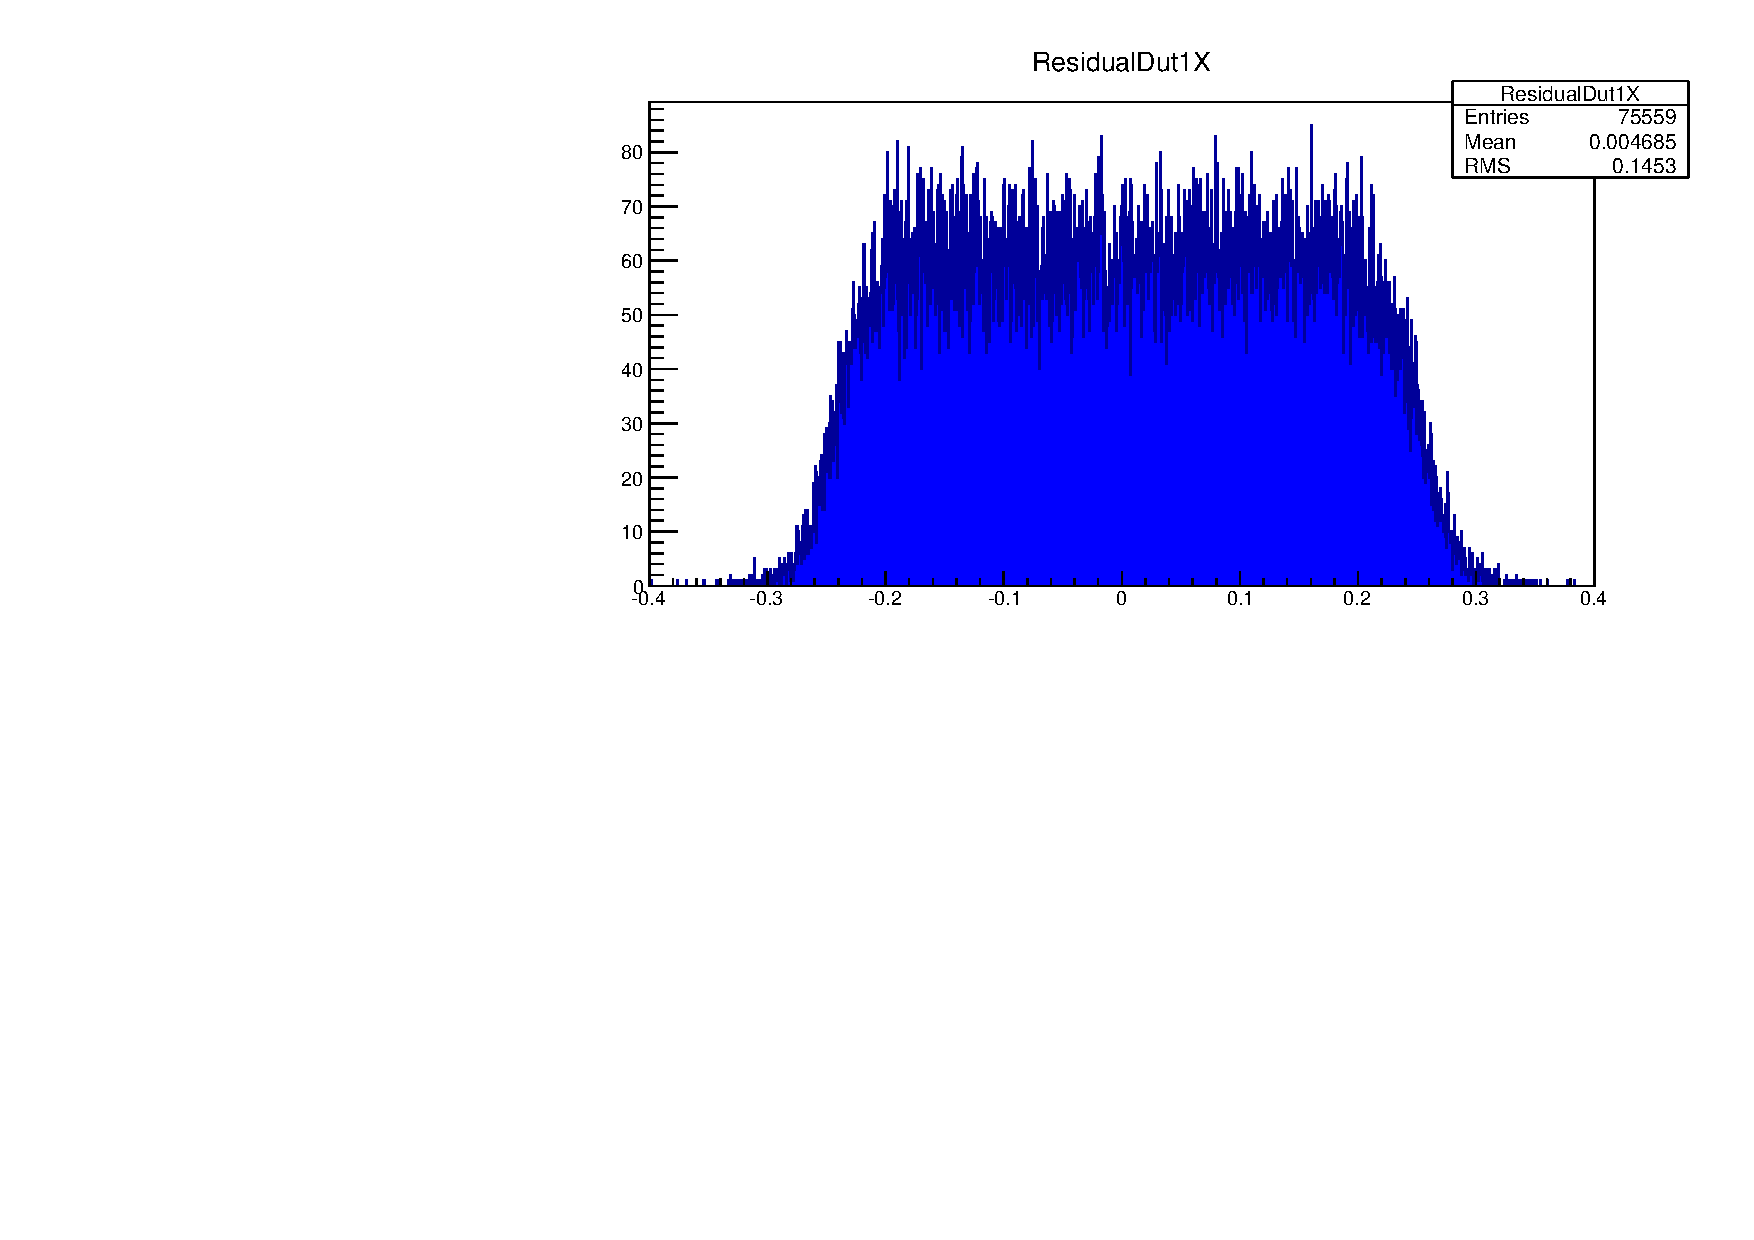
\includegraphics[scale=0.5]{figures/resX1D21.pdf}}
%\subfloat{\label{fig:beamE5B1} 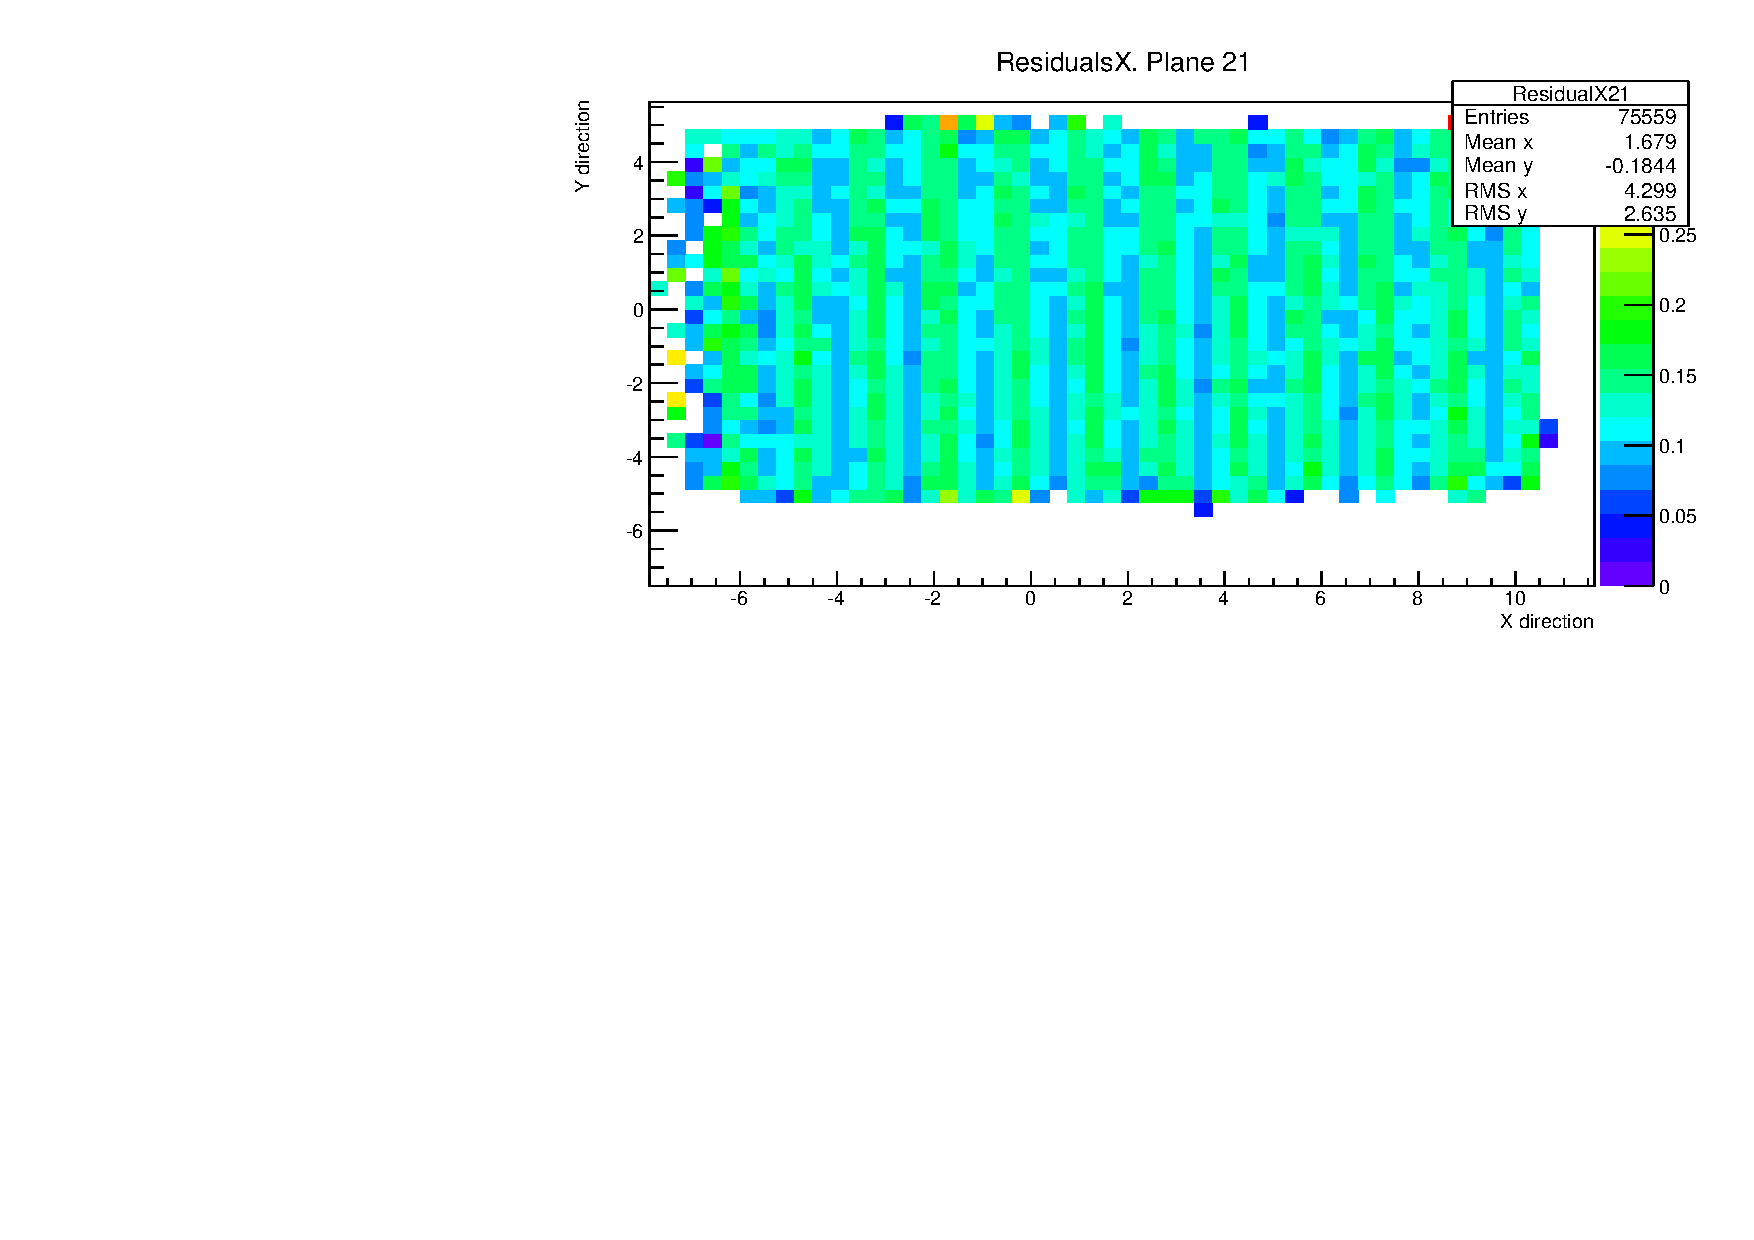
\includegraphics[scale=0.5]{figures/XRes2D21.pdf}}
%\caption{The residual from plane 21 inclusive and over the detector surface. DESY testbeam 4 GeV}
%\label{fig:kinkRad}
%\end{figure}
%
%
%\subsection{SCT strip}
%
%\subsection{Alibava strip}
%
%\subsection{Magnetic fields (no DUT)}
%
%\subsection{X0}
%
%\newpage
%
%\begin{figure}[H]
%\hspace{-35mm}
%\subfloat{\label{fig:beamE5B1} 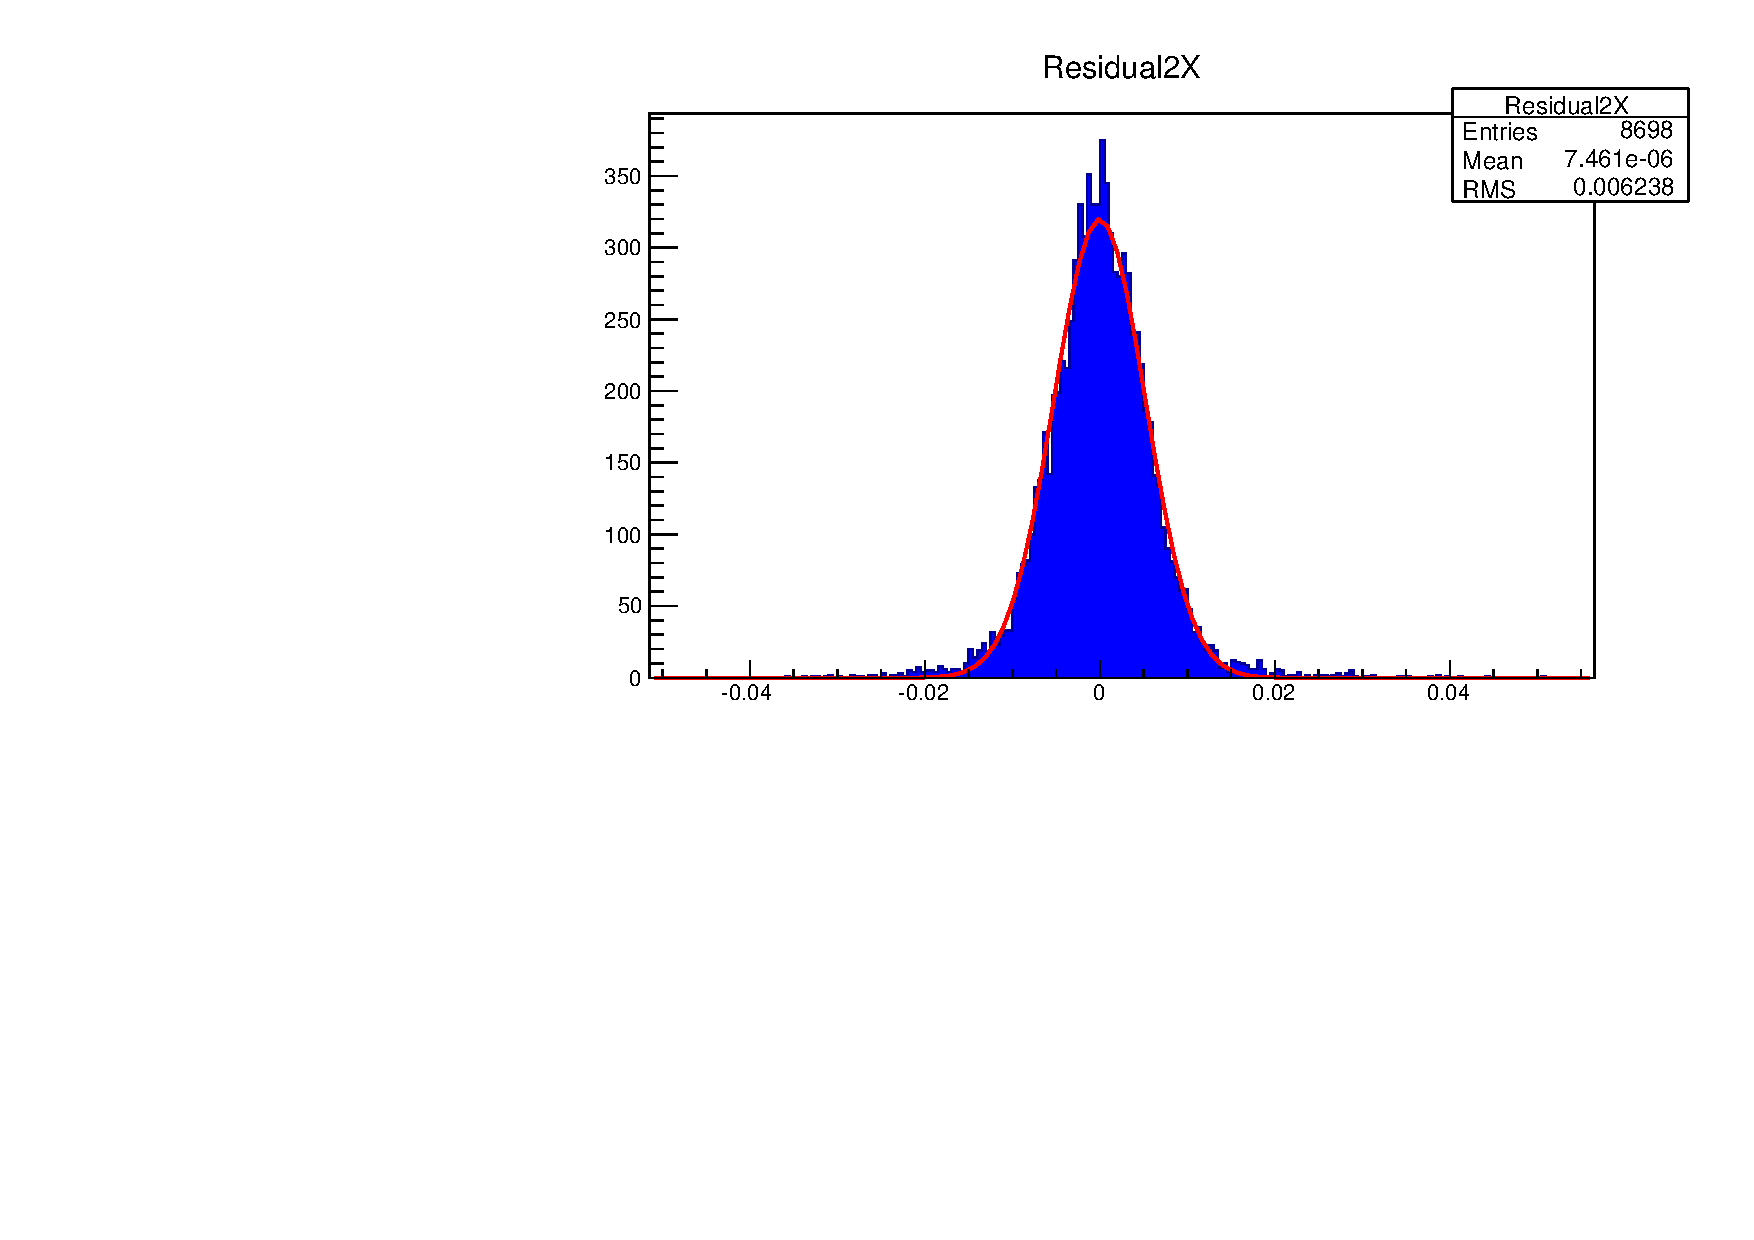
\includegraphics[scale=0.5]{figures/Sensor241-plane2ExcludeXRes.pdf}}
%\subfloat{\label{fig:beamE5B1} 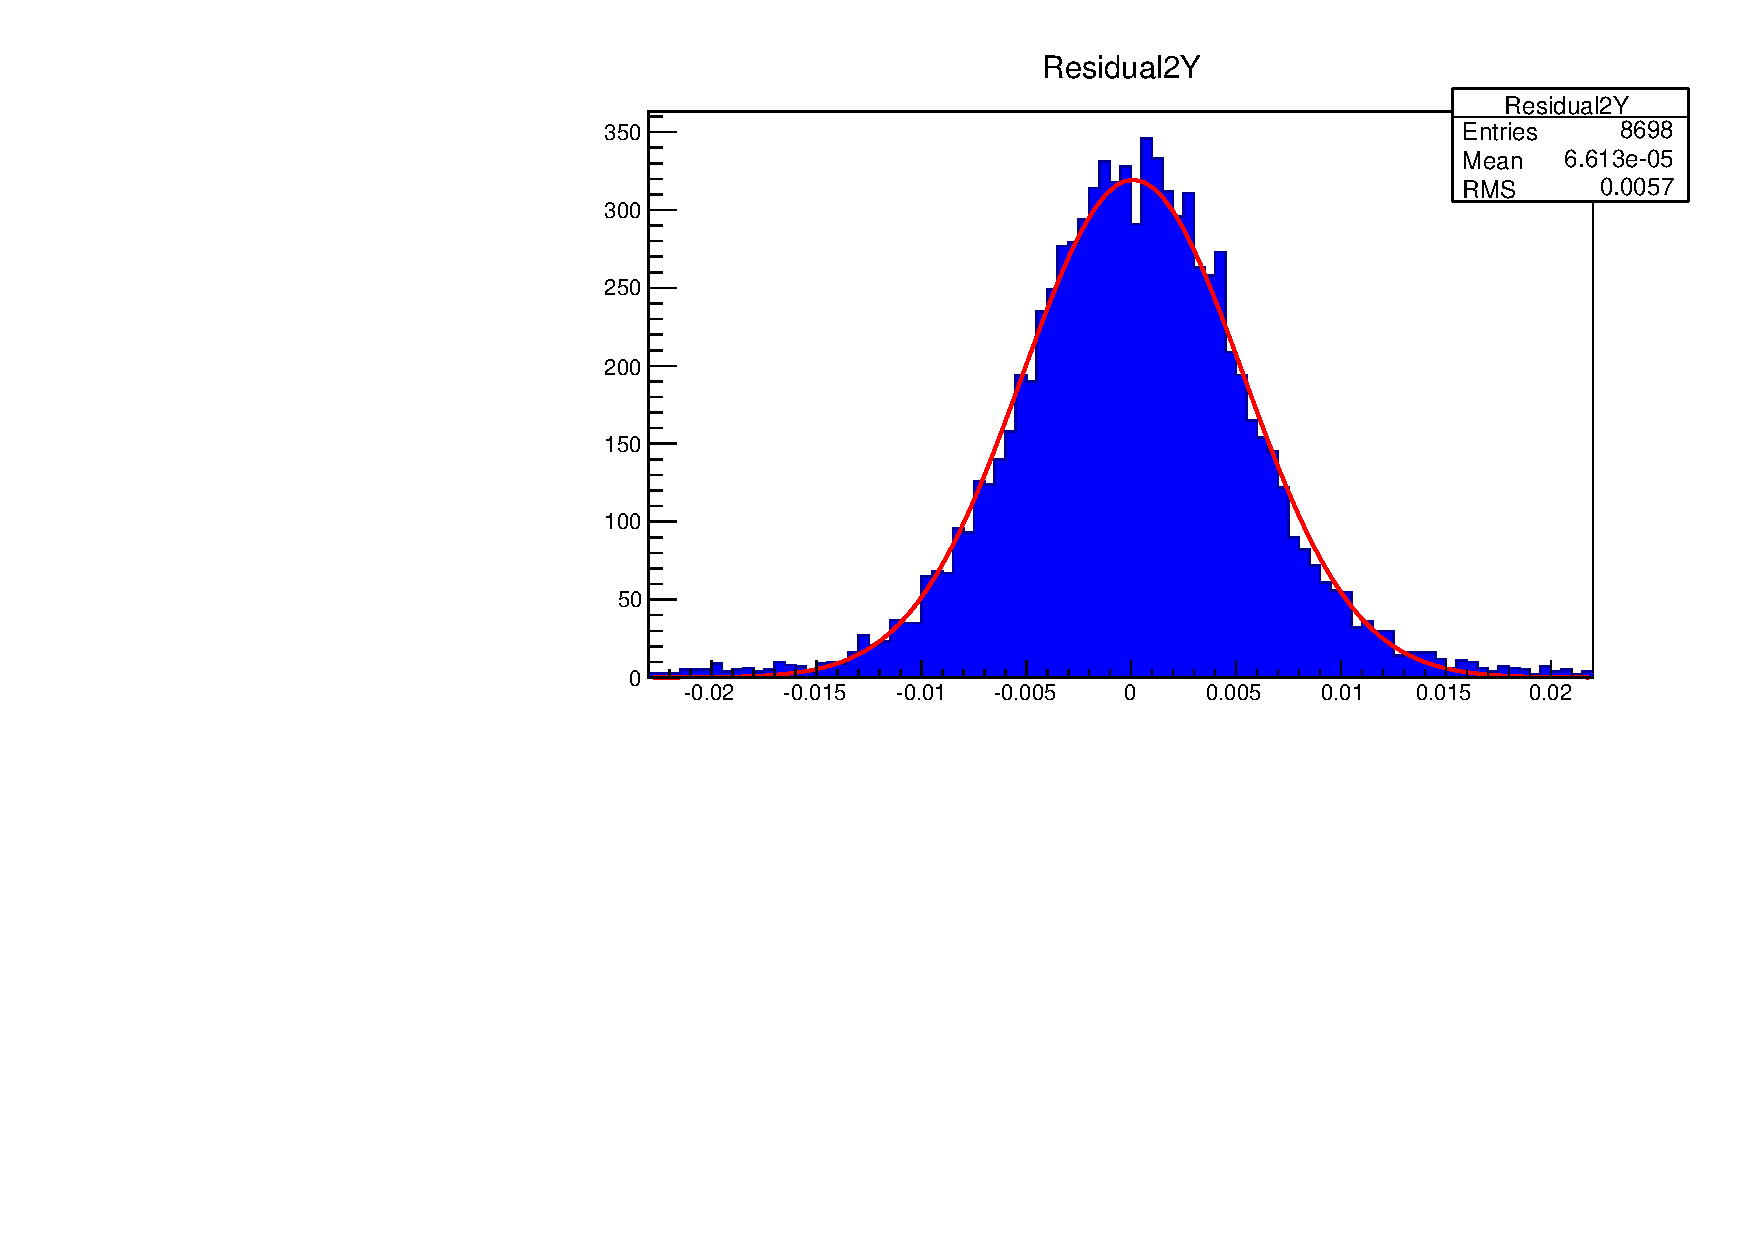
\includegraphics[scale=0.5]{figures/241-plane2ExcludeYRes.pdf}}
%\caption{}
%\label{fig:energy0}
%\end{figure}
%
%\begin{figure}[H]
%\hspace{-35mm}
%\subfloat{\label{fig:beamE5B1} 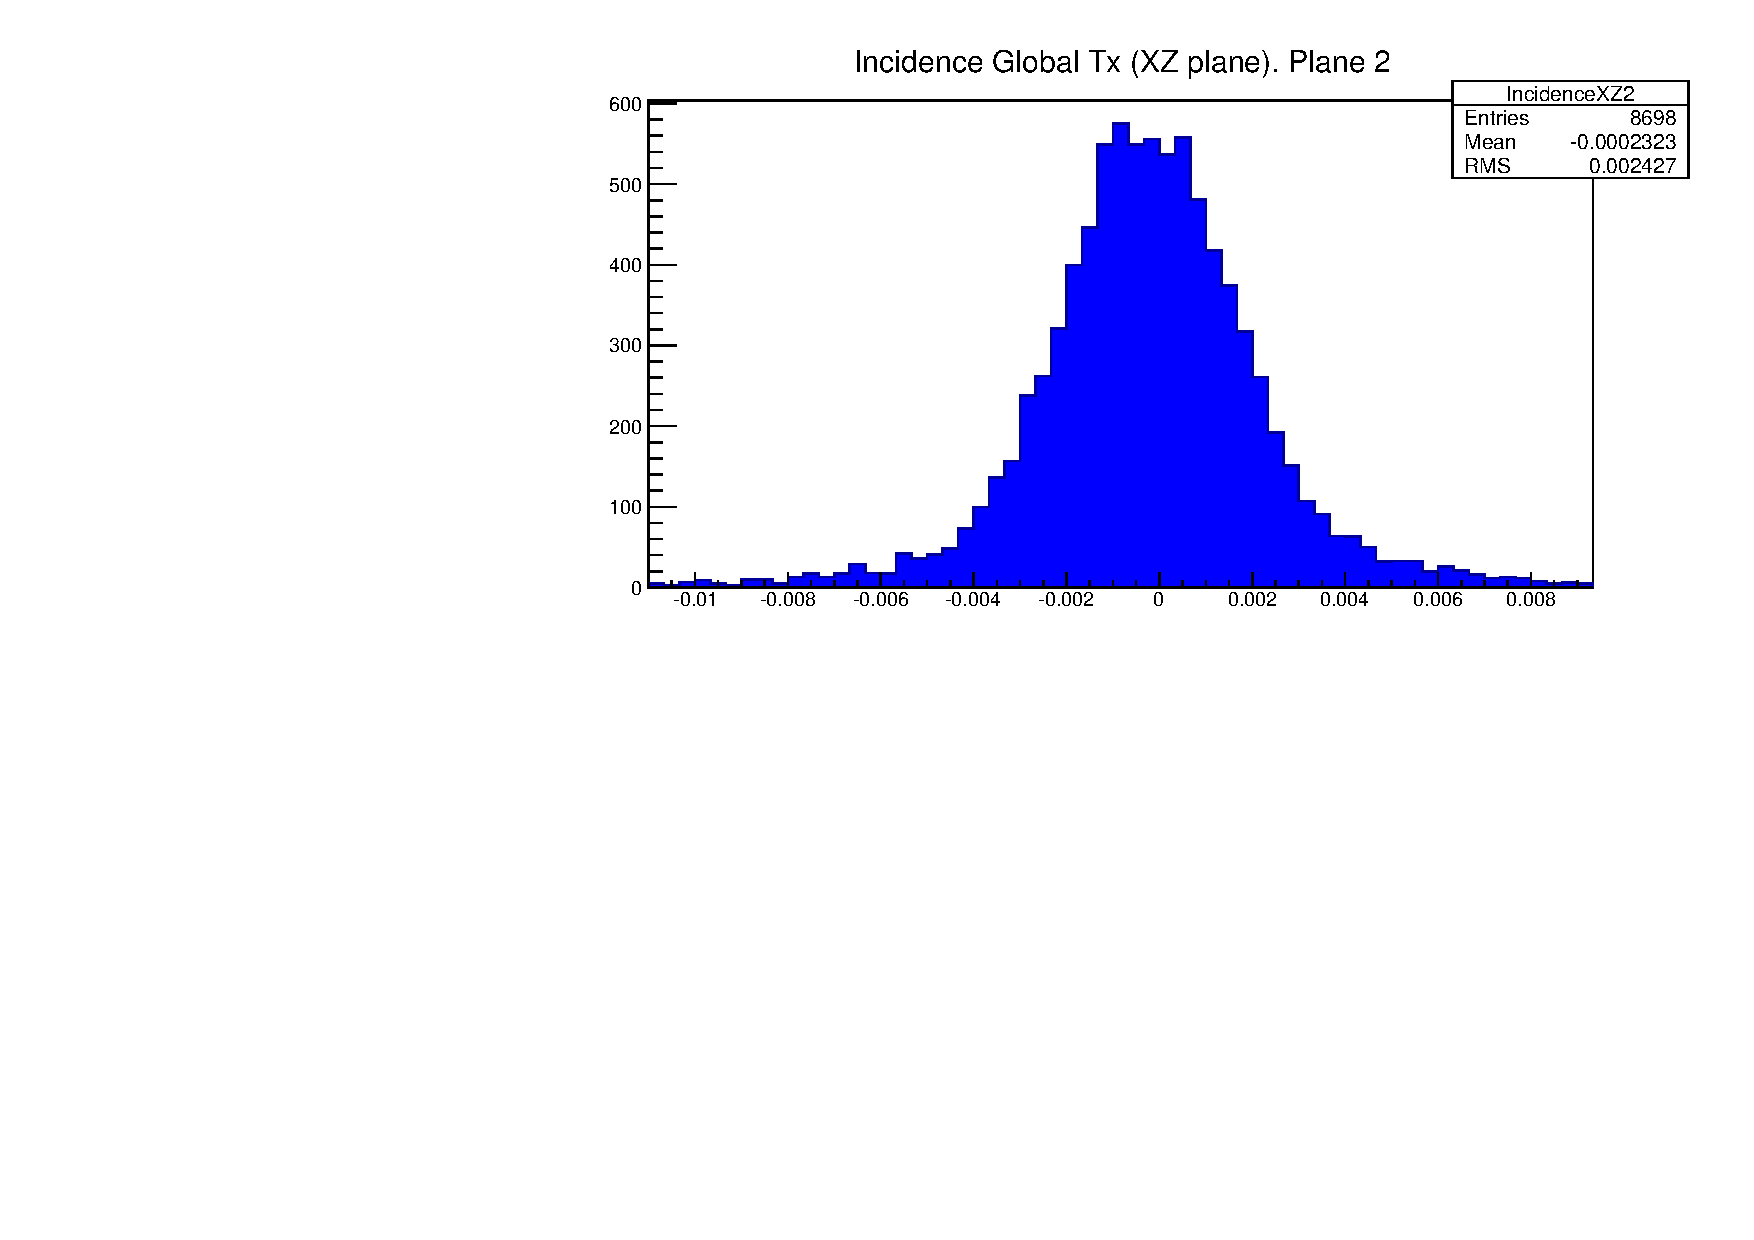
\includegraphics[scale=0.5]{figures/241-plane2ExcludeXInc.pdf}}
%\subfloat{\label{fig:beamE5B1} 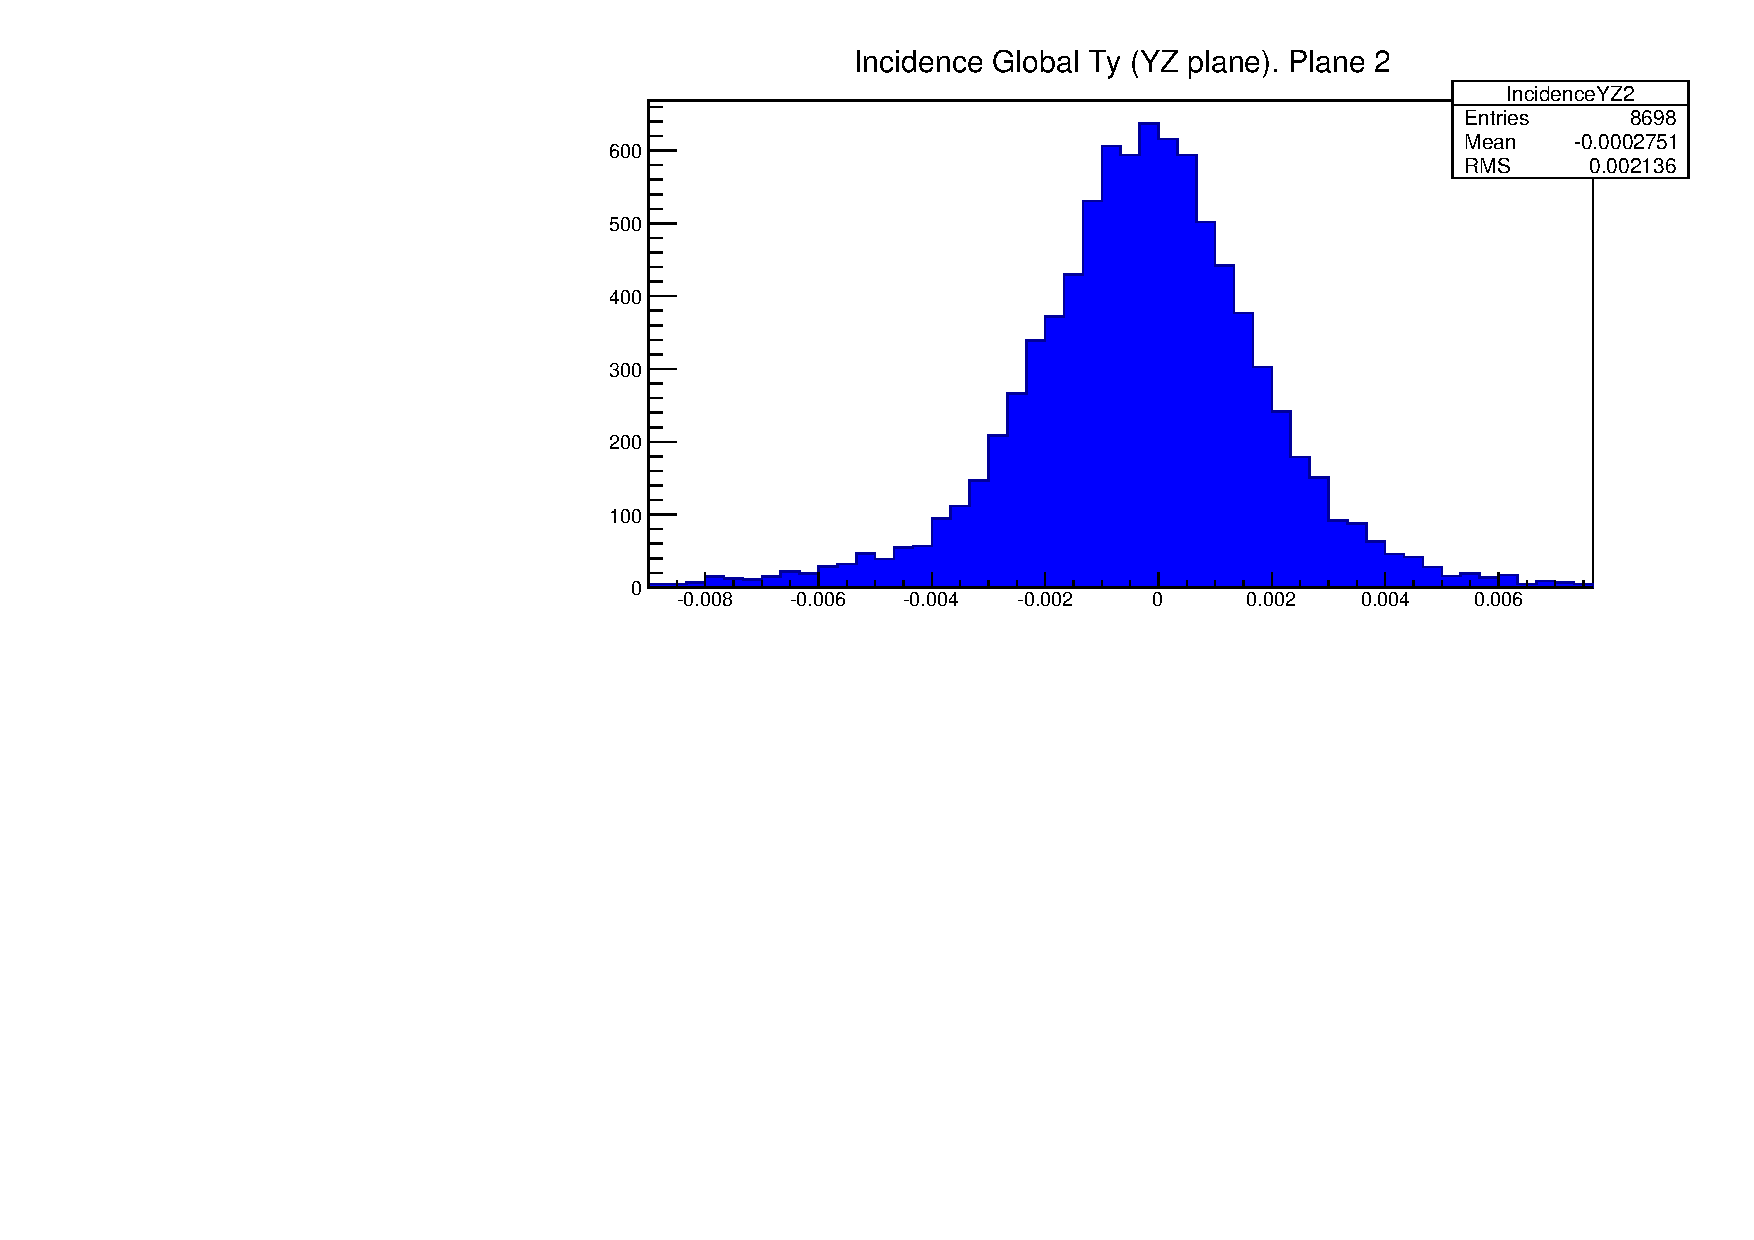
\includegraphics[scale=0.5]{figures/241-plane2ExcludeYInc.pdf}}
%\caption{}
%\label{fig:energy0}
%\end{figure}
%
%
%\begin{figure}[H]
%\hspace{-35mm}
%\subfloat{\label{fig:beamE5B1} 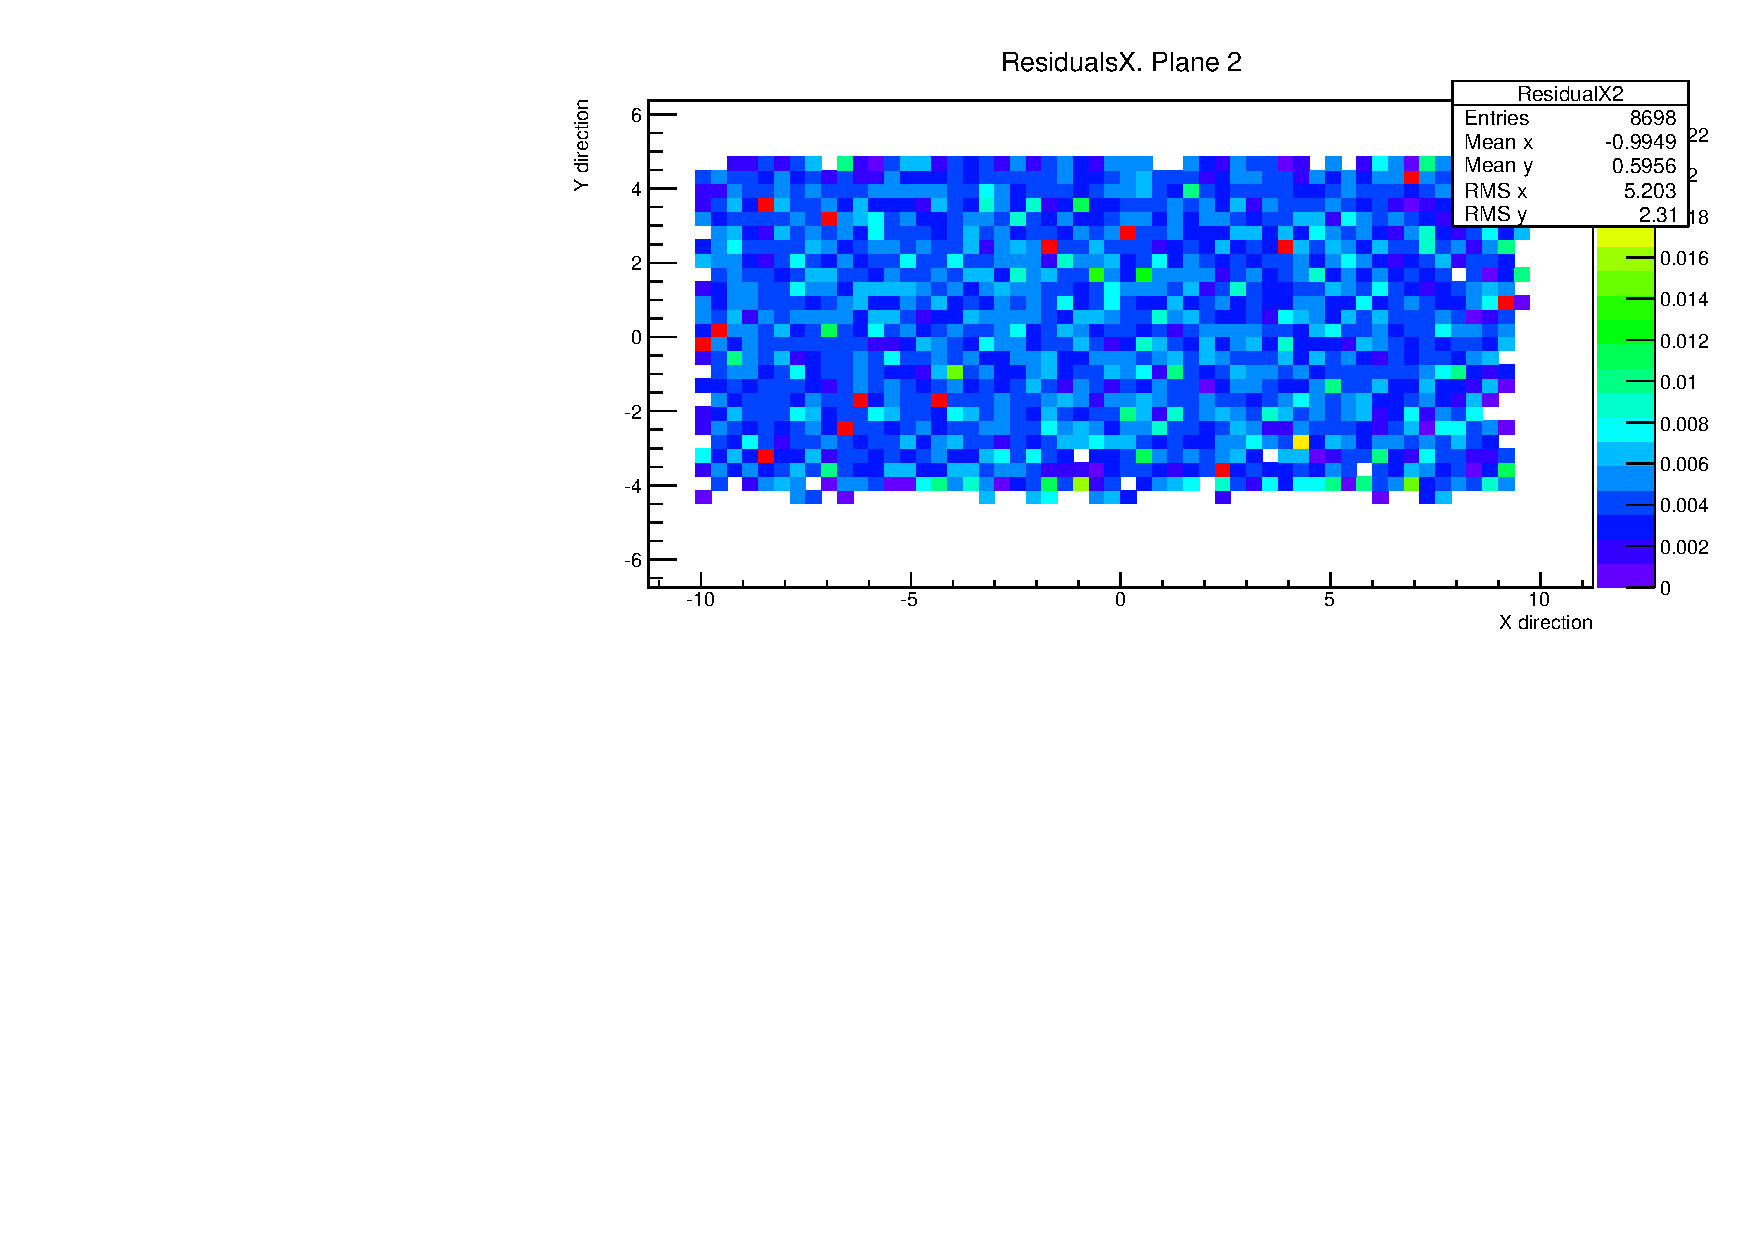
\includegraphics[scale=0.5]{figures/241-plane2ExcludeXRes2D.pdf}}
%\subfloat{\label{fig:beamE5B1} 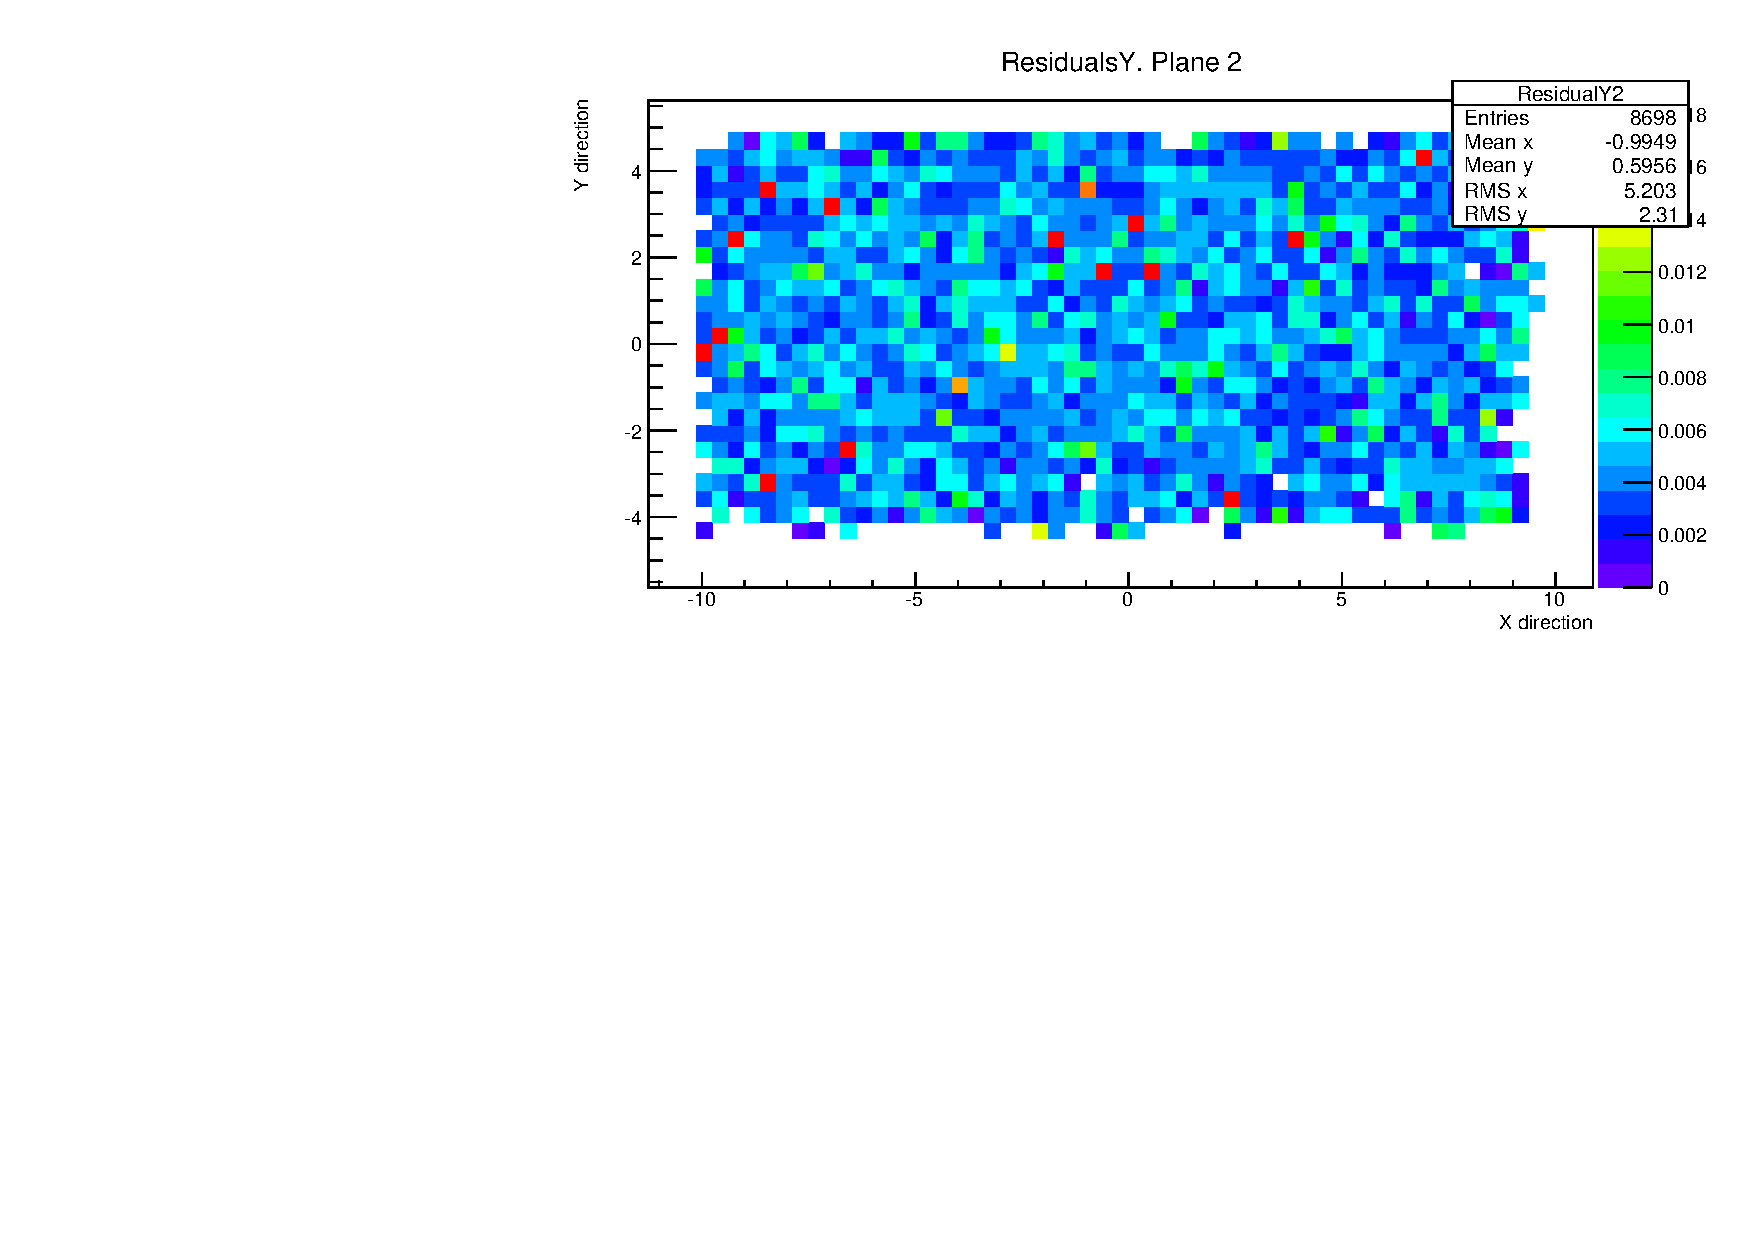
\includegraphics[scale=0.5]{figures/241-plane2ExcludeYRes2D.pdf}}
%\caption{}
%\label{fig:energy0}
%\end{figure}
%
%\begin{figure}[H]
%\hspace{-35mm}
%\subfloat{\label{fig:beamE5B1} 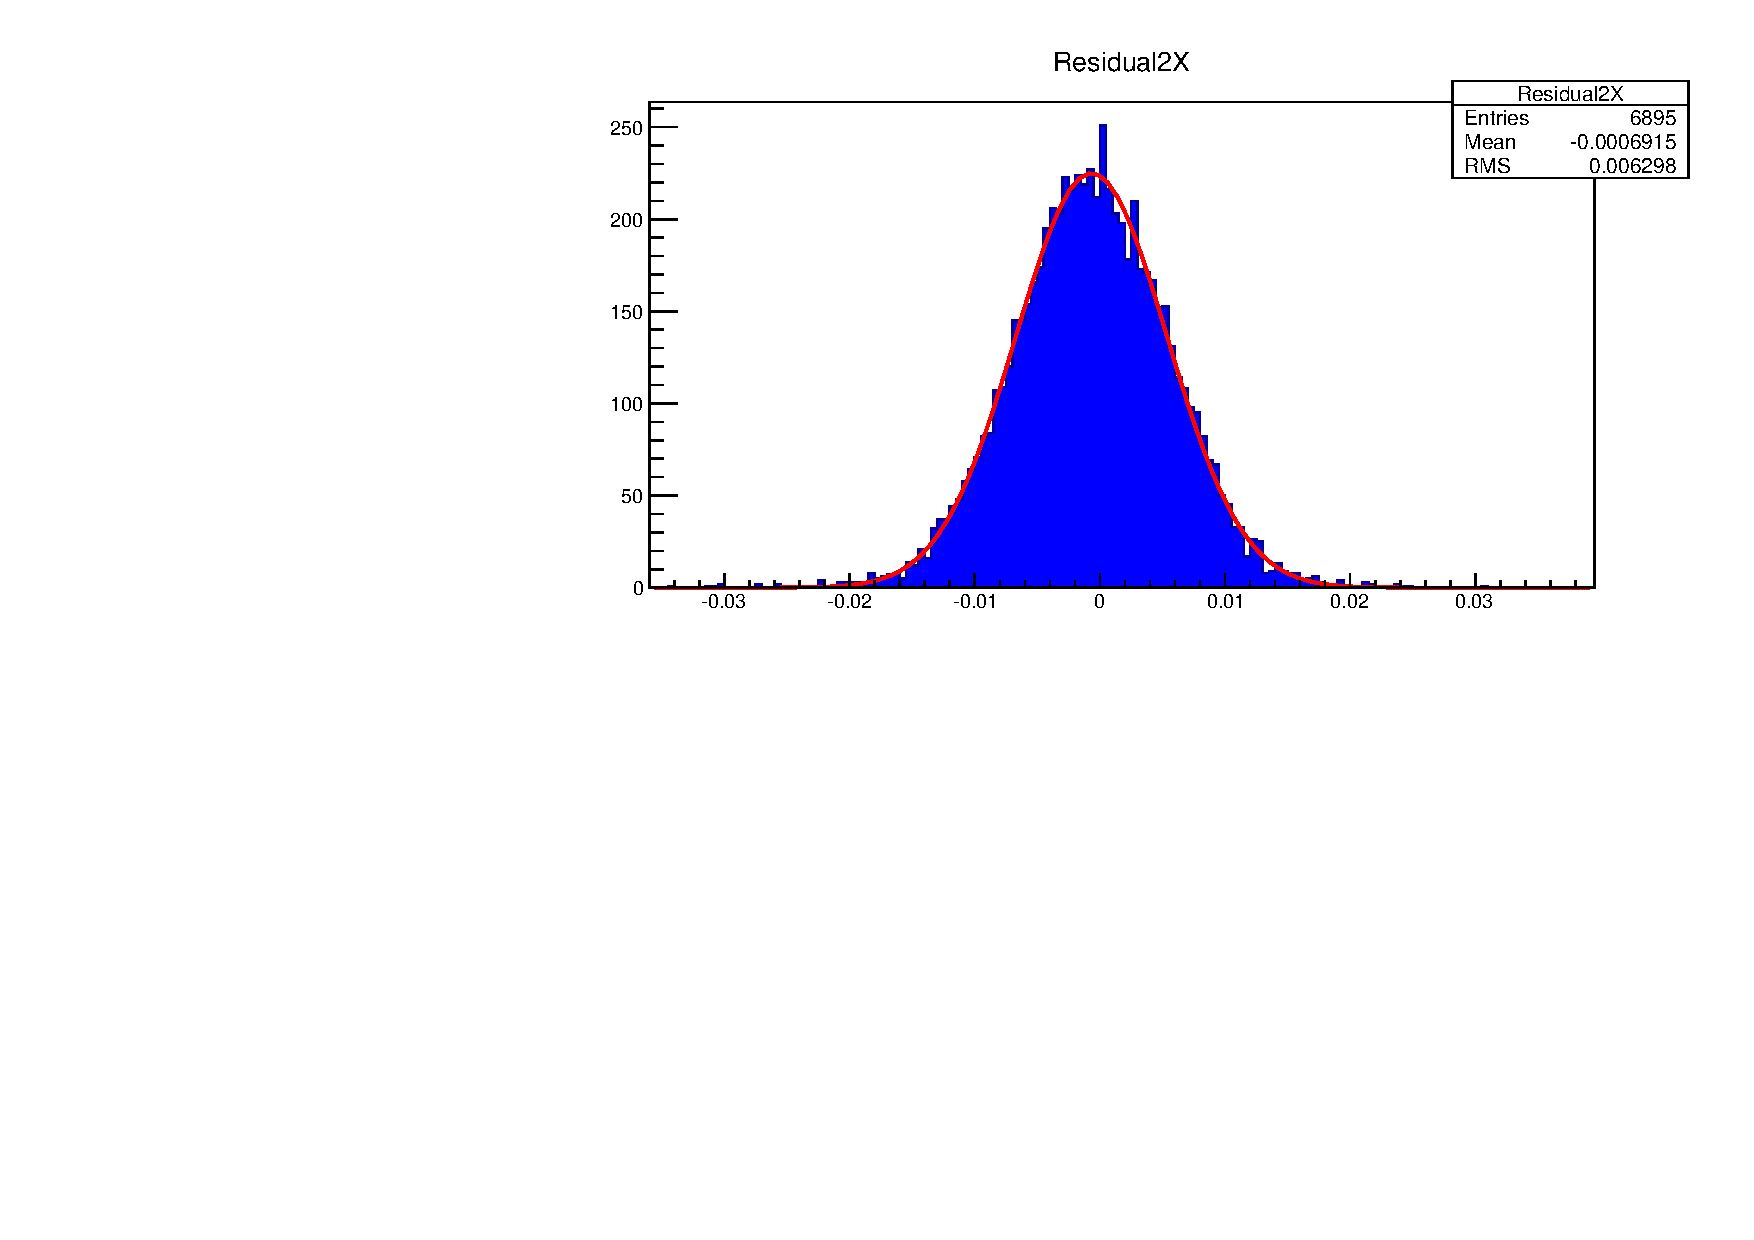
\includegraphics[scale=0.5]{figures/resX286-plane2Exc.pdf}}
%\subfloat{\label{fig:beamE5B1} 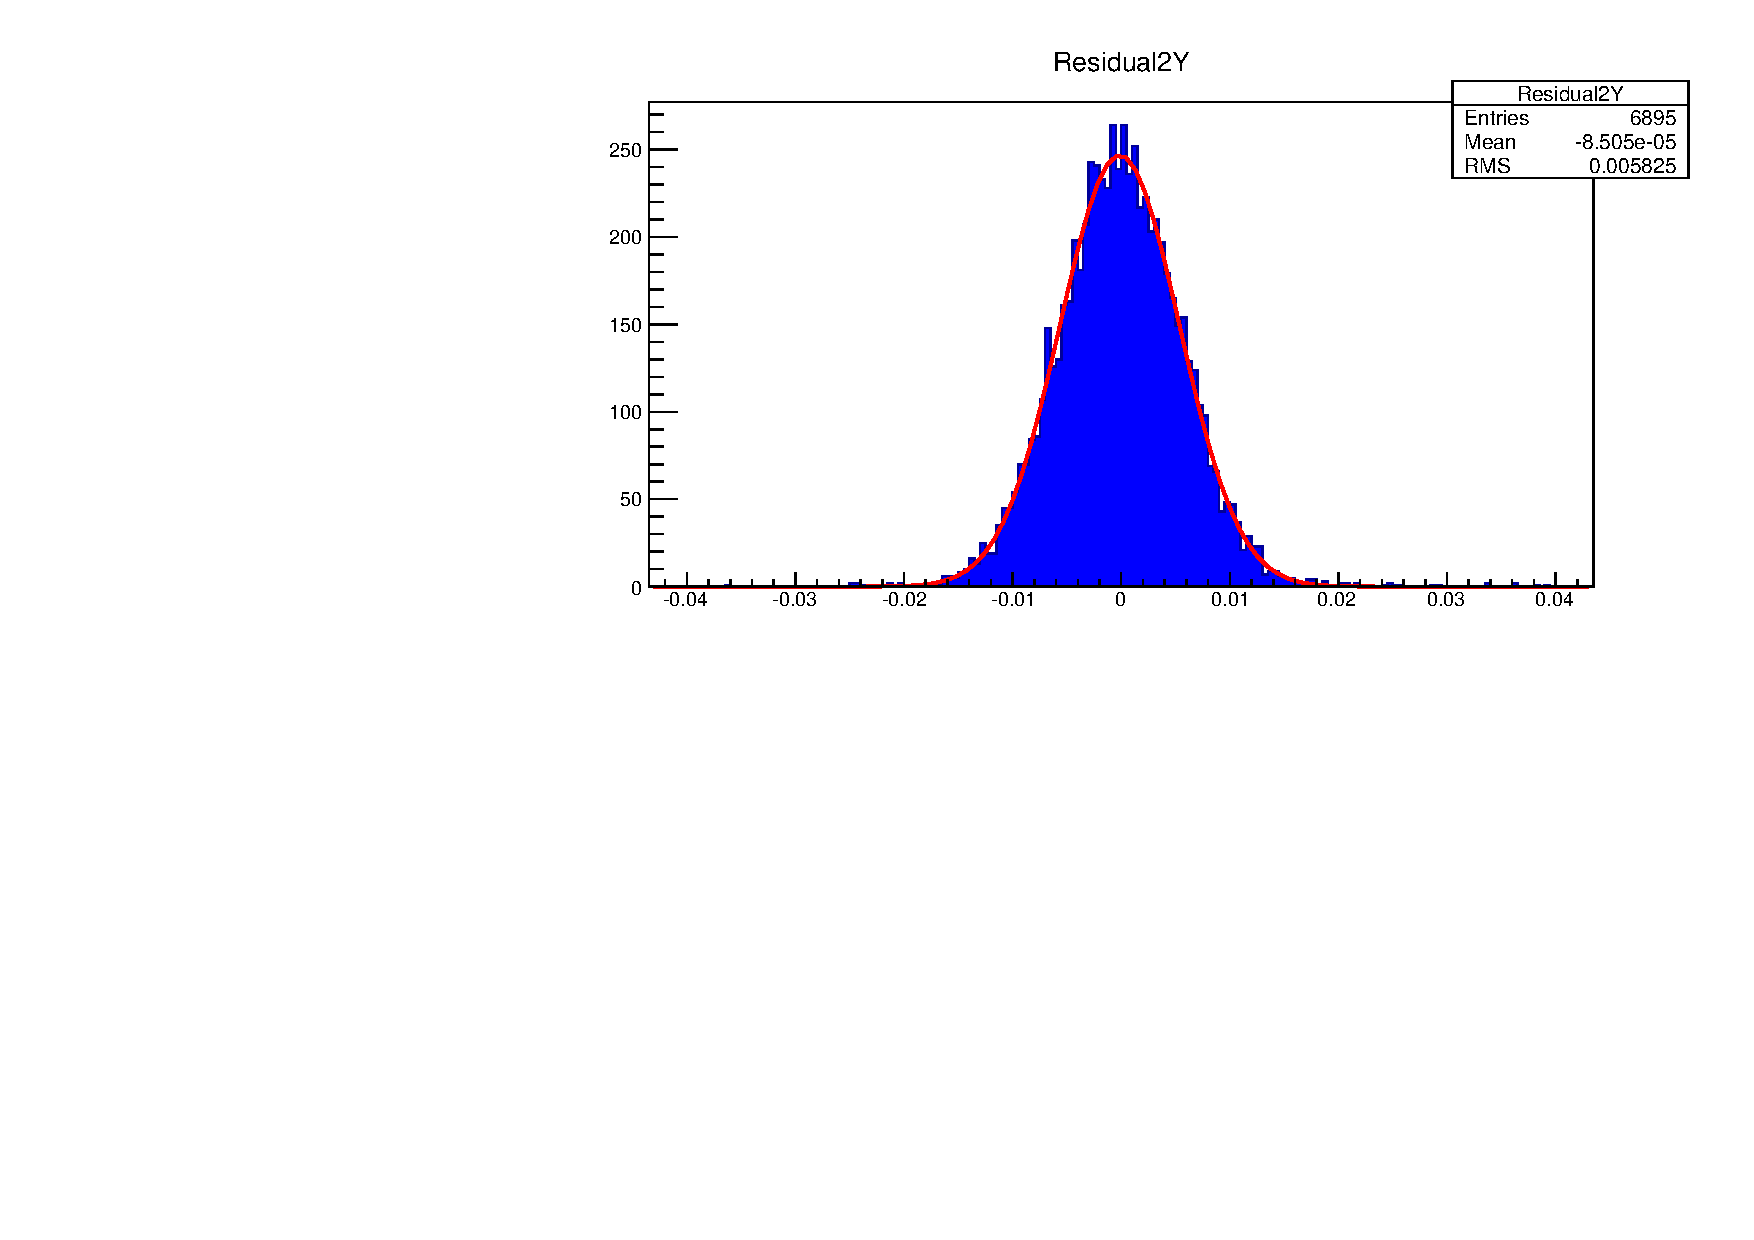
\includegraphics[scale=0.5]{figures/resY286-plane2Exc.pdf}}
%\caption{}
%\label{fig:energy0}
%\end{figure}
%
%\begin{figure}[H]
%\hspace{-35mm}
%\subfloat{\label{fig:beamE5B1} 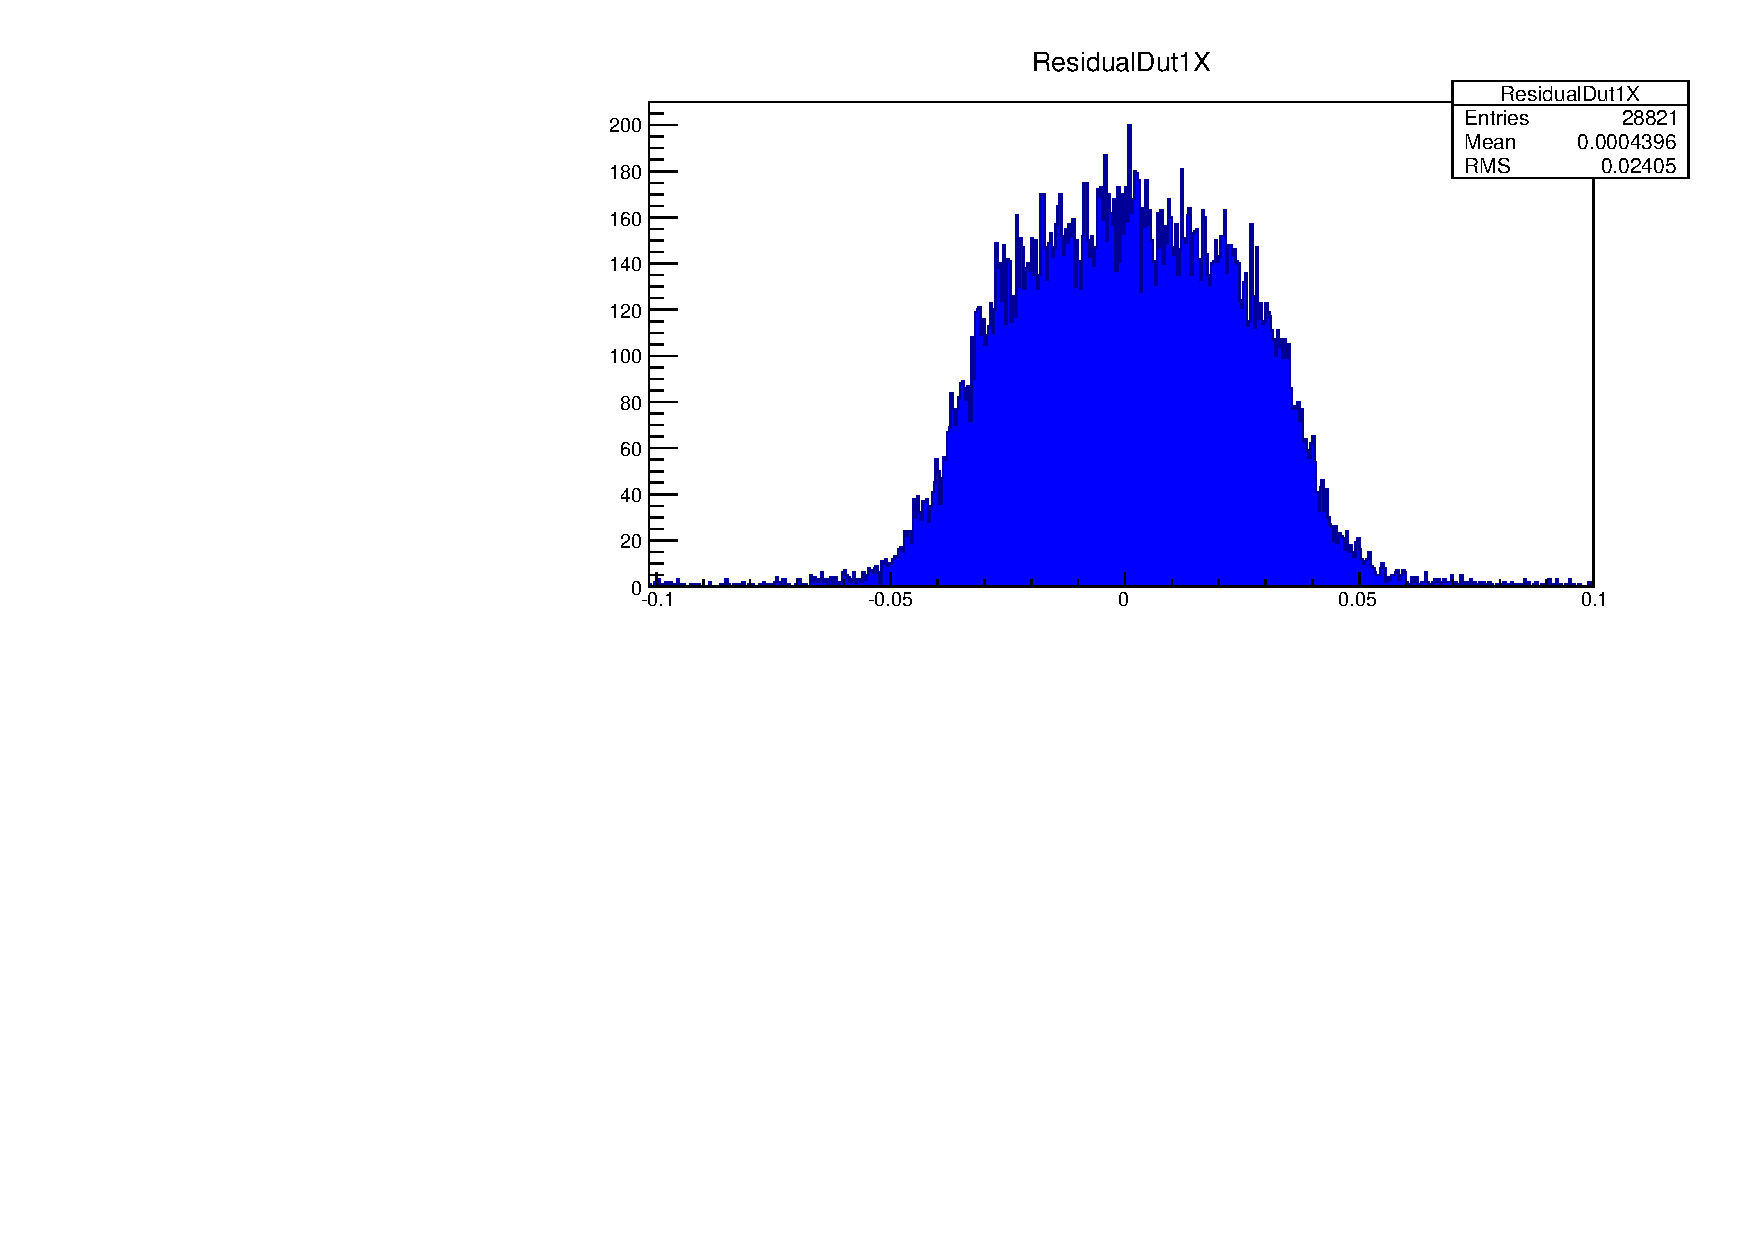
\includegraphics[scale=0.5]{figures/strip703Res.pdf}}
%\subfloat{\label{fig:beamE5B1} 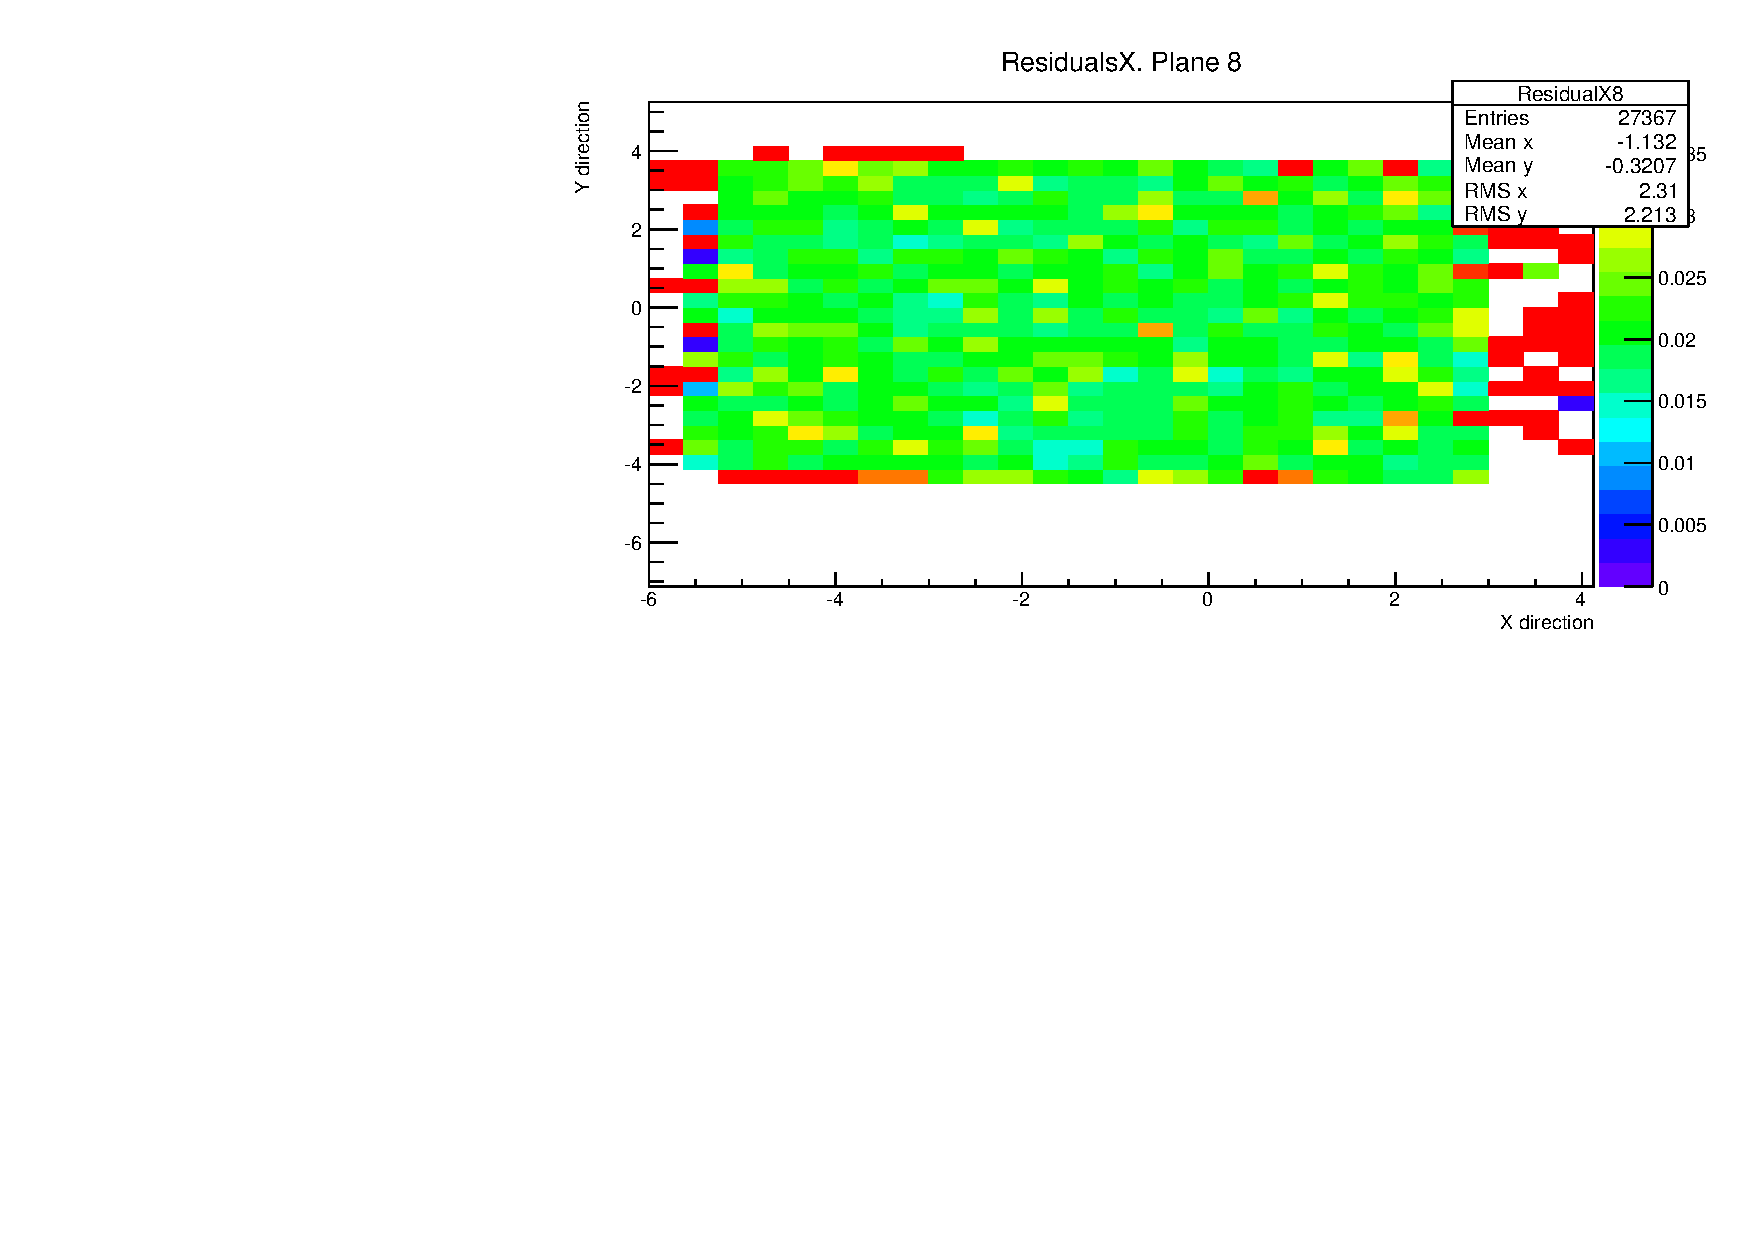
\includegraphics[scale=0.5]{figures/strip703Res2D.pdf}}
%\caption{}
%\label{fig:energy0}
%\end{figure}
%
%
%
%
%\subsection{Examples.}

%This can be seen as the relationship between moving a track a particular displacement and its intersection with a plane.


%The \emph{point correction matrix} $PC(X,Y,Z, \alpha,\beta,\gamma)$ is of the from.
%\[ \left( \begin{array}{cccccc}%
%1 & 0 & \frac{\partial d_0}{\partial d_2}   \\
%0 & 1 & \frac{\partial d_1}{\partial d_2}  \\
%\end{array} \right)\] 








\clearpage
\chapter{Examples}
\label{example}

Examples which are installed with EUTelescope can be run immediately. The only additional requirement is you have access to the DESY afs. A brief outline of some examples with be given below to show what can be done with the fitter. All examples in jobsub/examples/GBL directory in EUTelescope. A step by step guide of what parameters to change in the config is given in the README for each example. The name is black is the name given in the examples directory.

\begin{description} 
\item[noDUTExample] This example demostrates the use of the fitter with magnetic fields and varying beam energies.
\item[Quad] Quad module with reference DUT at the DESY testbeam 
\item[QuadSLAC]  Quad module and reference DUT at the SLAC testbeam.
\item[Pixels] High radiation length enviroment using the gear file to describe dead material. Two APIX devices at DESY testbeam.
\item[mappingAPIX] Two APIX DUTs using the mapping processor between channel number and geometric cluster position.
\item[mappingAPIXSLAC] This is the same as the other mapping example but at SLAC and with highly irradiated sensors. The highly irradiated sensors make the reconstruction much harder.
\item[SCT] Strip example which has been used for detailed efficiency measurements. This example contains the ROOT output formats which include TBMon.
\item[StripAlibava] ATLAS12 strip device using the alibava system as readout. High radiation length downstream causes larger beam divergences than expected at DESY beam.
\item[X0] The use of the kink angle estimation is demostrated here. The results of this example should be investigated more fully. However the track fitting and alignment is completed. 
\end{description} 
\clearpage


\end{document}

